\chapter{Computer Science}
\label{chapter:computer-science}

\section{Solution Design}
\label{chapter:design}

This chapter aims to fully describe the solution design from a top to bottom approach. First of all, the general idea of the design is described, abstracting every detail to easily understand the whole. Later on, the different sections of the design are explained with all their characteristics described. The implementation details are left for the following chapters, whereas here we only focus on the ideas and methods used.

In short, the solution to the problem of studying what an observer near a black hole would see is a ray tracer, that is, a device that computes the origin of the rays of light that arrives to a virtual camera placed in a virtual universe.

This work implements a general relativity ray tracer; \ie, a ray tracer for which the path followed by light is not always a straight line.

In \autoref{sec:gendesc}, the layout of the solution is depicted, whereas in \autoref{sec:parallel}, the parallelization designed is explained. \autoref{sec:pinhole} explains the pinhole camera model, describing the identification of each pixel on the camera with a lightlike particle coming from the celestial sphere. Finally, \autoref{sec:initcond} and \autoref{sec:numerical} describes the necessary work to numerically solve the geodesic equations.

\subsection{General Description}
\label{sec:gendesc}

Imagine a spacetime defined by a Kerr metric, with a black hole on its centre, and a camera with a digital sensor placed near it.

As we have studied, all rays that hit the sensor have followed a geodesic to finally arrive to the camera, and their paths are of great interest for us: the origin of the ray will tell us what the particular pixels see and the curvature of the geodesic will let us understand the geometric nature of the spacetime.

For every pixel on the sensor, the ray tracer work can be abstracted as a function that computes the path of the ray that hit it. Therefore, from the pixel coordinates, $p = (p_x, p_y)$, it computes the geodesic path followed by the ray.

This point is computed using the \ac{ODE} system described in \autoref{theo:eqsmotion}, derived from the Kerr spacetime. Therefore, a numerical solver for such systems is needed, along with the initial conditions of each ray. This conforms an \ac{IVP}, a kind of well-known problem whose numerical solutions are widely studied.

Abstracting all these tasks out, the general outline of the ray tracer is described on \autoref{alg:raytracer}.

\begin{algorithm}
	\caption{High-level abstraction of the ray tracer}
	\label{alg:raytracer}
	\begin{algorithmic}[1]
		\Function{Ray Tracer}{}
		\State ODEsystem $\gets$ Geodesics equations for the Kerr spacetime
		\State Camera $\gets$ Pinhole camera model
		\State Geodesics $\gets \{\emptyset\}$
		\For{pixel $p = (p_x, p_y)$ in the Camera sensor}
		\State initCond $\gets$ initConditions($p_x$, $p_y$)
		\State $\gamma_{xy} \gets$ solveInitValueProblem(ODEsystem, initCond)
		\State Geodesics $\gets$ Geodesics $\cup$ $\gamma_{xy}$
		\EndFor
		\Return{Geodesics}
		\EndFunction
	\end{algorithmic}
\end{algorithm}

The solution designed for the ray tracer is based on the algorithm described in \cite{thorne15}, which assumes the following:
\begin{enumerate}
	\item The spacetime is defined by the Kerr metric written in \ac{BL} coordinates (see \autoref{eq:kerrmetric}), with a black hole in the centre of the spatial coordinates parametrized by its spin $a$. Its mass is assumed to be 1.
	\item The \ac{FIDO} is a locally non-rotating observer. We define a family of \acp{FIDO} at rest in space with orthonormal basis vectors $\{e_r, e_\vartheta, e_\varphi\}$, pointing along the spatial coordinate lines.
	\item A camera is placed outside of the horizon of the black hole.
	\begin{enumerate}
		\item The position of the camera is described by the coordinates $\{r_c, \vartheta_c, \varphi_c\}$.
		\item The camera speed with respect to the \ac{FIDO} is noted as $\beta$.
		\item The direction of motion relative to the \ac{FIDO} is described by a unit vector $B$ in the camera's reference frame.
		\item We set up a right-handed coordinate system placed on the camera's reference frame, with the orthonormal basis $\{e_x, e_y, e_z\}$, where
		\begin{itemize}
			\item $e_y$ is identified with $B$; \ie, it points to the direction of motion of the camera.
			\item $e_x$ is perpendicular to $e_y$ and contained on the plane $\langle e_{\widehat{r}}, e_{\widehat{\vartheta}} \rangle$.
			\item $e_z$ is perpendicular to $e_x$ and to $e_y$.
		\end{itemize}
		\item We set up a spherical coordinate system derived from the previous one, noted as $\{\vartheta_{cs}, \varphi_{cs}\}$, where:
		\begin{itemize}
			\item $\vartheta$ is the polar angle with respect to the coordinate system origin.
			\item $\varphi$ is the azimuthal angle with respect to the coordinate system origin. The black hole is assumed to rotate in the positive $\varphi$ direction.
		\end{itemize}
	\end{enumerate}
\end{enumerate}

The algorithm consider a set of timelike geodesics arriving at the camera. These geodesics are then integrated backwards to obtain the ray's point of origin on the celestial sphere (at $r = \infty$). These points are noted as $(\vartheta', \varphi')$.

In short, the algorithm goal is to compute the following map
\begin{equation}
\label{eq:initmap}
(\vartheta_{cs}, \varphi_{cs}) \xmapsto{\mathfrak{h}_1} (\vartheta', \varphi')
\end{equation}
for each considered geodesic arriving at the camera.

\section{Parallelization Techniques}
\label{sec:parallel}

A ray tracer is in general highly parallelizable, and our design is not different: it performs the exact same operation on a large set of different data, namely it solves the \ac{ODE} system, whose equations (\autoref{theo:eqsmotion}) are always the same, on a large number of different initial conditions.

The idea behind the parallelization design is easy: for each parallelized node, we have to feed the numerical solver with a different initial condition, computed from each pixel of the image. Using the classic Flynn's taxonomy \cite{flynn72} terminology, our architecture follows a \ac{SIMD} paradigm, where a single generalized task works on multiple data streams in order to compute multiple results.

Ideally, we would like to design a completely parallel solution, in which we have the same number of nodes in the parallel architecture as pixels we have in the image. Although this is highly difficult for large images with the classic parallelization on \acp{CPU}, the new \ac{GPU} techniques will help us get closer to this goal.

\subsubsection*{General-Purpose Computing on Graphics Processing Units}

Historically, \acp{GPU} have been used to process tasks and data always related to computer graphic purposes, whereas \acp{CPU} have been used in general computation.

In recent years, a new powerful technique has been deeply studied: the so-called \ac{GPGPU}. Its goal is to use the \acp{GPU}, designed to have thousands of cores that can process data in parallel, to general purpose computing, not only computer graphics tasks.

Although each of the cores on a \ac{GPU} is much less powerful than a single \ac{CPU}, the great order of parallelization ---thousands of cores in a \ac{GPU} against just a few dozens of them on \acp{CPU}--- and the specific design to handle a parallel architecture makes the use of \ac{GPGPU} appealing when one wants to design an efficient solution.

Our ray tracer uses this paradigm, virtually parallelizing the computation of each geodesic in a different \ac{GPU} core. We say \emph{virtually} because the number of cores in a \ac{GPU} is always finite, and for large images, some computations will have to be serialized. However, as we will see in the following chapter, this will be transparent to us, developers, by using a proper \ac{GPGPU} library.

\subsubsection*{Parallelized Solution}

With this paradigm in mind, we can describe the parallelized solution by modifying the main loop on \autoref{alg:raytracer}, whose iterations will be split across all the nodes on the \ac{GPU}.

If we abstract the computation of the geodesic that hits one single pixel in a function, as shown in \autoref{alg:onepixel}, we can finally define the layout of the parallelized solution.

\begin{algorithm}[bth]
	\caption{Single pixel geodesic computation}
	\label{alg:onepixel}
	\begin{algorithmic}[1]
		\Function{ComputeGeodesic}{$p_x, p_y$, Geodesics}
		\State initCond $\gets$ initConditions($p_x$, $p_y$)
		\State $\gamma_{xy} \gets$ solveInitValueProblem(ODEsystem, initCond)
		\State Geodesics $\gets$ Geodesics $\cup \gamma_{xy}$
		\EndFunction
	\end{algorithmic}
\end{algorithm}

\autoref{alg:raytracer2} shows the parallelized solution following the \ac{SIMD} paradigm. The solution is similar to the one shown at \autoref{alg:raytracer} but with a little change: the loop is now parallelized and each pixel is computed at a different node of the parallel architecture.

\begin{algorithm}
	\caption{High-level abstraction of the ray tracer}
	\label{alg:raytracer2}
	\begin{algorithmic}[1]
		\Function{Ray Tracer}{d}
		\State ODEsystem $\gets$ Geodesics equations for the Kerr spacetime
		\State Camera $\gets$ Pinhole camera model
		\State Geodesics $\gets \{\emptyset\}$
		\State $(\textrm{Node}_1, \dots, \textrm{Node}_n) \gets$ Initialize parallel device
		\For{pixel $p^i = (p^i_x, p^i_y)$ in the Camera sensor}
		\State ComputeGeodesic($p^i_x, p^i_y$, Geodesics) at $\textrm{Node}_i$
		\EndFor
		\Return{Geodesics}
		\EndFunction
	\end{algorithmic}
\end{algorithm}

\subsection{Pinhole Camera}
\label{sec:pinhole}

One could take the solution description and, using the equations on \autoref{theo:eqsmotion}, integrate geodesics whose initial condition is an arbitrary $(\vartheta_{cs}, \varphi_{cs})$.

This work, however, aims to generate realistic images of what an observer would see when looking at a black hole from near distances. With this goal in mind, the camera is abstracted as a simple, yet effective, model that will let us produce such images.

\subsubsection*{Foundations}

The camera considered in the work follows the \emph{pinhole camera model}, which assumes a camera with an infinitely small diaphragm that focuses all the incoming rays onto its sensor.

The camera is described by the following parameters:
\begin{enumerate}
	\item The position on the Kerr spacetime, described by the spatial \ac{BL} coordinates $\{r_c, \vartheta_c, \varphi_c\}$.
	\item The \emph{sensor} (that can be thought as the film or the CCD of a usual camera), which is described by its \emph{resolution} (number of pixels per column and number of pixels per row) and by its size (width and height in physical units).
	\item The \emph{focal point}, $F$: a point in the line perpendicular to the sensor and going through its centre. This point will collect all incoming rays and can be though as the diaphragm, whose aperture is infinitely small.
	\item The \emph{focal distance}, $d$: distance from the focal point to the sensor.
	\item The \emph{pitch}, \emph{roll} and \emph{yaw} angles, that describe the rotation of the sensor on each of its axis, depicted in \autoref{fig:pitchrollyaw}.
\end{enumerate}

\begin{figure}[bth]
	\myfloatalign
	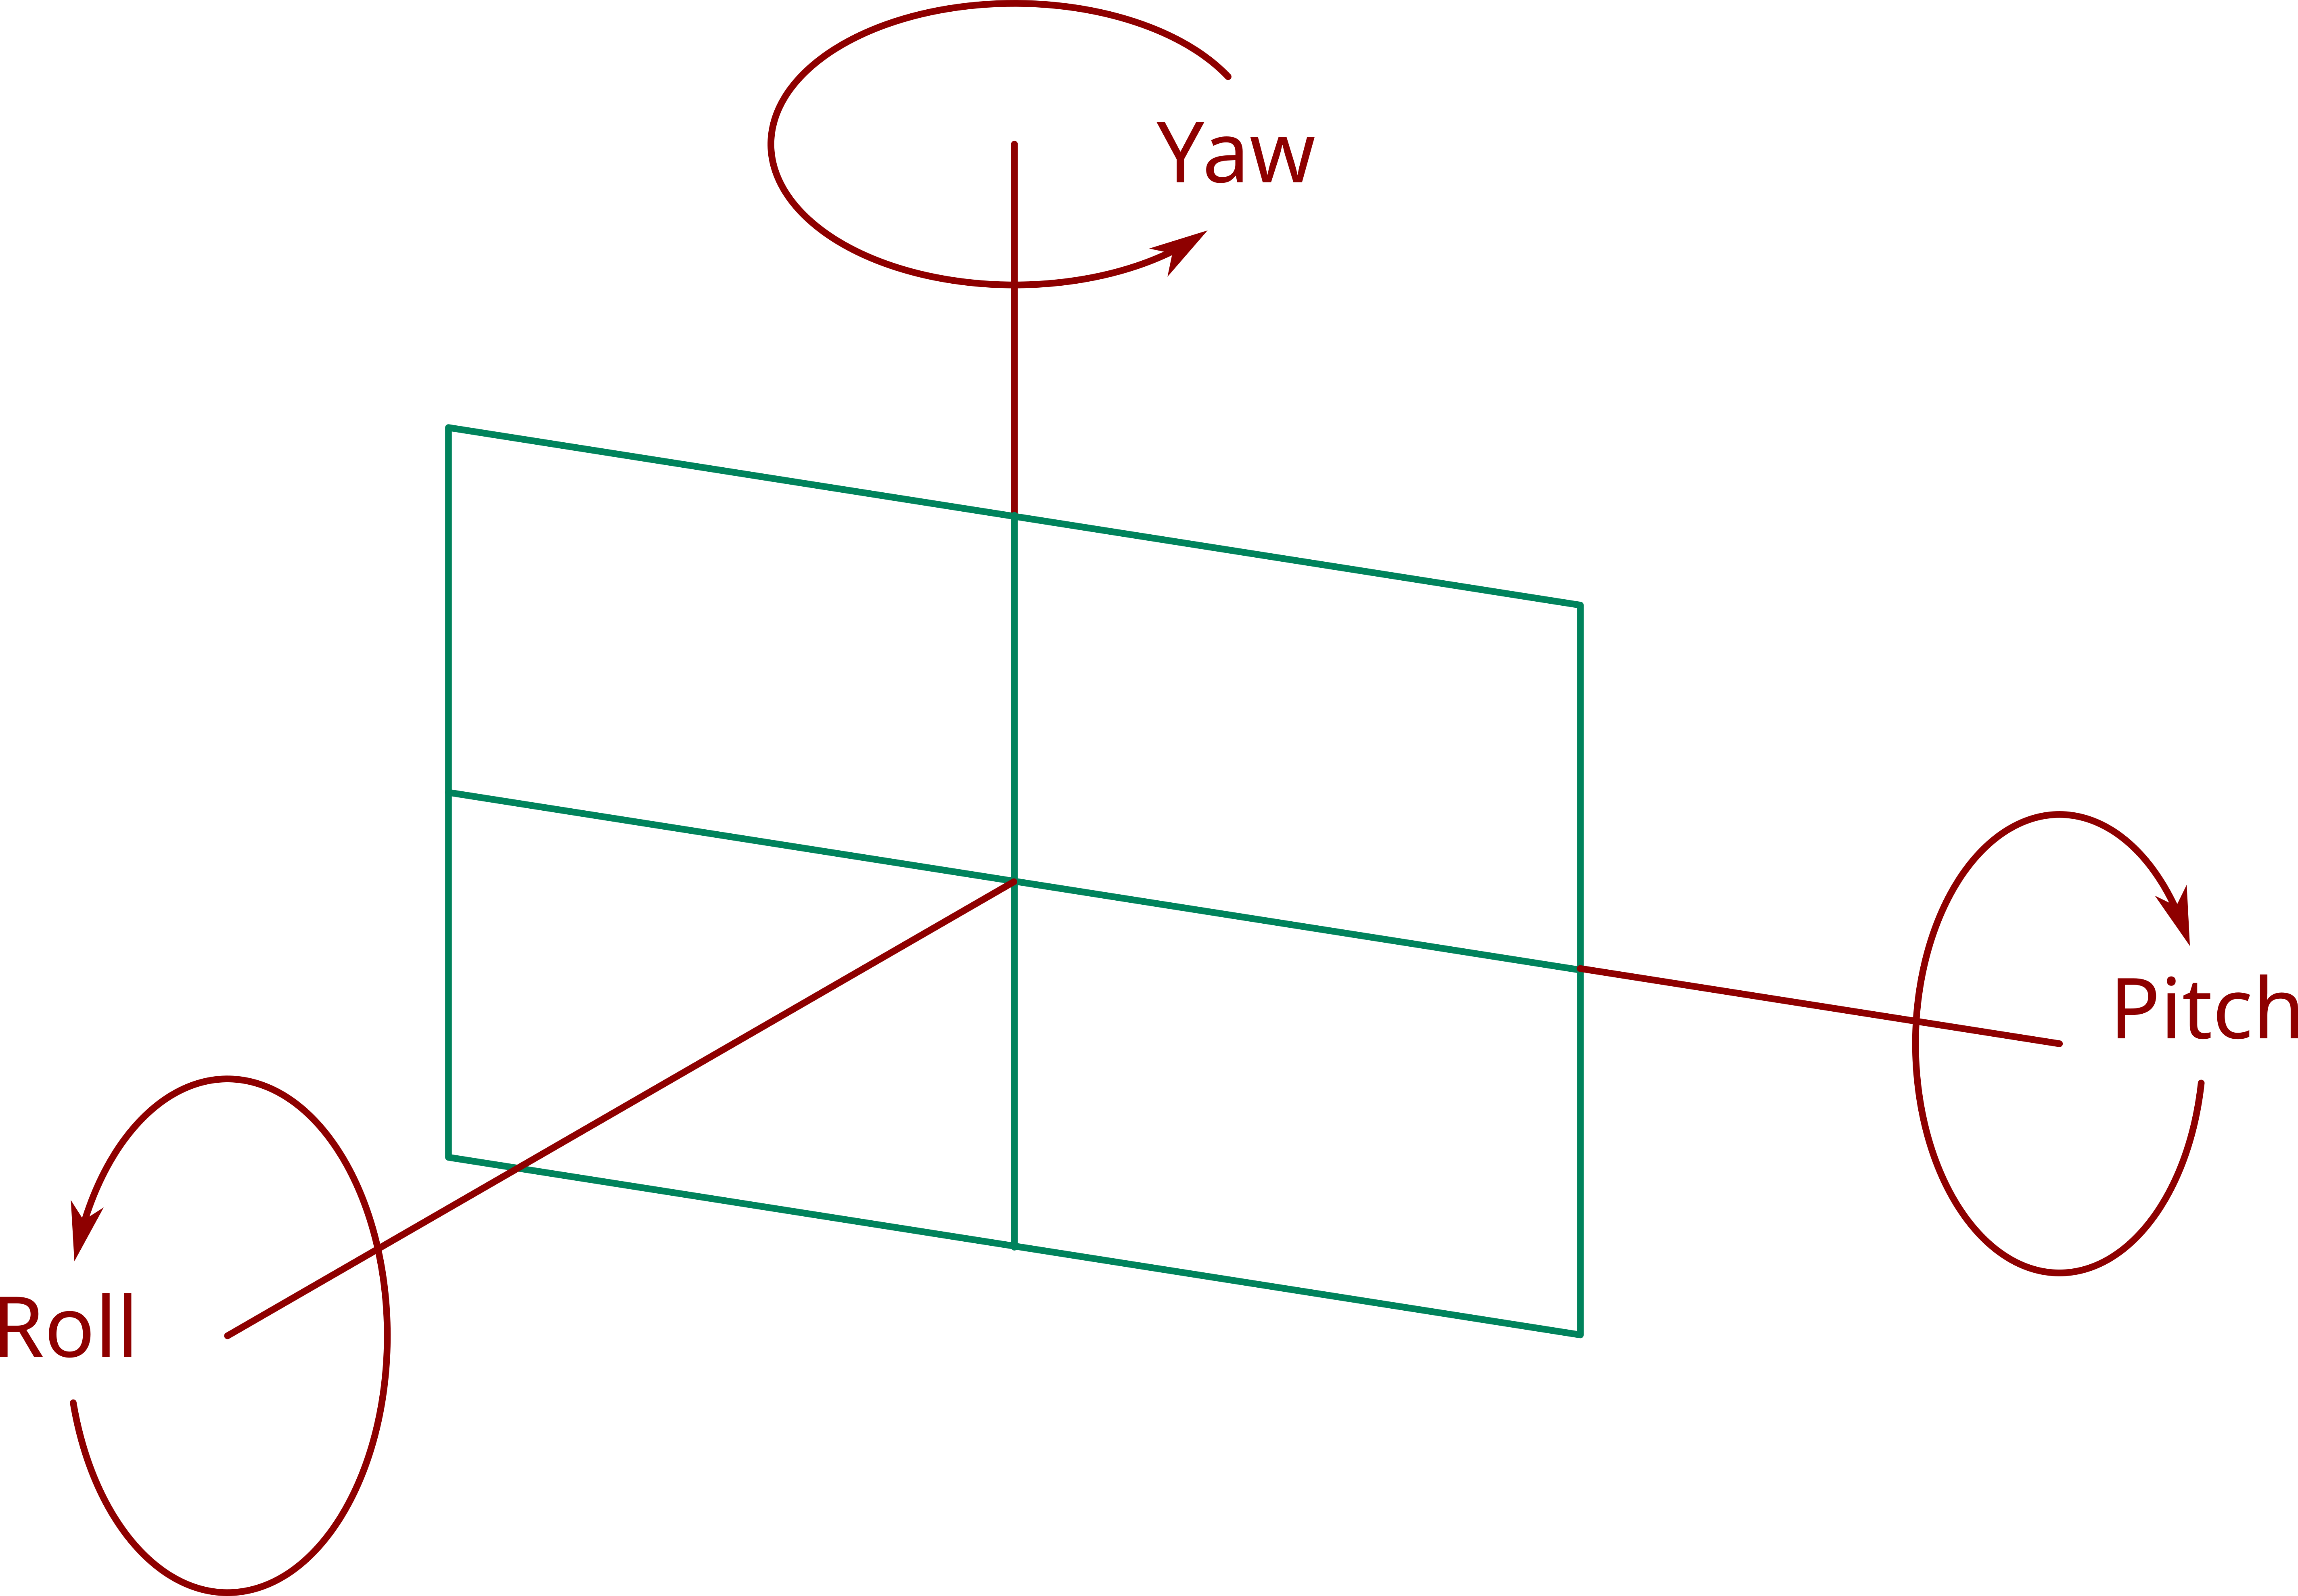
\includegraphics[width=.8\linewidth]{gfx/rollpitchyaw.png}
	\caption[Pitch, roll and yaw angles]{Pitch, roll and yaw angles}
	\label{fig:pitchrollyaw}
\end{figure}

This model let us compute the direction of the incoming rays just by indexing the particular pixel they hit, obtaining a map
\begin{equation}
\label{eq:pixelmap}
(p_x, p_y) \xmapsto{\mathfrak{h}_2} (\vartheta_{cs}, \varphi_{cs}),
\end{equation}
where $(p_x, p_y)$ are the components of the pixel in a system of coordinates whose origin is placed at the top-left corner of the sensor.

By composing \autoref{eq:initmap} and \autoref{eq:pixelmap}, we define the map
\begin{equation}
(p_x, p_y) \xmapsto{\mathfrak{h} = \mathfrak{h_1}\circ\mathfrak{h_2}} (\vartheta', \varphi'),
\end{equation}
that summarises all the work the algorithm does: from a pixel on the camera's reference frame, we compute the origin of the incoming ray that hit that pixel.

\subsubsection*{Pixel to Ray Map}
\label{subcsec:pixeltoray}

Let us consider a pixel $P$ whose coordinates on the sensor's reference frame are, in physical units, $(p_x, p_y)$, as depicted in \autoref{fig:pinhole}.

\begin{figure}[bth]
	\myfloatalign
	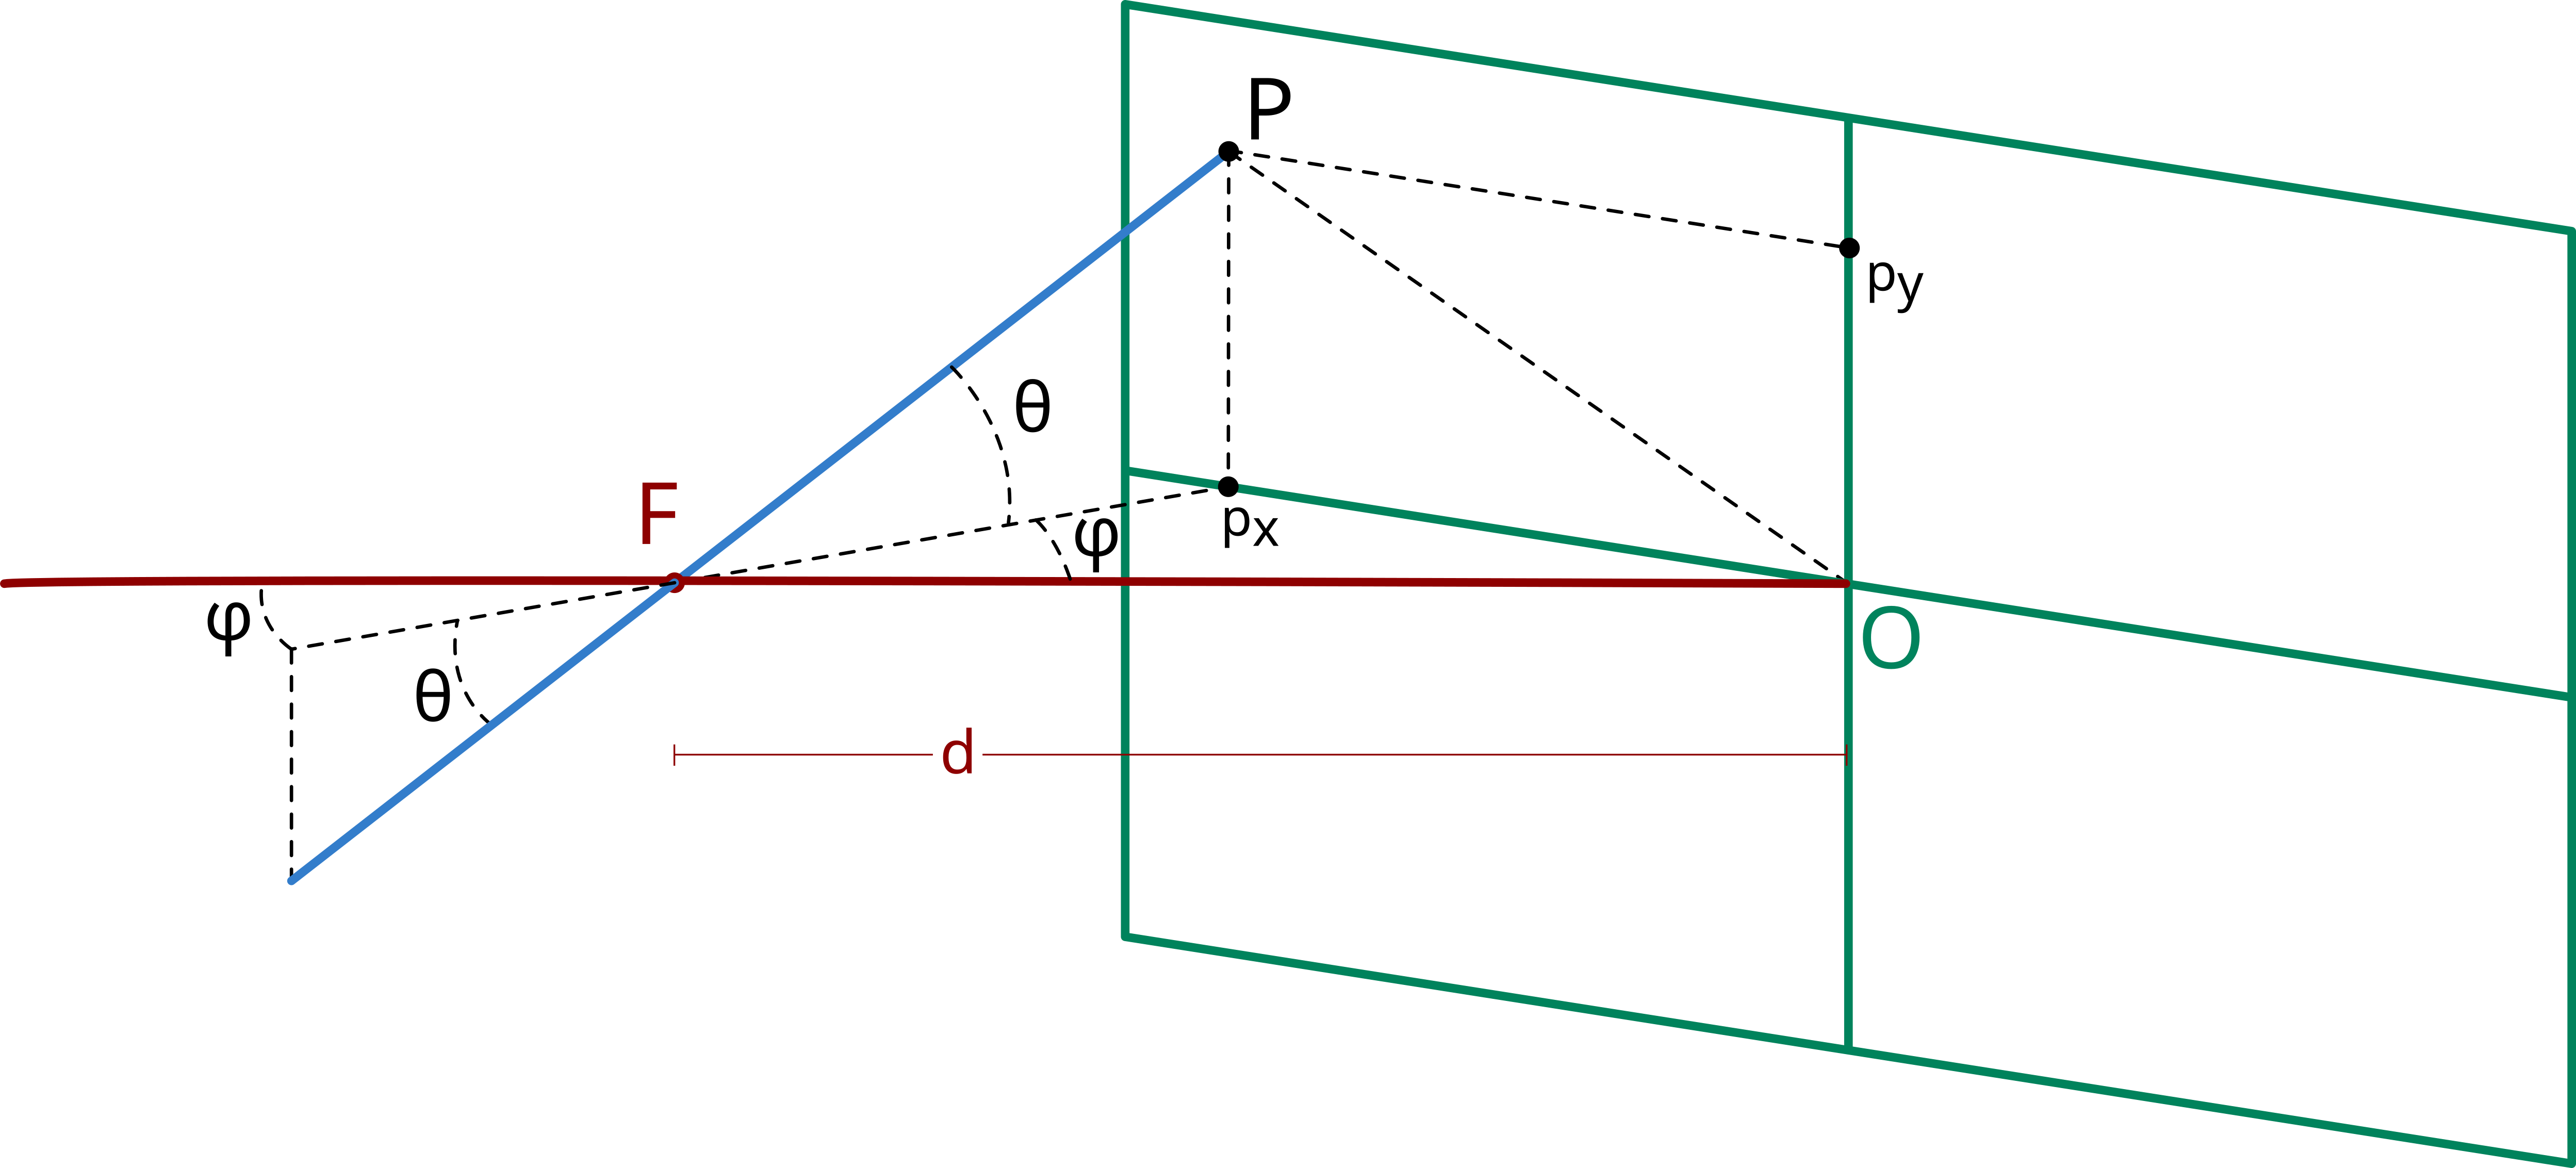
\includegraphics[width=.8\linewidth]{gfx/pinhole.png}
	\caption[Pinhole camera model]{Pinhole camera model}
	\label{fig:pinhole}
\end{figure}

All rays that hit the sensor are assumed, by our model, to pass through the focal point $F$. Thus, we can compute the angles $\vartheta$ and $\varphi$ for the ray hitting the sensor at pixel $P$ with elementary trigonometry.

From triangle $Fp_xO$ in \autoref{fig:pinhole}, we can obtain the angle $\varphi$ as
\[
\varphi = \arctan{\frac{p_x}{d}}.
\]

Similary, the value of $\vartheta$ comes from the triangle $Fp_xP$ in \autoref{fig:pinhole}, which results in the following formula:
\[
\vartheta = \arctan{\frac{p_y}{\sqrt{p_x^2 + d^2}}}.
\]

Finally, we need to adjust the zero for both $\vartheta$ and $\varphi$ to agree with the angle convention of the coordinate system. Therefore, the final formulas to computing the direction of an incoming ray hitting the camera's sensor as a pixel $P = (p_x, p_y)$ are the following:
\begin{align}
\vartheta_{cs} &= \frac{\pi}{2} + \arctan{\frac{p_y}{\sqrt{p_x^2 + d^2}}}, \\
\varphi_{cs} &= \pi + \arctan{\frac{p_x}{d}}.
\end{align}

This discussion assumed the pixel coordinates to have its origin at the centre of the sensor. This is not the common coordinate system for pixels, as it usually has its origin at the top-left corner. A simple translation fixes that.

Furthermore, the pitch, roll and yaw angles were assumed to be zero. However, the addition of these angles is not difficult:
\begin{itemize}
	\item The roll angle, noted as $\alpha$, defines the rotation of the sensor on the image plane, so every pixel $(p_x, p_y)$ has to be rotated accordingly:
	\[
	\begin{pmatrix}
	p'_x \\
	p'_y
	\end{pmatrix} = 
	\begin{pmatrix}
	\cos\alpha & -\sin\alpha \\
	\sin\alpha & \cos\alpha 
	\end{pmatrix}
	\begin{pmatrix}
	p_x \\
	p_y
	\end{pmatrix}.
	\]
	\item The pitch angle, noted as $\eta$, has to be simply added to the $\vartheta$ coordinate, as it defines the rotation of the sensor on that axis.
	\item The yaw angle, noted as $\lambda$, is the rotation of the sensor with respect to the $\varphi$ axis, so it has to be added to that coordinate.	
\end{itemize}

Taking all this into account, the final formulas to compute $(\vartheta_{cs}, \varphi_{cs})$ from the physical coordinates of the pixel $(p_x, p_y)$ are
\begin{align}
\label{eq:pinhole1}
\vartheta_{cs} &= \eta + \frac{\pi}{2} + \arctan{\frac{p_y}{\sqrt{p_x^2 + d^2}}}, \\
\label{eq:pinhole2}
\varphi_{cs} &= \lambda + \pi + \arctan{\frac{p_x}{d}},
\end{align}
where
\[
p'_x = p_x\cos\alpha - p_y\sin\alpha, \qquad
p'_y = p_x\sin\alpha + p_y\cos\alpha.
\]

\subsection{Initial Conditions Computation}
\label{sec:initcond}

The algorithm kernel integrates, backwards in time, an \ac{ODE} system. We already know the system we are working with, \autoref{theo:eqsmotion}, but for such a system to be uniquely solved, a set of initial conditions is needed.

That is, for each ray we need to know its components, \[(r, \vartheta, \varphi, p_r, p_\vartheta),\] at the time $\tau = 0$.

All rays hitting the camera share the same $r$, namely the position of the camera $r_c$.

In \autoref{subcsec:pixeltoray}, the initial $\vartheta_{cs}$ and $\varphi_{cs}$ for each ray were computed.

Therefore, we only need to compute the initial momentum components, $p_r$ and $p_\vartheta$, for each ray. In short, assuming we know the pixel the incoming ray is hitting and, thus, the $\vartheta_{cs}$ and $\varphi_{cs}$ components of the ray on the camera's local sky, we expect to obtain the map
\[
(\vartheta_{cs}, \varphi_{cs}) \xmapsto{IC} (p_r, p_\vartheta).
\]

This is not a difficult task but a very delicate one, as some coordinate systems have to be taken into account and we should have a good understanding of them in order to properly compute the bases changes. A short summary of the work that follows is listed here:
\begin{enumerate}
	\item The initial position of the ray is known to be $(r_c, \vartheta_{cs}, \varphi_{cs})$. The components of the unit vector that points on the direction of motion of the camera, $B$, are noted as $(B_{\widehat{r}}, B_{\widehat{\vartheta}}, B_{\widehat{\varphi}})$, whereas its speed relative to the \ac{FIDO}, that is, the modulus of $B$, is noted as $\beta$.
	\item From $(\vartheta_{cs}, \varphi_{cs})$ we compute the unit vector in Cartesian coordinates, $N = (N^x, N^y, N^z)$, pointing to the direction of the incoming ray. This is computed on the camera's reference frame: a simple change to Cartesian coordinates is needed.
	\item The relativistic aberration caused by the motion of the camera and its speed around the black hole causes the \ac{FIDO} to measure the direction of motion of the incoming ray slightly different. The Cartesian components of this derived unit vector, $n = (n^x, n^y, n^z)$ need to be computed.
	\item Then, $n_F$ needs to be seen from the \ac{FIDO}'s orthonormal basis by means of the ligatures provided by the vector $B$ and the orthogonal relations. This gives us the components $(n^r, n^\vartheta, n^\varphi)$.
	\item From $n_F$ expressed on the right coordinate system, we need to compute the covariant components of the four momentum $(p_t, p_r, p_\vartheta, p_\varphi)$.
\end{enumerate}

Before going ahead with the details of the five steps above, let us set up the bases on the vector spaces we are working on. First of all, for the spacetime written in \ac{BL} coordinates, $(t, r, \vartheta, \varphi)$, we have the usual basis for the tangent space $T_p M$,
\begin{equation}
\mathcal{B}_u = (\partial_t, \partial_r, \partial_\vartheta, \partial_\varphi).
\end{equation}

Furthermore, we would like to work with an orthonormal spherical basis, that will be noted as
\begin{equation}
\mathcal{B}_s = (e_t, e_r, e_\vartheta, e_\varphi).
\end{equation}

Finally, a Cartesian coordinate system placed on the camera's reference frame is needed. Its notation and components are:
\[
\mathcal{B}_c = (e_t, e_x, e_y, e_z).
\]

Let us now compute the expressions of the vectors in $\mathcal{B}_s$ in terms of the basis $\mathcal{B}_u$. We want an orthonormal basis, so for the spatial coordinates, it is only necessary to divide by its module. Therefore, their expressions in terms of $\mathcal{B}_u$ are:
\begin{equation}
e_r = \frac{\sqrt{\Delta}}{\rho} \partial_r, \quad
e_\vartheta = \frac{1}{\rho} \partial_\vartheta, \quad
e_\varphi = \frac{1}{\varpi} \partial_\varphi.
\end{equation}

For the time coordinate $e_t$ to be unitary and orthogonal to the spatial coordinates, we can define it as
\[
e_t = a\partial_t + b\partial_\varphi,
\]
where $a$ and $b$ are unknowns.

Imposing the orthonormality property ($e_t$ has to be negative unitary to preserve the signature and, in particular, $e_t$ is perpendicular to $e_\varphi$), we can set up a system of equations to solve $a$ and $b$:
\begin{align}
\label{eq:systemab}
g(e_t, e_t) &= -1, \\ \nonumber
g(e_t, e_\varphi) &= 0.
\end{align}

From \autoref{eq:systemab}, we conclude that $a = \frac{1}{\alpha}$ and $b = \frac{\omega}{\alpha}$. Therefore, the orthonormal basis $\mathcal{B}_s$ vectors are:
\begin{equation}
e_t = \frac{1}{\alpha}\partial_t + \frac{\omega}{\alpha}\partial_\varphi, \quad
e_r = \frac{\sqrt{\Delta}}{\rho} \partial_r, \quad
e_\vartheta = \frac{1}{\rho} \partial_\vartheta, \quad
e_\varphi = \frac{1}{\varpi} \partial_\varphi.
\end{equation}

The change of basis matrix, that maps $\mathcal{B}_s$ coordinates to $\mathcal{B}_u$ components is then
\begin{equation}
\mathcal{M} = \begin{pmatrix}
\frac{1}{\alpha} & 0 & 0 & 0 \\
0 & \frac{\sqrt{\Delta}}{\rho} & 0 & 0 \\
0 & 0 & \frac{1}{\rho} & 0 \\
\frac{\omega}{\alpha} & 0 & 0 & \frac{1}{\varpi}
\end{pmatrix}.
\end{equation}

This operation can be seen as an endomorphism on the tangent space, where we map vectors expressed in the orthonormal basis to vectors in the \ac{BL} coordinates. If we denote by $N$ the tangent space with the basis $\mathcal{B}_s$ and by $E$ the tangent space with the basis $\mathcal{B}_u$\footnote{Note that $N$ and $E$ are the same vector space, but their notations are different to express the different bases chosen.}, then $\mathcal{M}$ is the matrix of the endomorphism \[T \colon N \to E.\]

\subsubsection*{Incoming Ray Direction}

We can now begin with the first task: from the spherical coordinates of the ray on the camera's local sky, $(\vartheta_{cs}, \varphi_{cs})$, we can compute the Cartesian components of the unit vector $N = (N^x, N^y, N^z)$ that points in the direction of the incoming ray in the usual way:
\begin{equation}
N^x = \sin\vartheta_{cs} \cos\varphi_{cs}, \quad N^y = \cos\vartheta_{cs} \sin\varphi_{cs}, \quad N^z = \cos\vartheta_{cs}.
\end{equation}

\subsubsection*{Relativistic Aberration}

We have two observers: one local to the camera, that is measuring the ray's direction of motion as the vector $N$ and the \ac{FIDO}, which will see it as the vector $n = (n^x, n^y, n^z)$. As the camera moves at speed $\beta$, on the direction of $e_y$, with respect to the \ac{FIDO}, the Lorentz transformation can be written as
\begin{align}
\label{eq:lorentz}
dt' &= \frac{dt - \beta dy}{\upsilon}, \\ \nonumber
dx' &= dx, \\ \nonumber
dy' &= \frac{dy - \beta dt}{\upsilon}, \\ \nonumber
dz' &= d';
\end{align}
where $\upsilon = \sqrt{1 - \beta^2}$, $(dt', dx', dy', dz')$ are the \ac{FIDO} coordinates and $(dt, dx, dy, dz)$ are the coordinates local to the camera.

We can finally obtain the components $(n^x, n^y, n^z)$ just by applying \autoref{eq:lorentz}:
\begin{align*}
n^x &= \frac{dx'}{dt'} = \frac{\sigma dx}{dt - \beta dy} = \frac{\frac{dx}{dt} \upsilon}{1 - \beta \frac{dy}{dt}} = \frac{N^x \upsilon}{1 - \beta N^y}, \\
n^y &= \frac{dy'}{dt'} = \frac{dy - \beta dt}{dy}{dt - \beta dy} = \frac{N^y - \beta}{1 - \beta N^y}, \\
n^z &= \frac{dz'}{dt'} = \frac{\sigma dz}{dt - \beta dy} = \frac{\frac{dz}{dt} \upsilon}{1 - \beta \frac{dy}{dt}} = \frac{N^z \upsilon}{1 - \beta N^y}.
\end{align*}

The vector $N$ points in the direction of the incoming ray; particularly, it is pointing to the origin of the ray. The ray does not move \emph{to} its origin but \emph{from} there, so in order to have $n_F$ to point in the direction of motion of the ray, we must multiply $n$ by $-1$. This gives us the final equations for the relativistic aberration \cite[Eq. (A.9)]{thorne15}:
\begin{align}
n^x &= \frac{-\sqrt{1 - \beta^2}N^x}{1 - \beta N^y}, \\
n^y &= \frac{- N^y + \beta}{1 - \beta N^y}, \\
n^z &= \frac{-\sqrt{1 - \beta^2} N^z}{1 - \beta N^y}. \\
\end{align}

\subsubsection*{Change of Basis}

We have now the direction of the ray as seen by the \ac{FIDO} in the basis $\mathcal{B}_c$, but we want to express it in the spherical orthonormal coordinate system, whose basis is $\mathcal{B}_s$.

We need then to express one basis in terms of the other, using the orthonormality constraints and the direction of motion of the camera, $B$, whose coordinates are noted as $(B^r, B^\theta, B^\varphi)$.

First of all, we define $e_y$ to be $B$, so it is directly written in terms of the basis $\mathcal{B}_s$:
\begin{equation}
\label{eq:changey}
e_y = B^r e_r + B^\vartheta e_\vartheta + B^\varphi e_\varphi.
\end{equation}

We define $e_x$ to be perpendicular to $e_y$ and in the plane spanned by $e_r$ and $e_\varphi$, so we can write
\begin{equation*}
e_x = e_x^r e_r + e_x^\varphi e_\varphi,
\end{equation*}
where $e_x^r$ and $e_x^\varphi$ are the unknown coordinates. Using the orthonormality constraints, that is,
\begin{align*}
0 &= e_y e_x = B^r e_x^r + B^\varphi e_x^\varphi, \\
1 &= e_x e_x = \left( e_x^r \right)^2 + \left(e_x^\varphi\right)^2;
\end{align*}
we conclude that $e_x^r = \frac{B^\varphi}{\upsilon}$ and  $e_x^\varphi = -\frac{B^r}{\upsilon}$, so the $e_x$ component is written as
\begin{equation}
\label{eq:changex}
e_x = \frac{B^\varphi}{\upsilon} e_r - \frac{B^r}{\upsilon} e_\varphi.
\end{equation}

We proceed similarly to compute the spherical coordinates of $e_z$. Using the orhonormalization constraints, we have the system
\begin{align*}
0 &= e_y e_z = B^r e_z^r + B^\vartheta e_z^\vartheta + B^\varphi e_z^\varphi, \\
0 &= e_x e_z = \frac{B^\varphi}{\upsilon} e_z^r - \frac{B^r}{\upsilon} e_z^\varphi, \\
1 &= e_z e_z = \left(e_z^r\right)^2 + \left(e_z^\vartheta\right)^2 + \left(e_z^\varphi\right)^2,
\end{align*}
whose solution gives us the components of $e_z$:
\begin{equation}
\label{eq:changez}
e_z = \frac{B^r B^\vartheta}{\upsilon} e_r - \upsilon e_\vartheta + \frac{B^\vartheta B^\varphi}{\upsilon} e_\varphi.
\end{equation}

Using equations \ref{eq:changey}, \ref{eq:changex} and \ref{eq:changez}, it is then trivial to compute the components of $n$ in the spherical orthonormal basis $\mathcal{B}_s$:
\begin{align}
n^r &= \frac{B^\varphi}{\upsilon} n^x + B^r n^y + \frac{B^r B^\vartheta}{\upsilon} n^z, \\
n^\vartheta &= B^\vartheta n^y - \upsilon n^z, \\
n^\varphi &= \frac{B^r}{\upsilon} n^x + B^\varphi n^y + \frac{B^\vartheta B^\varphi}{\upsilon} n^z.
\end{align}

\subsubsection*{Momentum}

We finally have the direction of motion of the ray expressed in the proper basis, but in order to compute the initial conditions, we need its four momentum; that is, we want to obtain the function $f$ that maps $N$ to the dual space of $E$: $E^*$, as seen in \autoref{fig:diagram}, where $T$ is the endomorphism defined before and $\phi_N$, $\phi_E$ are the isomorphisms between the base spaces and their dual versions.

\begin{figure}[bth]
	\myfloatalign
	\begin{tikzpicture}
	\matrix (m) [matrix of math nodes,row sep=3em,column sep=4em,minimum width=2em]
	{
		N & E \\
		N^* & E^* \\};
	\path[-stealth]
	(m-1-1) edge node [left] {$\phi_N$} (m-2-1)
	edge [double] node [above] {$T$} (m-1-2)
	(m-2-2.west|-m-2-2) edge node [below] {$T^*$}
	(m-2-1)
	(m-1-2) edge node [right] {$\phi_E$} (m-2-2)
	(m-1-1) edge [right,dashed,->] node {$f$} (m-2-2);
	\end{tikzpicture}
	\caption[Conmutative diagram]{Conmutative diagram}
	\label{fig:diagram}
\end{figure}

Remember that $N$ has the orthonormal basis, so the expression of the metric on this space, noted as $\phi_N$, is trivial: its matrix is the diagonal $(-1, 1, 1, 1)$; \ie, only the sign of the time coordinate has to be changed. The expression of the metric on $E$, noted as $\phi_E$, is more difficult. That is why we are going to compute $f$ as
\begin{equation}
\label{eq:f}
f = (T^*)^{-1} \circ \phi_N,
\end{equation}
an not as $f = \phi_E \circ T$.

Using matrix notation, \autoref{eq:f} can be written as
\begin{equation}
\mathcal{M}_f = \left(\mathcal{M}^t\right)^{-1} \mathcal{M}_{\phi_N},
\end{equation}
where
\[
\left(\mathcal{M}^t\right)^{-1} = \begin{pmatrix}
\alpha & 0 & 0 & -\omega\varpi \\
0 & \frac{\rho}{\sqrt{\Delta}} & 0 & 0 \\
0 & 0 & \rho & 0 \\
0 & 0 & 0 & \varpi
\end{pmatrix}
\]
and
\[
\mathcal{M}_{\phi_N} = \begin{pmatrix}
-1 & 0 & 0 & 0\\
0 & 1 & 0 & 0\\
0 & 0 & 1 & 0\\
0 & 0 & 0 & 1
\end{pmatrix}.
\]

The moment of the ray is then $f(n)$, that is,
\begin{equation}
\begin{pmatrix}
p_t \\
p_r \\
p_\vartheta \\
p_\varphi \\
\end{pmatrix} = \begin{pmatrix}
-\alpha & 0 & 0 & -\omega\varpi \\
0 & \frac{\rho}{\sqrt{\Delta}} & 0 & 0 \\
0 & 0 & \rho & 0 \\
0 & 0 & 0 & \varpi
\end{pmatrix}
\begin{pmatrix}
1 \\
n^r \\
n^\vartheta \\
n^\varphi
\end{pmatrix} = \begin{pmatrix}
-\alpha - \omega\varpi n^\varphi \\
\frac{\rho}{\sqrt{\Delta}} n^r \\
\rho n^t \\
\varpi n^\varphi
\end{pmatrix}.
\end{equation}

We know that Kerr is stationary, so $p_t$ is conserved (see \autoref{eq:conservedpt}). We will normalize it by defining
\[
E_f = - \frac{1}{p_t}
\]  
as the energy measured by the \ac{FIDO} and multiplying $p$ by $E_f$. The final components of the momentum \cite[Eq. (A.11)]{thorne15} are:
\begin{align}
p_t &= -1, \\
p_r &= E_f \frac{\rho}{\sqrt{\Delta}} n^r, \\
p_\vartheta &= E_f \rho n^t, \\
p_\varphi &= E_f \varpi n^\varphi.
\end{align}

Because of the axial symmetry on Kerr black holes (see \autoref{eq:conservedpphi}), $p_\varphi$ is another conserved quantity. With this and the Carter's constant, defined at \autoref{eq:carter}, and using that the mass of the lightlike particles is zero and the energy is unitary, we can define the two ray's conserved quantities \cite[Eq. (A.12)]{thorne15}:
\begin{equation}
b \defeq p_\varphi, \quad q \defeq p_\vartheta^2 + \cos^2\vartheta \left( \frac{b^2}{\sin^2\vartheta} - a^2 \right).
\end{equation}

\subsection{Numerical Solver}
\label{sec:numerical}

Once we have the \ac{ODE} system and the initial conditions for the ray we want to solve, the final step is to numerically integrate, backwards in time, the geodesic followed by the ray.

The problem reduces then to numerically integrate an \ac{ODE} system, which is a well-known problem and widely studied in the literature.

In order to accomplish this task, the algorithm used by our ray tracer uses a classic \ac{RK} method, along with an automated step size computation based on the estimated error of the step.

The \ac{RK} method is based on the \texttt{DOPRI5} algorithm, described in \cite{hairer93} and \cite{hairer96}.

The automated control for the step size based on the estimated error follows the ideas in \cite[Sec. II.4, Subsec. Automatic Step Size Control]{hairer93}.

Furthermore, the step size is stabilized using the algorithm described in \cite[Sec. IV.2]{hairer96}.

\subsubsection*{Adaptive Runge-Kutta Method}

The \ac{RK} methods solve general \ac{IVP} like the following one,
\begin{align*}
\dot{y} = f(t,y) \\
y(t_0) = y_0,
\end{align*}
where $y$ can be scalar or vector and $f$, $t_0$ and $y_0$ are known.

Given a pair $(t_n, y_n)$, the adaptive \ac{RK} methods compute the value of the system at time $t_{n+1}$ as follows:
\begin{align*}
y_{n+1} = y_n + h \sum_{i=1}^s b_i k_i\\
y^*_{n+1} = y_n + h \sum_{i=1}^s b^*_i k_i,
\end{align*}

where $y_{n+1}$ is the new estimated value and $y^*_{n+1}$ is a higher order approximation that is used to estimate the error of the result, which is computed as $\vert y^*_{n+1} - y_{n+1} \vert$. In this notation, $h$ is the so-called \emph{step}, which is the amount of time the system is advanced, and the components $k_i$ are defined as follows:
\[
k_i = f(t_n + c_ih, y_n + h\sum_{j=1}^{i-1} a_{ij} k_j).
\]

The coefficients $a_{ij}$, $b_i$, $b_i^*$ and $c_i$ define the model, and are usually arranged on what is called a Butcher's table (see \autoref{tab:generalbutcher} for a generic example).

\begin{table}[bth]
	\myfloatalign
	\begin{tabularx}{.54\textwidth}{c|ccccc}
		$0$&  & & & & \\
		$c_2$& $a_{21}$ & & & & \\
		$c_3$& $a_{31}$ & $a_{32}$ & & & \\
		$\vdots$& $\vdots$ &  & $\ddots$ & & \\
		$c_s$& $a_{s1}$  & $a_{s2}$ & $\cdots$ & $a_{s(s-1)}$ & \\ \hline
		& $b_1$ & $b_2$ & $\cdots$ & $b_{s-1}$ & $b_s$ \\ \hline
		& $b^*_1$ & $b^*_2$ & $\cdots$ & $b^*_{s-1}$ & $b^*_s$ \\
	\end{tabularx}
	\caption[Butcher's table for an adaptive RK method]{Butcher's table for a generic adaptive \ac{RK} method.}
	\label{tab:generalbutcher}
\end{table}

Our system of \ac{ODE}, \autoref{theo:eqsmotion}, follows this model:
\begin{enumerate}
	\item $\dot{y} = (\dot{r}, \dot{\vartheta}, \dot{\varphi}, \dot{p}_r, \dot{p}_\vartheta)$,
	\item $f(t,y)$ is the right hand side of the equations and actually it does not depend on $t$, thus it can be written as $f(y)$.
	\item $t_0 = 0$ and $y_0 = (r_c, \vartheta_{cs}, \varphi_{cs}, p_{r}, p_{\vartheta})$ are the initial conditions computed in \autoref{sec:initcond}.
\end{enumerate}

The selected \ac{RK} algorithm is a fourth order method with an estimation of the error based on a fifth order approximation, and whose Butcher's table is described on \autoref{tab:butcher}.

\begin{table}[bth]
	\myfloatalign
	\begin{tabularx}{.9\textwidth}{c|ccccccc}
		$0$&  & & & & & & \\
		$\frac{1}{5}$&  $\frac{1}{5}$& & & & & & \\
		$\frac{3}{10}$&  $\frac{3}{40}$&  $\frac{9}{40}$& & & & & \\
		$\frac{4}{5}$&  $\frac{44}{45}$&  $-\frac{56}{15}$&  $\frac{32}{9}$& & & & \\
		$\frac{8}{9}$&  $\frac{19372}{6561}$&  $-\frac{25360}{2187}$&  $\frac{64448}{6561}$&  $-\frac{212}{729}$& & & \\
		$1$&  $\frac{9017}{3168}$&  $-\frac{355}{33}$&  $\frac{46732}{5247}$&  $\frac{49}{176}$&  $-\frac{5103}{18656}$& & \\
		$1$&  $\frac{35}{384}$&  $0$&  $\frac{500}{1113}$&  $\frac{125}{192}$&  $-\frac{2187}{6784}$&  $\frac{11}{84}$& \\ \hline
		$y_1$&  $\frac{35}{384}$&  $0$&  $\frac{500}{1113}$&  $\frac{125}{192}$&  $-\frac{2187}{6784}$&  $\frac{11}{84}$&  $0$ \\ \hline
		$\widehat{y}_1$&  $\frac{5179}{57600}$&  $0$&  $\frac{7571}{16695}$&  $\frac{393}{640}$&  $-\frac{92097}{339200}$&  $\frac{187}{2100}$&  $\frac{1}{40}$
	\end{tabularx}
	\caption{Butcher's table for the ray tracer solver}
	\label{tab:butcher}
\end{table}

\subsection{Accretion Disk}

Accretion disks are disk-like structures, usually made of gas or dust, orbiting around massive objects, such as the black holes we are dealing with.

The design of the ray tracer has taken this into account, including a feature that provides the user with the possibility of adding an infinitely thin accretion disk orbiting on the equatorial plane.

This disk, always placed on the equatorial plane and that shares its centre with the black hole's, is defined as an annulus characterised by its inner and outer radii, denoted as $r_{in}$ and $r_{out}$.

The interaction between the geodesics and the accretion disk is really interesting to see the distortion in the spacetime near the shadow. It is then mandatory to have a way of detecting if an integrated geodesic collides with the disk.

The only way of detecting this collision is continuously checking if the geodesic has crossed the equatorial plane. If the geodesic is on the equatorial plane, \ie, if its $\vartheta$ coordinate is equal to $\nicefrac{\pi}{2}$, it is in collision with the disk if, and only if, its $r$ coordinate satisfies
\begin{equation}
\label{eq:collision}
r_{out} > r > r_{in}.
\end{equation}

The solver works with discrete time intervals, \ie, we know the value $y(t_0)$ and it can compute the value $y(t_1)$. Therefore, it is probable that if a geodesic crosses the equatorial plane, it does it at a time $t \in (t_0, t_1)$. The only way of assuring that we detect the equatorial plane crossing, is to look at the change of the sign of $\vartheta$ with respect to $\nicefrac{\pi}{2}$ at the edges of the interval. That is, we know that a geodesic crosses the equatorial plane in an interval $[t_0, t_1]$ if and only if $\vartheta(t_0) < \nicefrac{\pi}{2}$ and $\vartheta(t_1) \geq \nicefrac{\pi}{2}$, or the other way around.

\subsubsection*{Bisection Algorithm}

With this constraint in mind, it is necessary to design a way of computing the exact point where a geodesic crosses the equatorial plane. A bisection algorithm is the solution proposed: when we detect that a geodesic crosses the equatorial plane in an interval $[t_0, t_1]$, we ask the solver to compute whether it crossed it in the interval $[t_0, \nicefrac{(t_1 - t_0)}{2}]$. If the answer is affirmative, we repeat the process by changing $t_1 = \nicefrac{(t_1 - t_0)}{2}$; otherwise, we make the check assuming $t_0 = \nicefrac{(t_1 - t_0)}{2}$. The process repeats until a pre defined error tolerance, or a pre defined maximum number of iterations, is reached. This usual bisection technique let us find the exact point where the crossing took place, and let us check whether the geodesic satisfies \autoref{eq:collision} when $\vartheta \approx \nicefrac{\pi}{2}$.

The first design assumed the collision detection and the \ac{RK} solver to be independent tasks. That is, the ray tracer called the solver several times with very small time intervals in order to check, between these calls, whether the geodesic has collided with the disk.

\begin{algorithm}
	\caption{Disk collision detection - rejected version}
	\label{alg:collision}
	\begin{algorithmic}[1]
		\Function{Collision Detection}{resolution}
		\For{$t$ from $t_0$ to $t_{end}$ in steps of size resolution}
		\State RKSolver(t, t + resolution)
		\If{the geodesic has crossed the eq. plane}
		\State collisionCheck $\gets$ bisection($[t, t + resolution]$)
		\EndIf
		\EndFor
		\Return{collisionCheck}
		\EndFunction
	\end{algorithmic}
\end{algorithm}

This idea, depicted on \ref{alg:collision}, caused a great loss on the efficiency ---we were artificially bounding the step size computed by the automatic step algorithm---, as well as the addition of the parameter resolution, which changed the final performance greatly. This was difficult and a bad design decision, so the solution was redesigned. The final idea, that was then proved to be very efficient, consisted on assimilating the collision detection inside the solver itself.

That way, the \ac{RK} solver is called only once, with the final time interval $[t_0, t_{end}]$. The resolution variable is removed, as it is the same solver, with its automatic step size detection, who decides when to call the check and the bisection.

















\section{Solution Implementation}
\label{chapter:implementation}

This chapter covers the implementation details, the technologies used, the different decisions made and the reasons that led us to make them.

In short, the software developed is a Python package that implements a general relativity ray tracer using the library \ac{CUDA} as the back-end, generating images of a Kerr black hole from close distances.

The primary requirement when designing and implementing the software has been the \emph{ease of use}. The Python package exposes a minimal yet powerful public \ac{API}, abstracting all \ac{CUDA}-related code and letting the user configure the properties of the black hole and the cameras placed near it.

\subsection{Technologies Used}

The base code, exposed to the final user and with an easy to understand \ac{API}, is written in Python. The reason to choose this language is that it is widely used in the scientific community, and whose rise on these fields is increasing. Furthermore, it let us write simple understandable code withouth losing the power of the \ac{OOP}.

The \ac{CUDA} code is written in \ac{CUDA}-C, an extension of the well-known C language that permits to manage the \ac{GPU} and to establish a communication between the host (the \ac{CPU}) and the device (the \ac{GPU}). This is the most difficult code, highly optimised and where the ray tracer kernel and \ac{RK} solver are implemented.

In order to glue together the Python package and the \ac{CUDA} kernel, the PyCUDA library is used.

Finally, Sphinx has been used to manage the documentation of the package, letting the user access the Python docstrings on the objects defined. The C code has been documented using Doxygen, whose output is takes as an input by Sphinx in order to generate a complete documentation.

\subsubsection*{Python Package}

The Python package is organised in four main files:
\begin{enumerate}
	\item \lstinline{universe.py}: defines a \lstinline{Universe} class, and exposes an instance of it to the package. This instace, called \lstinline{universe}, has all the general information about the spacetime, namely the black hole's spin and the accretion disk radius.
	\item \lstinline{camera.py}: defines a \lstinline{Camera} class, that contains all the necessary information that characterise it: the sensor size in physical units, the sensor resolution, the roll, pitch and yaw angles and its position with respect to the black hole centre. Internally, the \lstinline{Camera} class has an attribute called \lstinline{engine}, which is an instance of the \lstinline{RayTracer} class. The \lstinline{Camera} class is in charge of computing the $\alpha$, $\omega$ and $\varpi$ quantities, that defines the value of the Kerr metric on the point where the camera is placed.
	\item \lstinline{raytracer.py}: defines a \lstinline{RayTracer} class, which implements the PyCUDA calls to the \ac{CUDA} kernels. From the user perspective, it is the class that solves the \ac{ODE} system, although it delegates this work on the \ac{CUDA} methods.
	\item \lstinline{geodesics.py}: defines a main \lstinline{Congruence} class, which is a set of solved geodesics with their position at every computed time. There are two more classes defined in this file: \lstinline{GeodesicSnapshot}, which is a slice of the \lstinline{Congruence} containing the position of all computed geodesics at a single instant and \lstinline{Geodesic}, which is a slice of \lstinline{Congruence} containing one single geodesic with its position at all computed times.
\end{enumerate}

The workflow when using this package as a user would be: import the \lstinline{universe} instance and the \lstinline{Camera} class from the package, define as much cameras as desired and configure their properties, configure the spin of the black hole and the accretion disk through the \lstinline{universe} instance if the default values are not wanted and call the method \lstinline{shoot()} from an instance of the camera. This returns a \lstinline{CongruenceSnapshot} instance that can be plotted with its method \lstinline{plot()}.

\subsubsection*{CUDA}

All \ac{CUDA} related files are stored in a directory inside the package. There are four main files inside that directory:
\begin{enumerate}
	\item \lstinline{raytracer.cu}: defines two kernels, \lstinline{setInitialConditions} and \lstinline{kernel}. They are explained with detail in \autoref{sec:cuda}.
	\item \lstinline{solvers.cu}: implements the \ac{RK} solver along with the automatic step size computation algorithm.
	\item \lstinline{image_transformation.cu}: defines a third kernel, \lstinline{generate_image}, that manages the texture maps. See \autoref{sec:cuda} for more details.
	\item \lstinline{functions.cu}: implements the right hand side of the \ac{ODE} system; \ie, the $f(y)$ function.
\end{enumerate}

\subsubsection*{PyCUDA}

The interface between Python and \ac{CUDA} is implemented in the Python class \lstinline{RayTracer}. This class uses the PyCUDA module to configure the device, to manage the memory transactions between host and device and to execute the kernels on the device when the user on the host requests it.

\subsubsection*{Documentation: Sphinx and Doxygen}

The documentation of the software has been made with Sphinx on the Python code and with Doxygen in the C code.

This let us set up a workflow where we document the objects and methods and then we generate different outputs. For example, Sphinx can render HTML documents, and a web page was designed in order to publish a good documentation that can be consulted from everywhere. This web page is not finished, and it is not included in the final code, but \autoref{fig:screenshot} shows an example screenshot of what it looks like.

\begin{figure}[bth]
	\myfloatalign
	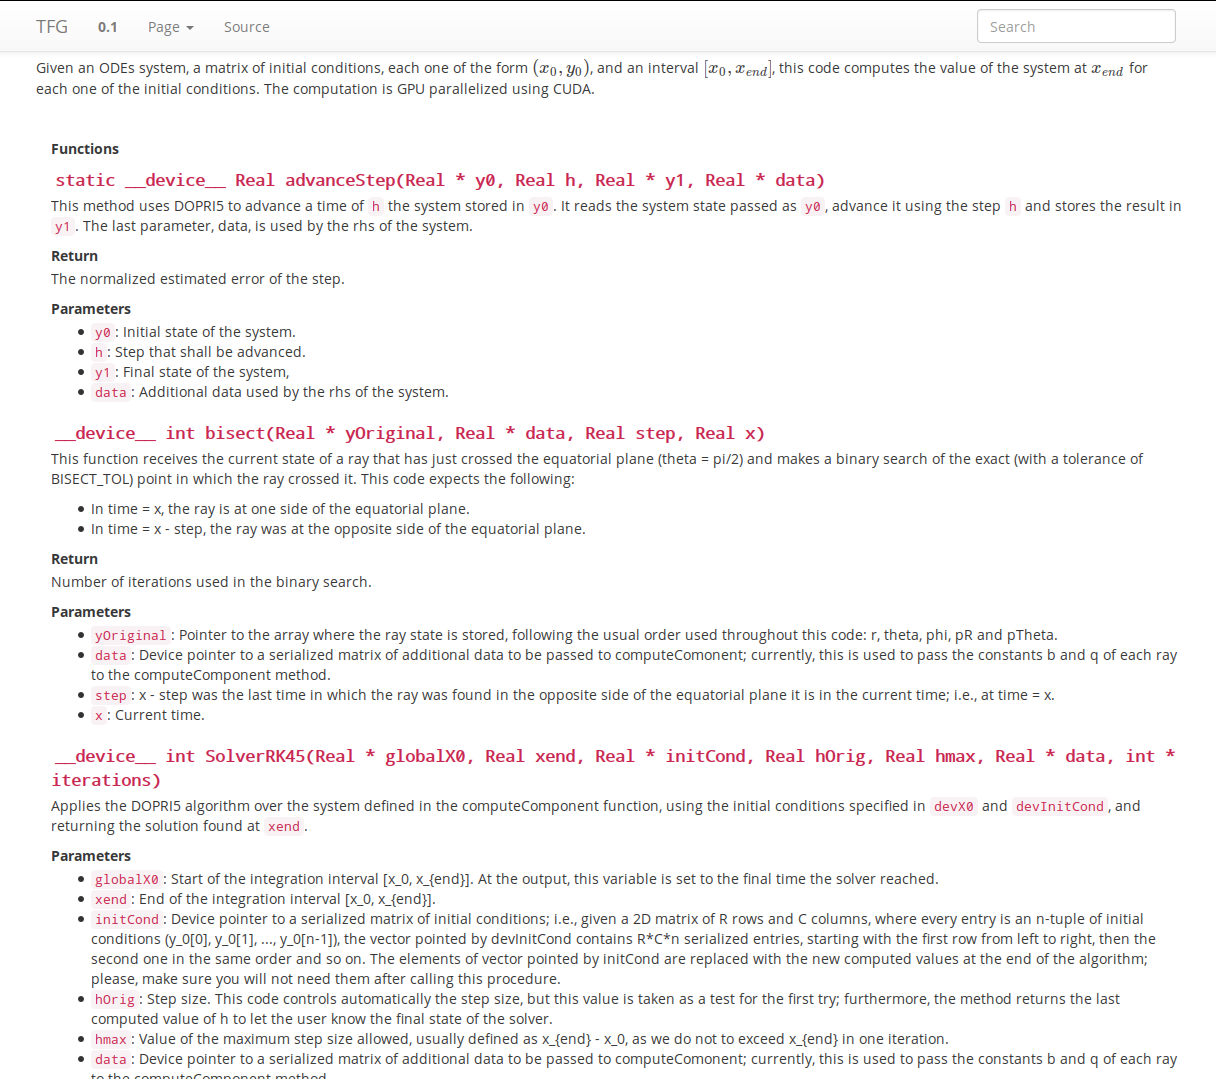
\includegraphics[width=\linewidth]{gfx/documentationscreenshot}
	\caption[Screenshot of the still unfinished web page]{Screenshot of the still unfinished web page.}
	\label{fig:screenshot}
\end{figure}

\subsection{Algorithm Implementation}

This section covers the implementation details for some of the most complex blocks on the code.

\subsection{CUDA Parallelization}
\label{sec:cuda}

\ac{CUDA} is a powerful library that abstracts the interaction with the \ac{GPU} in order to let the user implement general purpose programs on it.

\ac{CUDA} abstracts all kinds of \acp{GPU} in a hierarchy to manage instructions and shared memory. A list with the main levels on the hierarchy follows:
\begin{itemize}
	\item \emph{Thread}: the minimal unit managed by the \ac{GPU}. It is a set of data and instructions that is handled by a single processing unit of the \ac{GPU}. It has its own local memory, the fastest of all the memories defined by \ac{CUDA}, and is only accessible by the thread itself.
	\item \emph{Warp}: a logical set of 32 threads that execute the same instruction at the same time on different data. Although the consideration of the warps can be omitted by developers, a good design that takes this into account can increase the performance highly, as a warp takes advantage of the spatial locality of data, optimising accesses to memory.
	\item \emph{Block}: a three dimensional (although one can omit any of the dimensions) matrix where every element is a thread. All threads in a block can access a section of the memory, called \emph{shared memory}, which is much faster than the global memory. Every thread has a unique per-block identifier.
	\item \emph{Grid}: a three dimensional (although one can omit any of the dimensions) matrix where every element is a block. The memory accessible by all threads in all blocks is called the \emph{global memory}, and it is the slowest one. Every block has a unique identifier within the grid.
\end{itemize}

The \ac{CUDA} device is configured once at the beginning of the program as a set of threads, uniquely identified by their block indices and thread indices relative to the blocks.

\begin{figure}[bth]
	\myfloatalign
	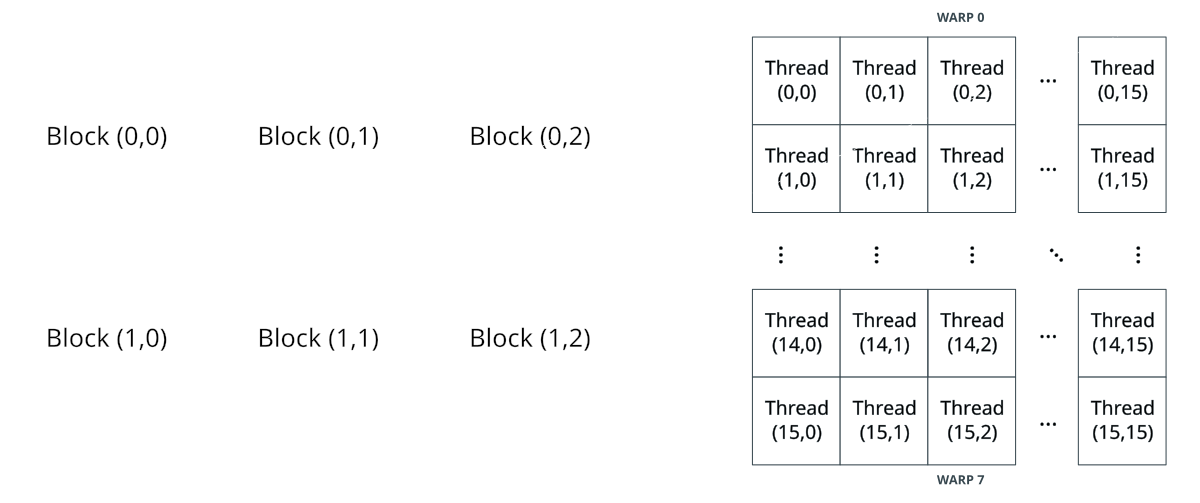
\includegraphics[width=.8\linewidth]{gfx/cudagrid}
	\caption[$2\times3$ grid with $16\times16$ blocks]{$2\times3$ grid with $16\times16$ blocks}
	\label{fig:cudagrid}
\end{figure}

An example configuration of the \ac{CUDA} device can be seen on \autoref{fig:cudagrid}, where 6 two dimensional blocks are arranged on the grid in two rows and three columns. Every block has 256 threads, arranged on a 16$\times$16 matrix.

The shape of the \ac{CUDA} grid and blocks are customizable by the user, but the warps are automatically created by \ac{CUDA}, picking up always sets of successive 32 threads, going first through the $X$ axis, then through the $Y$ axis and finally through the $Z$ axis.

This section will study how the grid and blocks are shaped on our software and the implemented parallelized code, as well as some fine-tuning techniques used to speed up the computations.

\subsubsection*{Device Setup}

The configuration of the grid for a ray tracer seems natural. As we are working with images, which are simply two dimensional matrices, the grid will be shaped as a two dimensional matrix, where every thread will compute the geodesic corresponding to a pixel.

The important question now is how to configure the pixels between the blocks; \ie, how to define the number of blocks per column and per row in the grid.

The simplest answer is to define one dimensional blocks of a fixed size that extend along the rows of the image. The very first implementation of the ray tracer used this configuration, but the speed up against the \ac{CPU} implementation was very poor.

The branch divergence was guilty of the poor performance: along a row of the image, the behaviour of the corresponding geodesics is very different, and the so-called \emph{warp divergence} occurs: in a warp, which in this configuration is defined along the rows of the image, all threads execute the same instruction at the same time; if the control flow varies between the threads in a warp, some of them will be idle, which causes a great loss of parallel efficiency.

This is avoided by designing a configuration that ensures, or at least that facilitates, that all the threads in a warp execute the same exact code without branch divergence. In our case, this means that the geodesics hitting the pixels in a warp should have followed a nearby path.

However, without knowing a priori the origin of the geodesics, we can only guess which pixels will have similar geodesics. The configuration design follows then this sensible guess: \emph{nearby pixels are hit by geodesics with nearby origins}.

From this assumption, we designed warps as squared as possible, configuring the blocks to have an integer number of warps. This resulted in the following configuration:
\begin{enumerate}
	\item Each block has $8\times8$ threads; \ie, two warps of $8\times4$ threads are located per block. See \autoref{fig:warpconf}.
	\begin{figure}[bth]
		\myfloatalign
		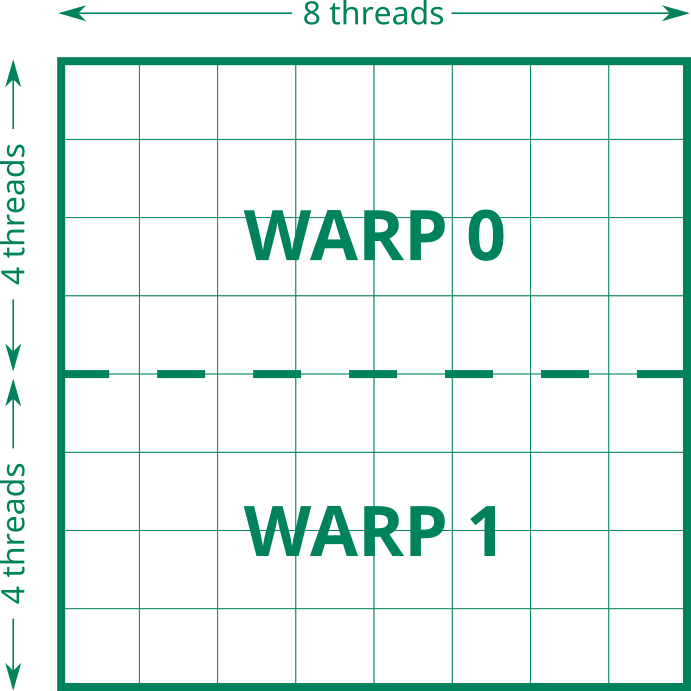
\includegraphics[width=.5\linewidth]{gfx/warpconf.png}
		\caption[Raytracer block configuration]{Raytracer block configuration}
		\label{fig:warpconf}
	\end{figure}
	\item The grid size is dynamically computed using the image size provided by the user. The number of rows and columns of the grid are computed with the following formulas:
	\begin{equation*}
	G_C = \left \lfloor{\frac{I_C - 1}{B_C} + 1}\right \rfloor, \qquad
	G_R = \left \lfloor{\frac{I_R - 1}{B_R} + 1}\right \rfloor,
	\end{equation*}
	where $G_C$ and $G_R$ are the number of blocks per column and per row, $I_C$ and $I_R$ are the columns and rows of pixels of the image and $B_C = B_R = 8$ are the number of columns and rows of a block. These formulas ensure we have enough threads to compute each pixel. The remaining threads, which do not have any geodesic to compute, will be idle during all the program execution.
\end{enumerate}

\subsubsection*{CUDA Kernels}

The main function executed by \ac{CUDA} on the \ac{GPU} is called the \emph{kernel}. Our implementation has three kernels, where every thread is identified with a pixel via its unique identifier in the \ac{CUDA} device. The kernels are:
\begin{enumerate}
	\item \lstinline{setInitialConditions()}: it is the kernel to compute the initial conditions for every pixel, as designed in \autoref{sec:initcond}. From the pixel coordinates, it computes the corresponding pair $(\vartheta_{cs}, \varphi_{cs})$.
	\item  \lstinline{kernel()}: it is the main kernel. It receives the initial conditions for every pixel and the final time until which the \ac{ODE} system will be integrated. It computes the origin of each geodesic, \ie, the pair $(\vartheta', \varphi')$, using the design described at \autoref{sec:numerical}, while continuously checking for collisions with the accretion disk.
	\item \lstinline{generate_image()}: it is an auxiliary kernel to map textures into the images. It receives the origin of the geodesic corresponding to each pixel in the image and maps it to a pixel in the provided texture.
\end{enumerate}

\subsubsection*{Optimizations}

The computational bottleneck of the ray tracer is the \ac{ODE} solver. In particular, the computation of the right hand side of the system ---in terms of the \autoref{sec:numerical}, the function $f(y,t)$---, which involves a lot of operations, some of them really expensive, as the \lstinline{sin()} and \lstinline{cos()} functions.

This chunk of code has been highly optimised, pre-computing all repeated operations and using efficient implementations such as the \lstinline{sincos()} function. The derivatives on equations \ref{eq:eqsmotionp}, \ref{eq:eqsmotionpr} and \ref{eq:eqsmotionpt} have been expressed in their most elementary terms and all common quantities between them have been also pre-computed. To optimise the memory access time, the thread's local memory has been used whenever it was possible.

Furthermore, a specific issue has been taking into account: the \ac{ILP}. It is clear that a single thread cannot keep the \ac{GPU} busy, so the device schedules threads and instructions in such a way that the \ac{GPU} is always busy.

One way of helping the \ac{CUDA} scheduler to maximize the device occupancy is to design the code optimising the \ac{ILP}. For example, imagine the following three lines of code:

\begin{lstlisting}
int rho = a + b;
int theta = c + d;
int m = rho * theta;
\end{lstlisting}

It is clear that the third one depends on the other two to be executed. However, the first two lines can be run in parallel. The scheduler then can run these two operations on different processor in order to speed up the computation.

All the ray tracer implementation is coded in such a way that independent instructions are together, whereas dependent ones are as far as possible one of the other. This let the scheduler issue instructions in parallel without having to wait for dependent computations to finish.

In particular, the code of the computation of $f(y,t)$ has been deeply studied in order to maximize the \ac{ILP}.

\subsubsection*{Initial Conditions Computation}

The initial conditions computation is implemented as a kernel on the \lstinline{raytracer.cu} file.

It receives a pointer to two allocated sections of memory in the device: one to store the output of the initial conditions and another to store the output of the computation of the conserved quantities $b$ and $q$.

Each thread solve the formulas obtained in \autoref{sec:pinhole}: equations \ref{eq:pinhole1} and \ref{eq:pinhole2} and the ones obtained in \autoref{sec:initcond}, and store the computed values in the pointed sections of the memory.

\subsubsection*{Ray Tracing}

The ray tracing kernel implements the main logic of the software: it executes the \ac{RK} solver while continuously checking for collisions with either the disk or the black hole, following the design on \autoref{sec:numerical}.

It receives a pointer to an allocated section of the memory where the initial conditions of the system are stored. After solving the \ac{ODE} system, it rewrites this buffer to provide the user with the final \ac{BL} coordinates of the considered geodesics.

An auxiliary buffer is used in order to known if a given geodesic has hit the disk, has fallen into the black hole or if it points to the celestial sphere.

\subsubsection*{Texture Mapping}

The texture mapping is a simple kernel implemented in the \lstinline{image_transformation.cu} file. It receives the final computed solution of the \ac{ODE} system, a pointer to a section of the memory where the textures pixels are assumed to be stored along with the size of the textures and a pointer to another previously allocated section of memory where the final pixels of the image will be stored.

It then computes the texture mapping and outputs the result to the final image.




















\section{Results}
\label{chapter:results}

The implemented software fulfils the objectives and requirements set at the design stage. It can ray trace arbitrary geodesics from the point of view of a camera, arbitrarily placed on a Kerr spacetime, allowing the user to plot the simulated geodesics both as photographies and as three dimensional projections.

\begin{figure}[bth]
	\myfloatalign
	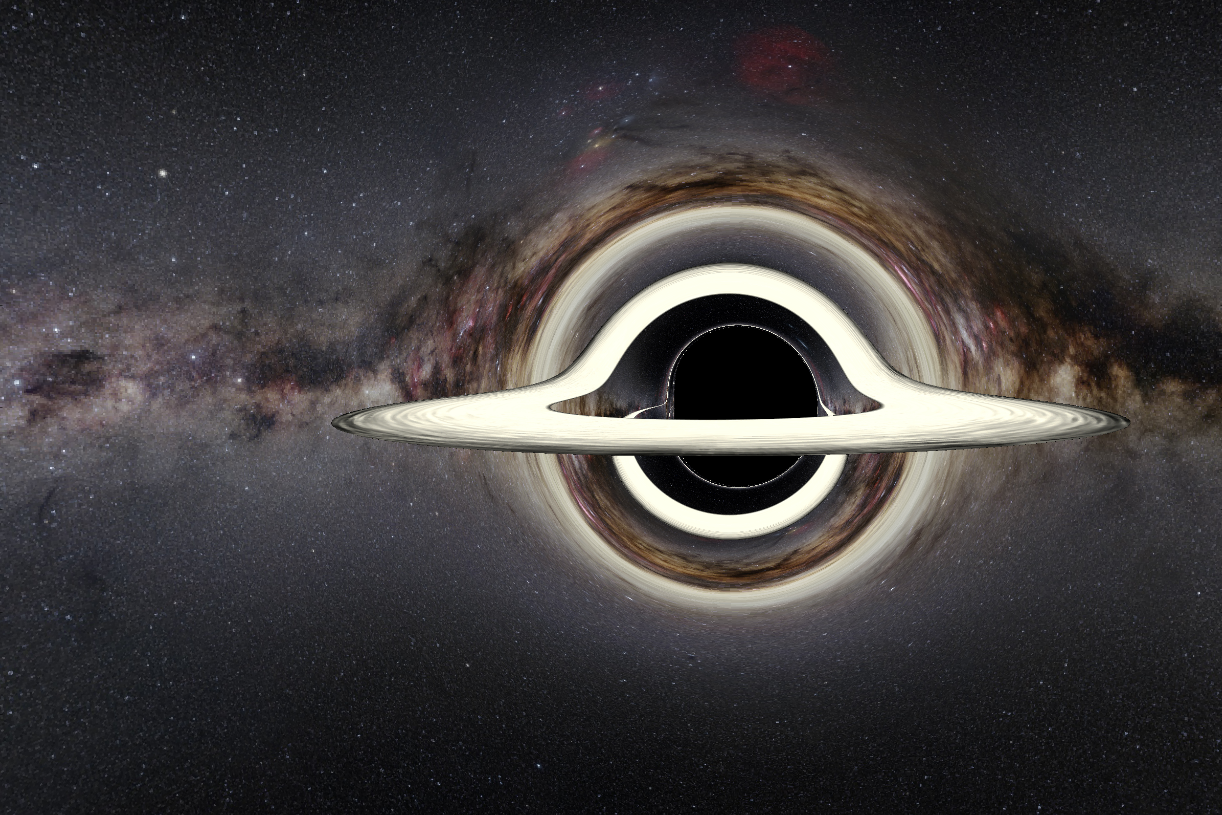
\includegraphics[width=\linewidth]{gfx/bh_texture_disk}
	\caption[Cinematographic textured image]{Cinematographic textured image}
	\label{fig:blackhole}
\end{figure}

Furthermore, the implemented \ac{ODE} solver accuracy was successfully tested, while the speed up of the \ac{GPU} parallelized code was proved to be very high.

\subsection{Ray Tracer Features}

The ray tracer generates images with a wide range of possibilities. First of all, it can render images that simulate photographies made with a common camera near the black hole. An accretion disk can be added to the black hole, showing the curvature of the light near its surroundings. For both the disk and the celestial sphere, arbitrary textures can be added, letting the user experiment with the light and the distortions produced by the greatly curved spacetime near the Kerr black hole.

\begin{figure}[bth]
	\myfloatalign
	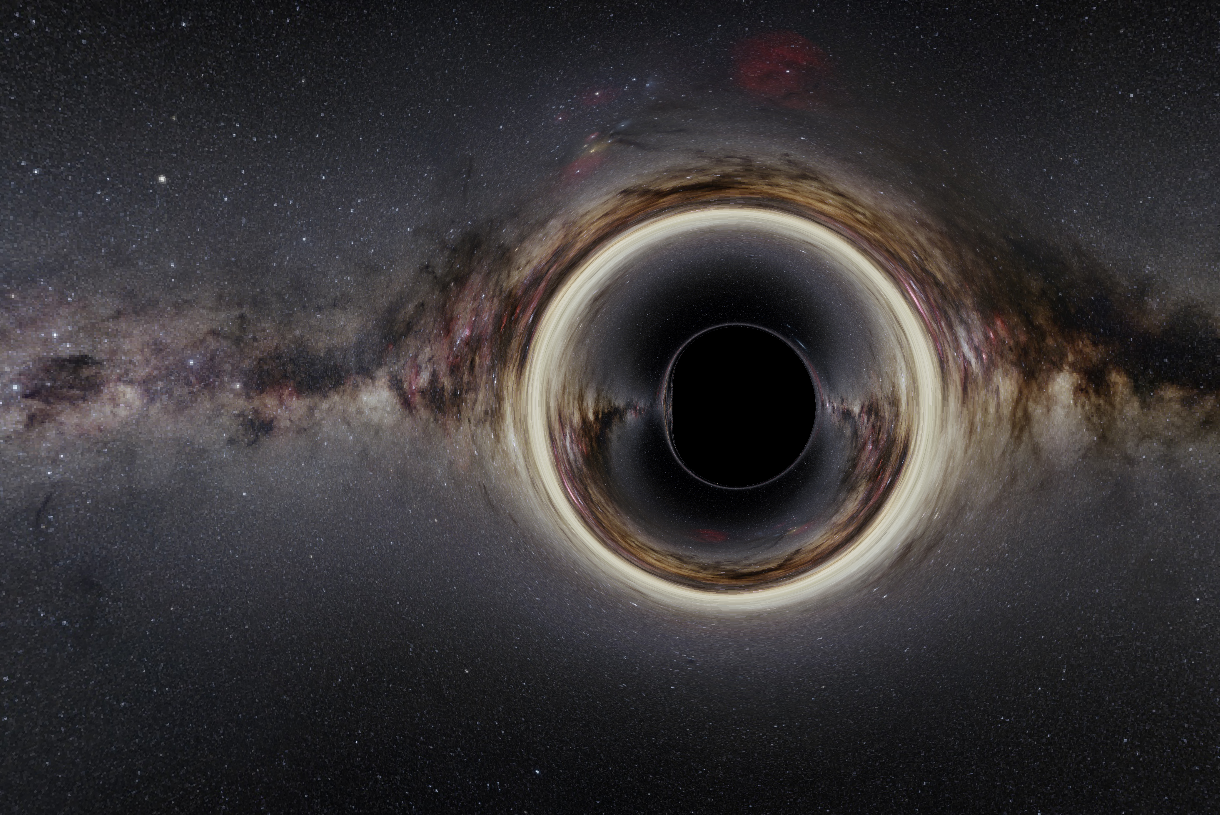
\includegraphics[width=\linewidth]{gfx/bh_texture_nodisk}
	\caption[Textured image without accretion disk]{Textured image without accretion disk}
	\label{fig:blackholenodisk}
\end{figure}

\autoref{fig:blackhole} is one example of a fully featured image with a cinematographic look: the celestial sphere is textured with an image of the Milky Way; an accretion disk around the black hole is added and a texture on the disk is rendered.

\autoref{fig:blackholenodisk} shows the same previous image, but rendered without the disk to better see the distortion produced by the black hole.

Furthermore, the rendered images can be plotted as three dimensional projections, letting the user observe the paths followed by the geodesics in order to understand how they were curved.

An example of this feature can be seen on \autoref{fig:3dprojection}, where four snapshots of the three dimensional projection are shown. Blue lines represent geodesics that come from the celestial sphere, red lines are geodesics that never existed, as they would have originated inside the black hole's horizon; finally, the green lines are the geodesics whose origin is on the accretion disk.

The computed information can rendered independently as a three dimensional projection or as an image. \autoref{fig:3dprojectionimage} shows the photography whose three dimensional representation was depicted on \autoref{fig:3dprojection}. In this case, the disk is textured with a coloured patched texture.

\begin{figure}[bth]
	\myfloatalign
	\subfloat[Top view.]
	{\frame{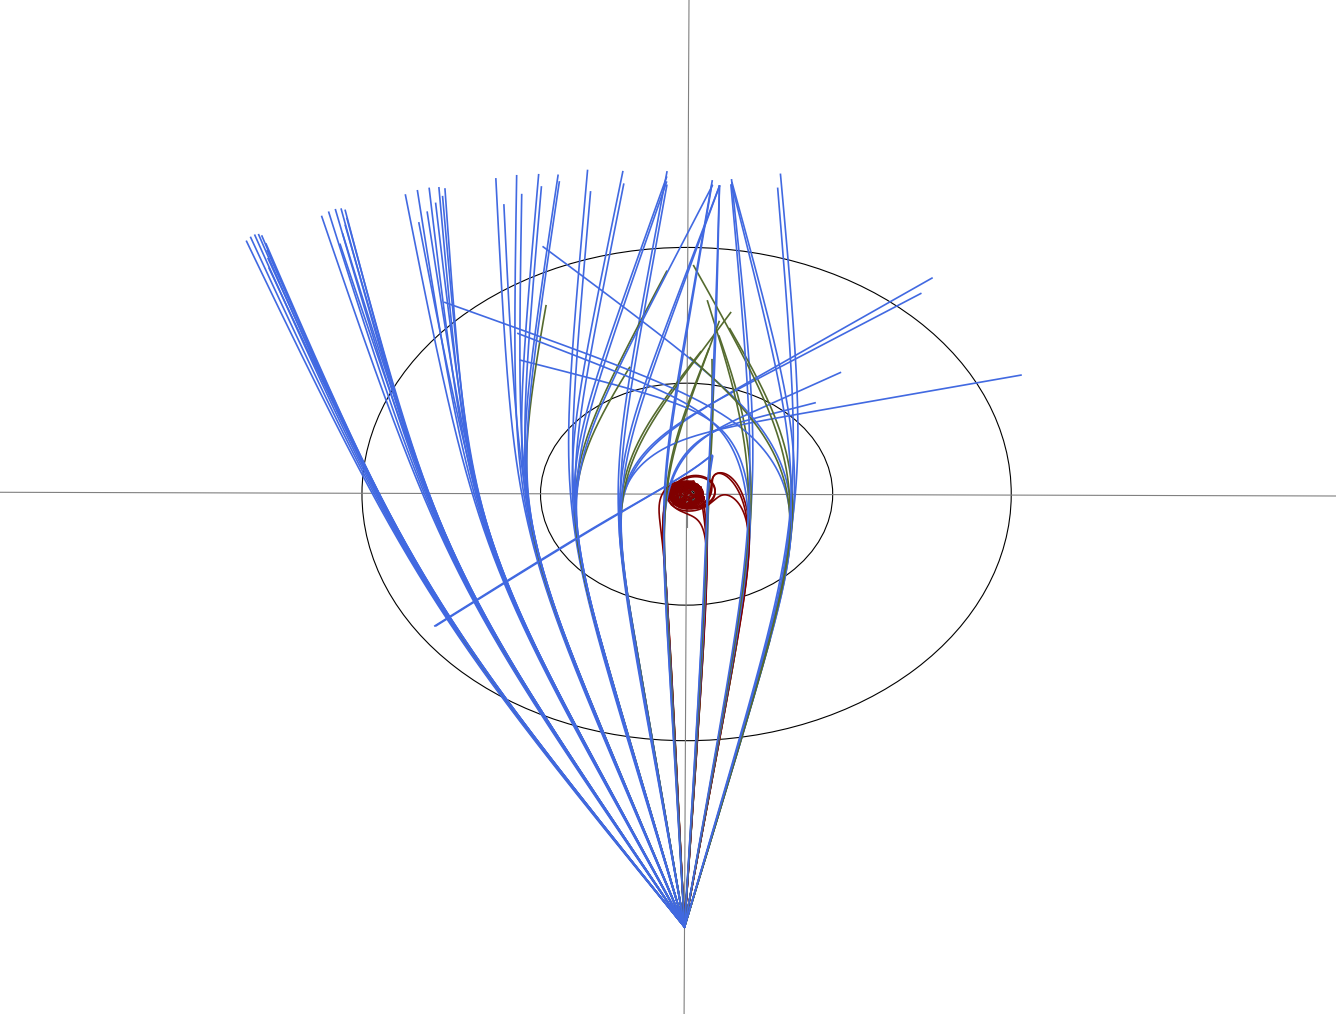
\includegraphics[width=.45\linewidth]{gfx/3d_01_top}}} \quad
	\subfloat[Right view.]
	{\frame{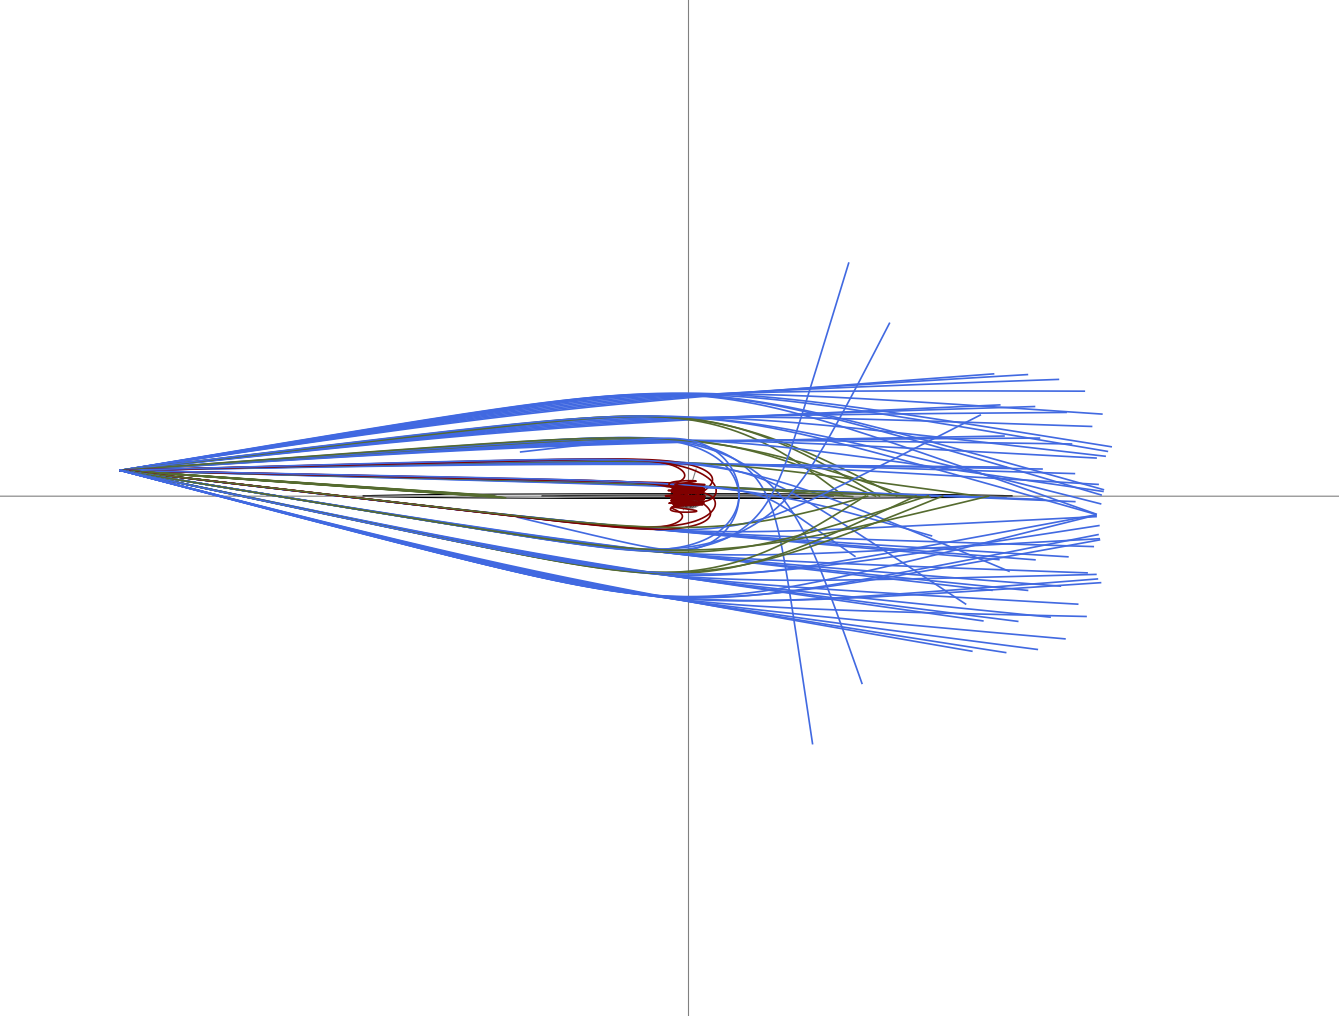
\includegraphics[width=.45\linewidth]{gfx/3d_01_right}}} \\
	\subfloat[Perspective view from behind.]
	{\frame{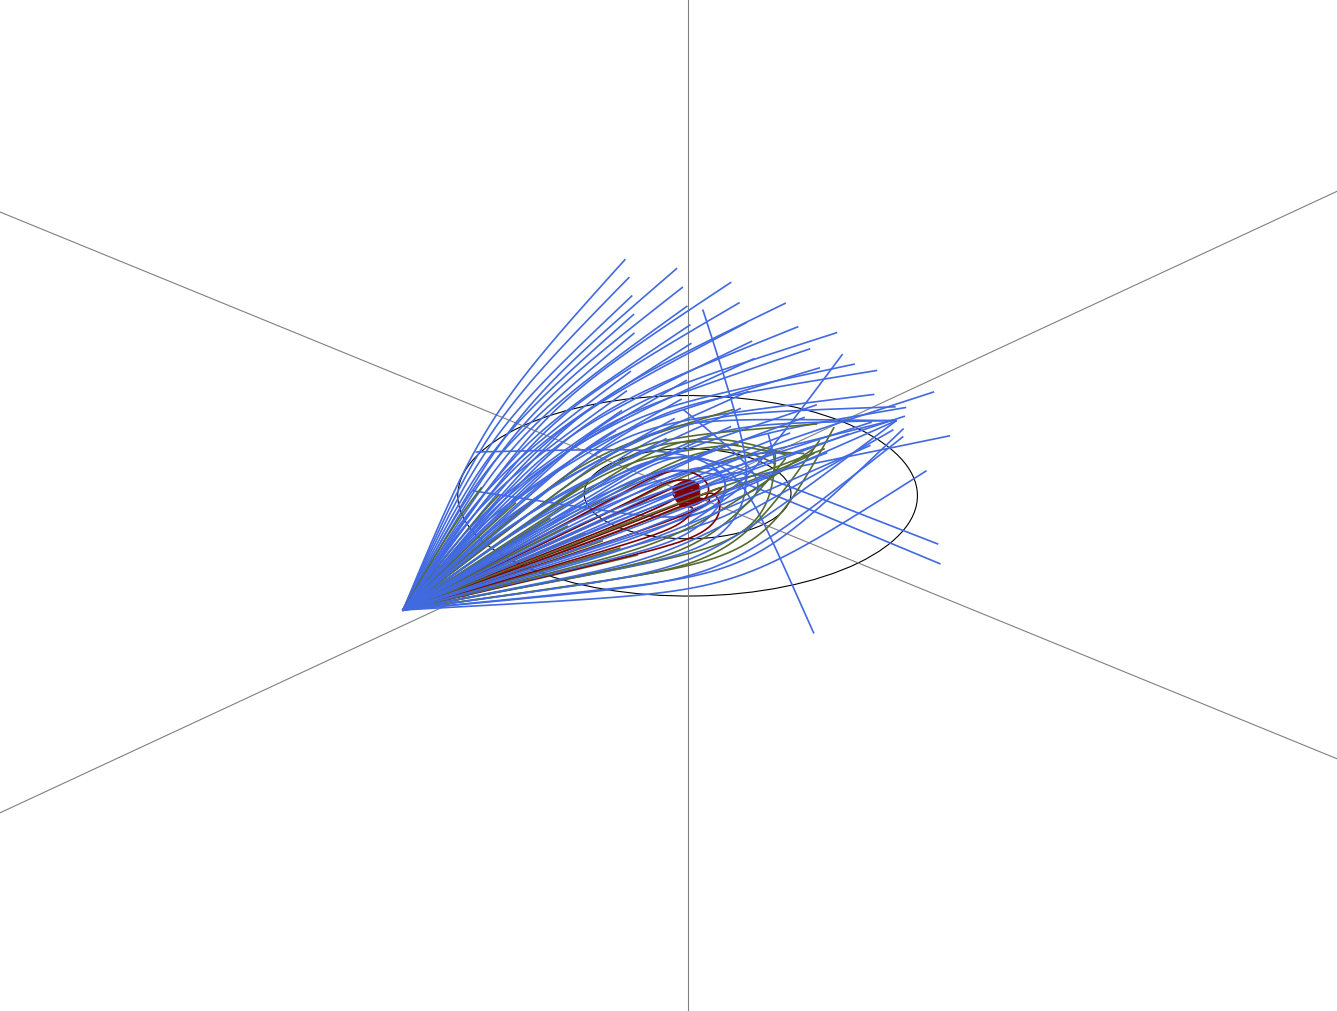
\includegraphics[width=.45\linewidth]{gfx/3d_01_perspective1}}} \quad
	\subfloat[Perspective view from the front side.]
	{\frame{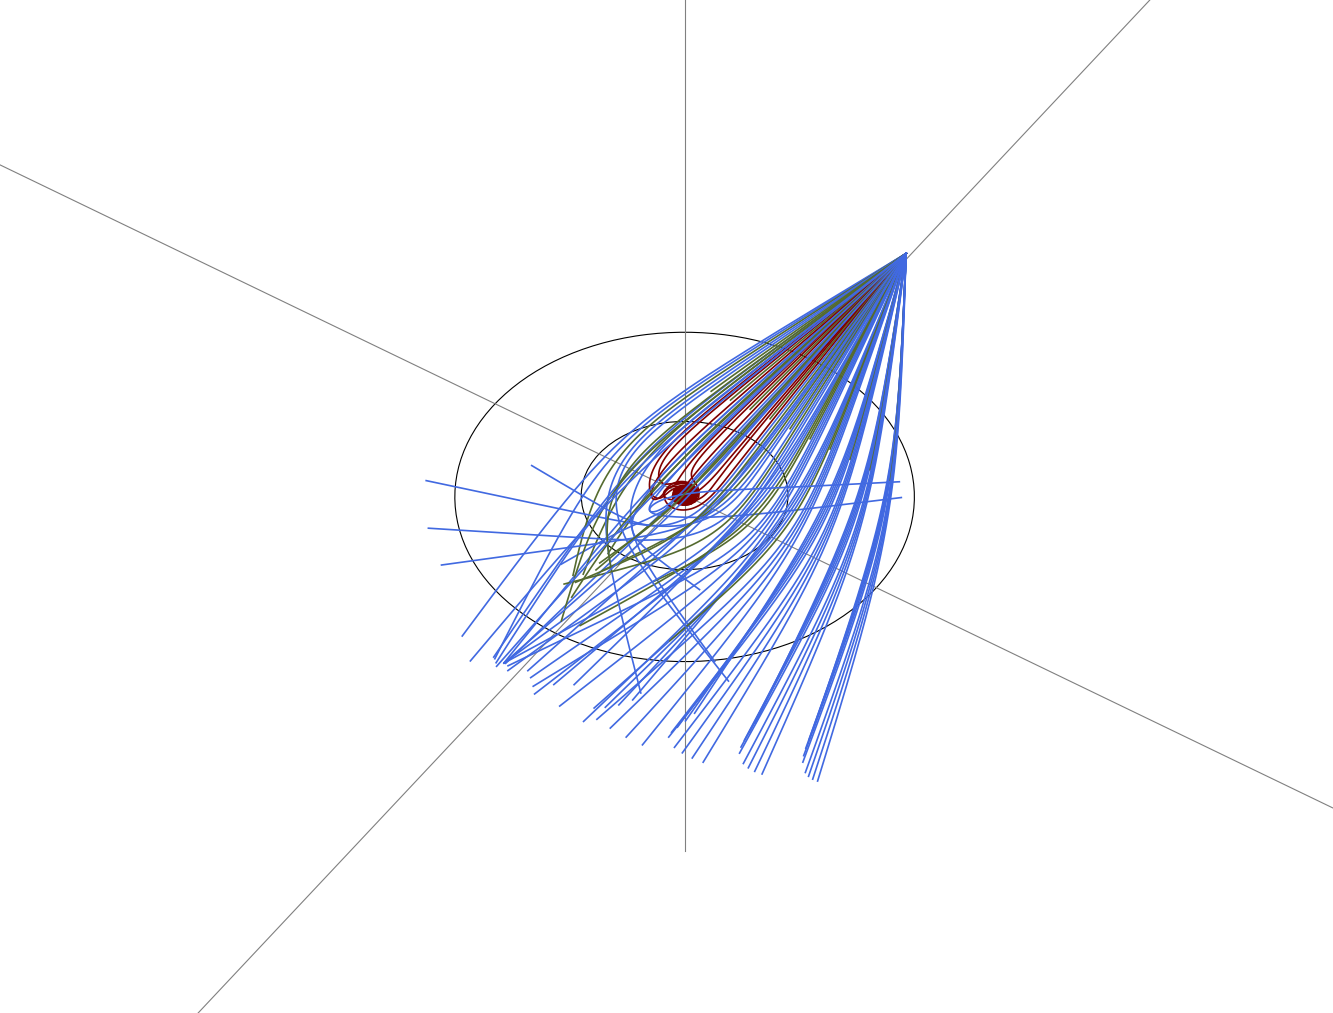
\includegraphics[width=.45\linewidth]{gfx/3d_01_perspective2}}}
	\caption[3D representation of the geodesics]{3D representation of the geodesics.}\label{fig:3dprojection}
\end{figure}

\begin{figure}[bth]
	\myfloatalign
	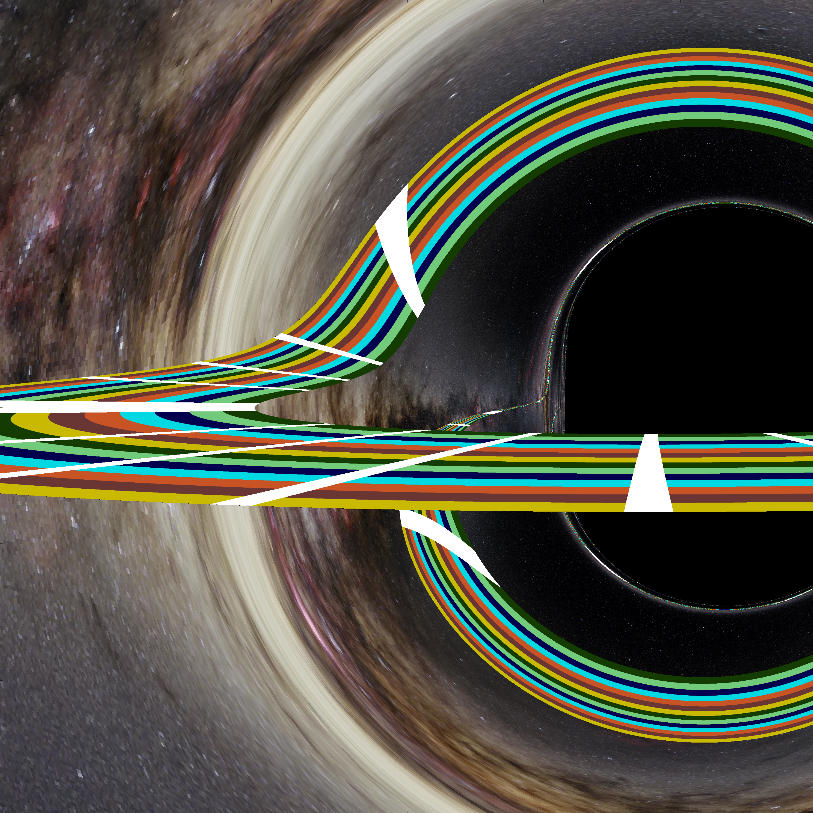
\includegraphics[width=.7\linewidth]{gfx/3d_01_image}
	\caption[Photography from a 3D scenario]{Photography of the 3D scenario rendered in \autoref{fig:3dprojection}}
	\label{fig:3dprojectionimage}
\end{figure}

\subsection{Computational Results}

This section covers the computational results of the implemented code; \ie, it studies the accuracy and efficiency of the ray tracer.

\subsubsection*{Runge-Kutta Solver Accuracy}

The \ac{RK} solver has been tested not only against the geodesics \ac{ODE} system, but against usual functions whose analytic expression is known. This basic test was done with two purposes:
\begin{enumerate}
	\item To test that the solver was accurate.
	\item To study the behaviour of the automatic step size computation.
\end{enumerate}

One example of this test can be seen on \autoref{fig:stepsize}, that shows the behaviour of the \ac{RK} solver on the Airy function $Bi(x)$. The orange line is its analytic expression, which is
\[
Bi(x) = \frac{1}{\pi} \int_0^\infty \cos\left(\frac{t^3}{3} + xt\right)dt,
\]
while the blue points are the solution computed by the \ac{RK} solver of the \ac{ODE} whose solution is $Bi(x)$, that is
\[
\frac{d^2y}{dx^2} - xy = 0.
\]

\begin{figure}[bth]
	\myfloatalign
	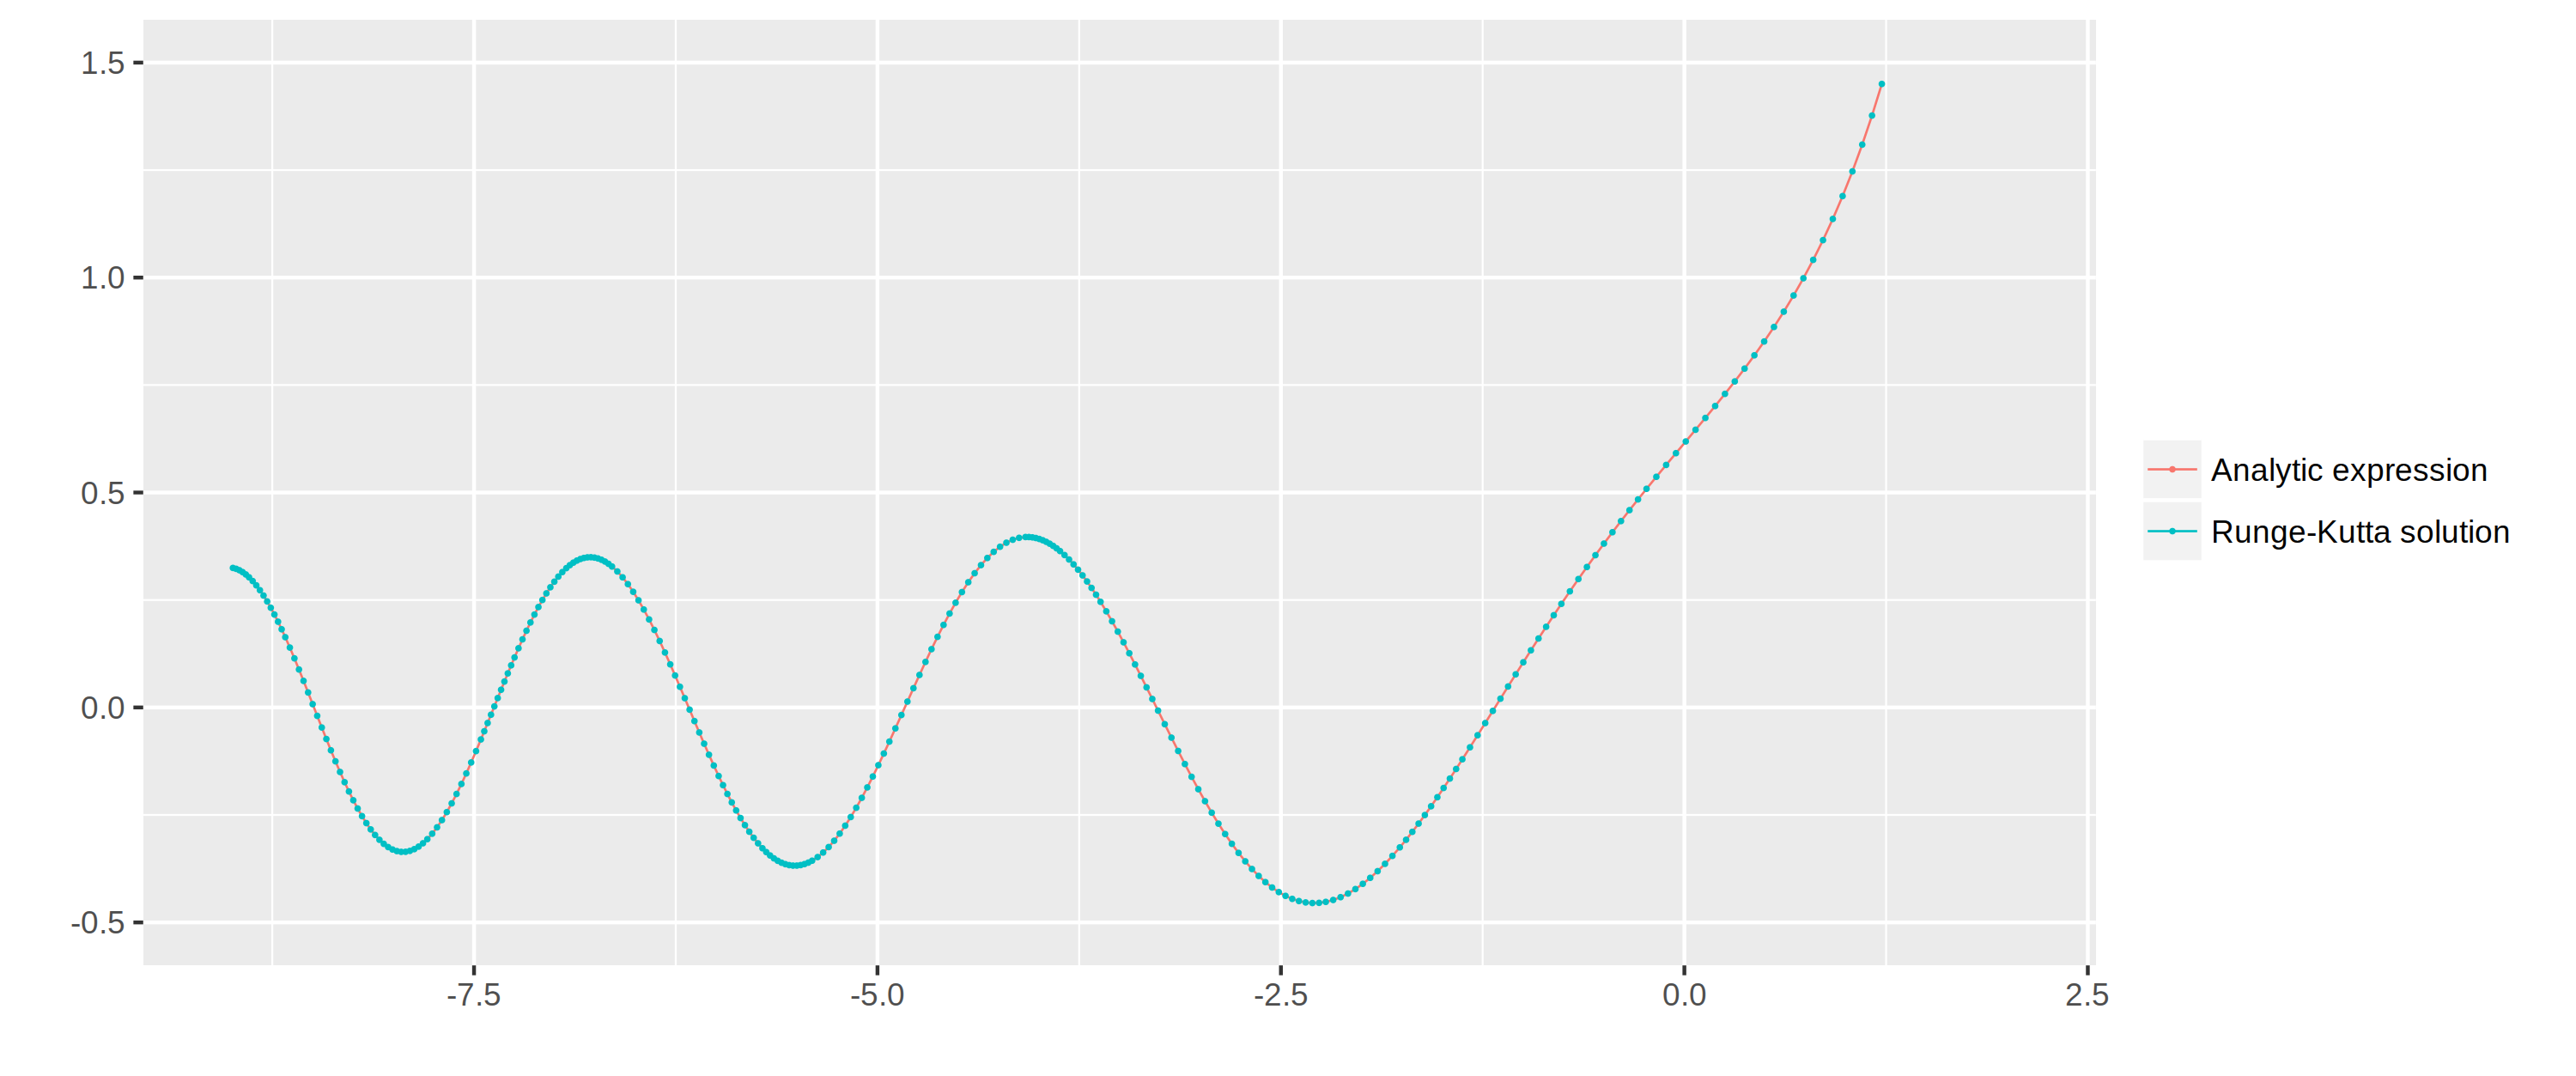
\includegraphics[width=1.3\linewidth]{gfx/analytic}
	\caption[Solver in an analytic function]{\ac{RK} solver in an analytic function}
	\label{fig:stepsize}
\end{figure}

It can be seen how the automatic step computation algorithm works smoothly: when the function can be approximated as a straight line, the step, which is the space between successive points, is very large. However, in intervals where the function changes rapidly its curvature, the algorithm reduces the step in order to better approximate the function value.

\begin{figure}[bth]
	\myfloatalign
	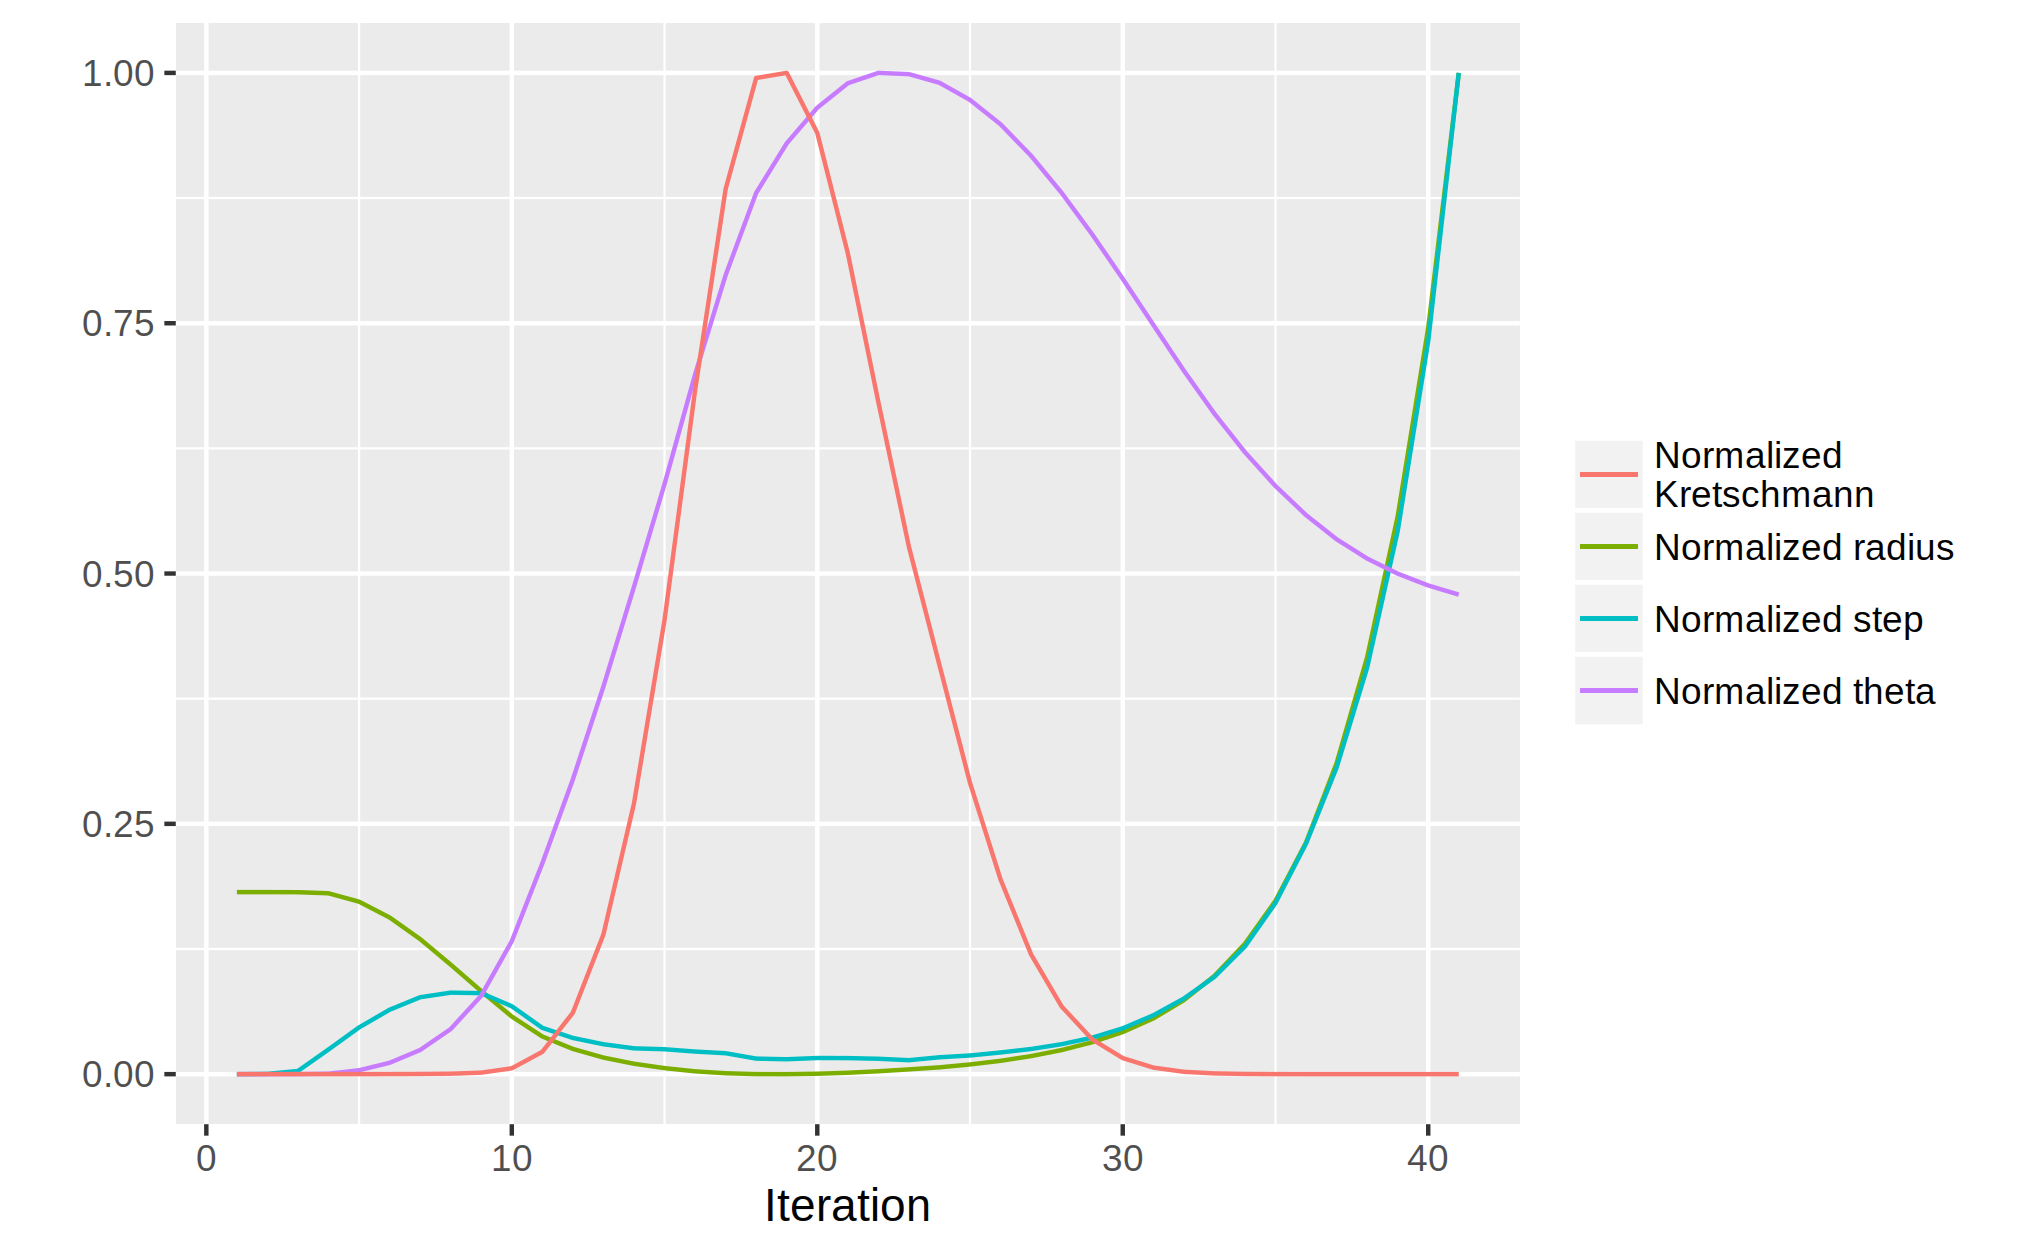
\includegraphics[width=1.2\linewidth]{gfx/kretschmann}
	\caption[Step, $r$, $\vartheta$ and Kretschmann]{Step, radius, $\vartheta$ and Kretschmann}
	\label{fig:kretschmann}
\end{figure}

This behaviour can also be seen on the geodesics \ac{ODE} system. \autoref{fig:kretschmann} shows the normalized values of four quantities:
\begin{enumerate}
	\item The Kretschmann invariant, which measures the curvature of the spacetime, and which is known to diverge in the singularity.
	\item The distance to the black hole.
	\item The value of the $\vartheta$ angle.
	\item The step computed by the automatic step algorithm.
\end{enumerate}

When the lightlike particle approaches the black hole; \ie, when the distance to the black hole decreases and, as a consequence, the Kretschmann increases, the system becomes unstable, and so the algorithm reduces the step size in order to better approximate its value.

In fact, both the step line and the radius line are very similar, showing the correlation between the computed step and the distance to the black hole centre.

\subsubsection*{Efficiency}

Regarding the efficiency of the ray tracer, a benchmark against a \ac{CPU} implementation has been done.

The \ac{CPU} implementation has essentially the same code that the \ac{GPU}-parallelized version, except for the obvious changes that were made to adapt the code to the \ac{CUDA} grid.

\autoref{fig:speedup} shows two benchmarks using both versions of the ray tracer: one with a Kerr spacetime where the black hole has a spin of $a = 0.0001$ and another one where the spin is $a = 0.999$.

For both benchmarks, the speed up is plotted, \ie, the line represented for each of them shows how many times faster is the \ac{GPU}-parallelized version against the \ac{CPU} implementation.

\begin{figure}[bth]
	\myfloatalign
	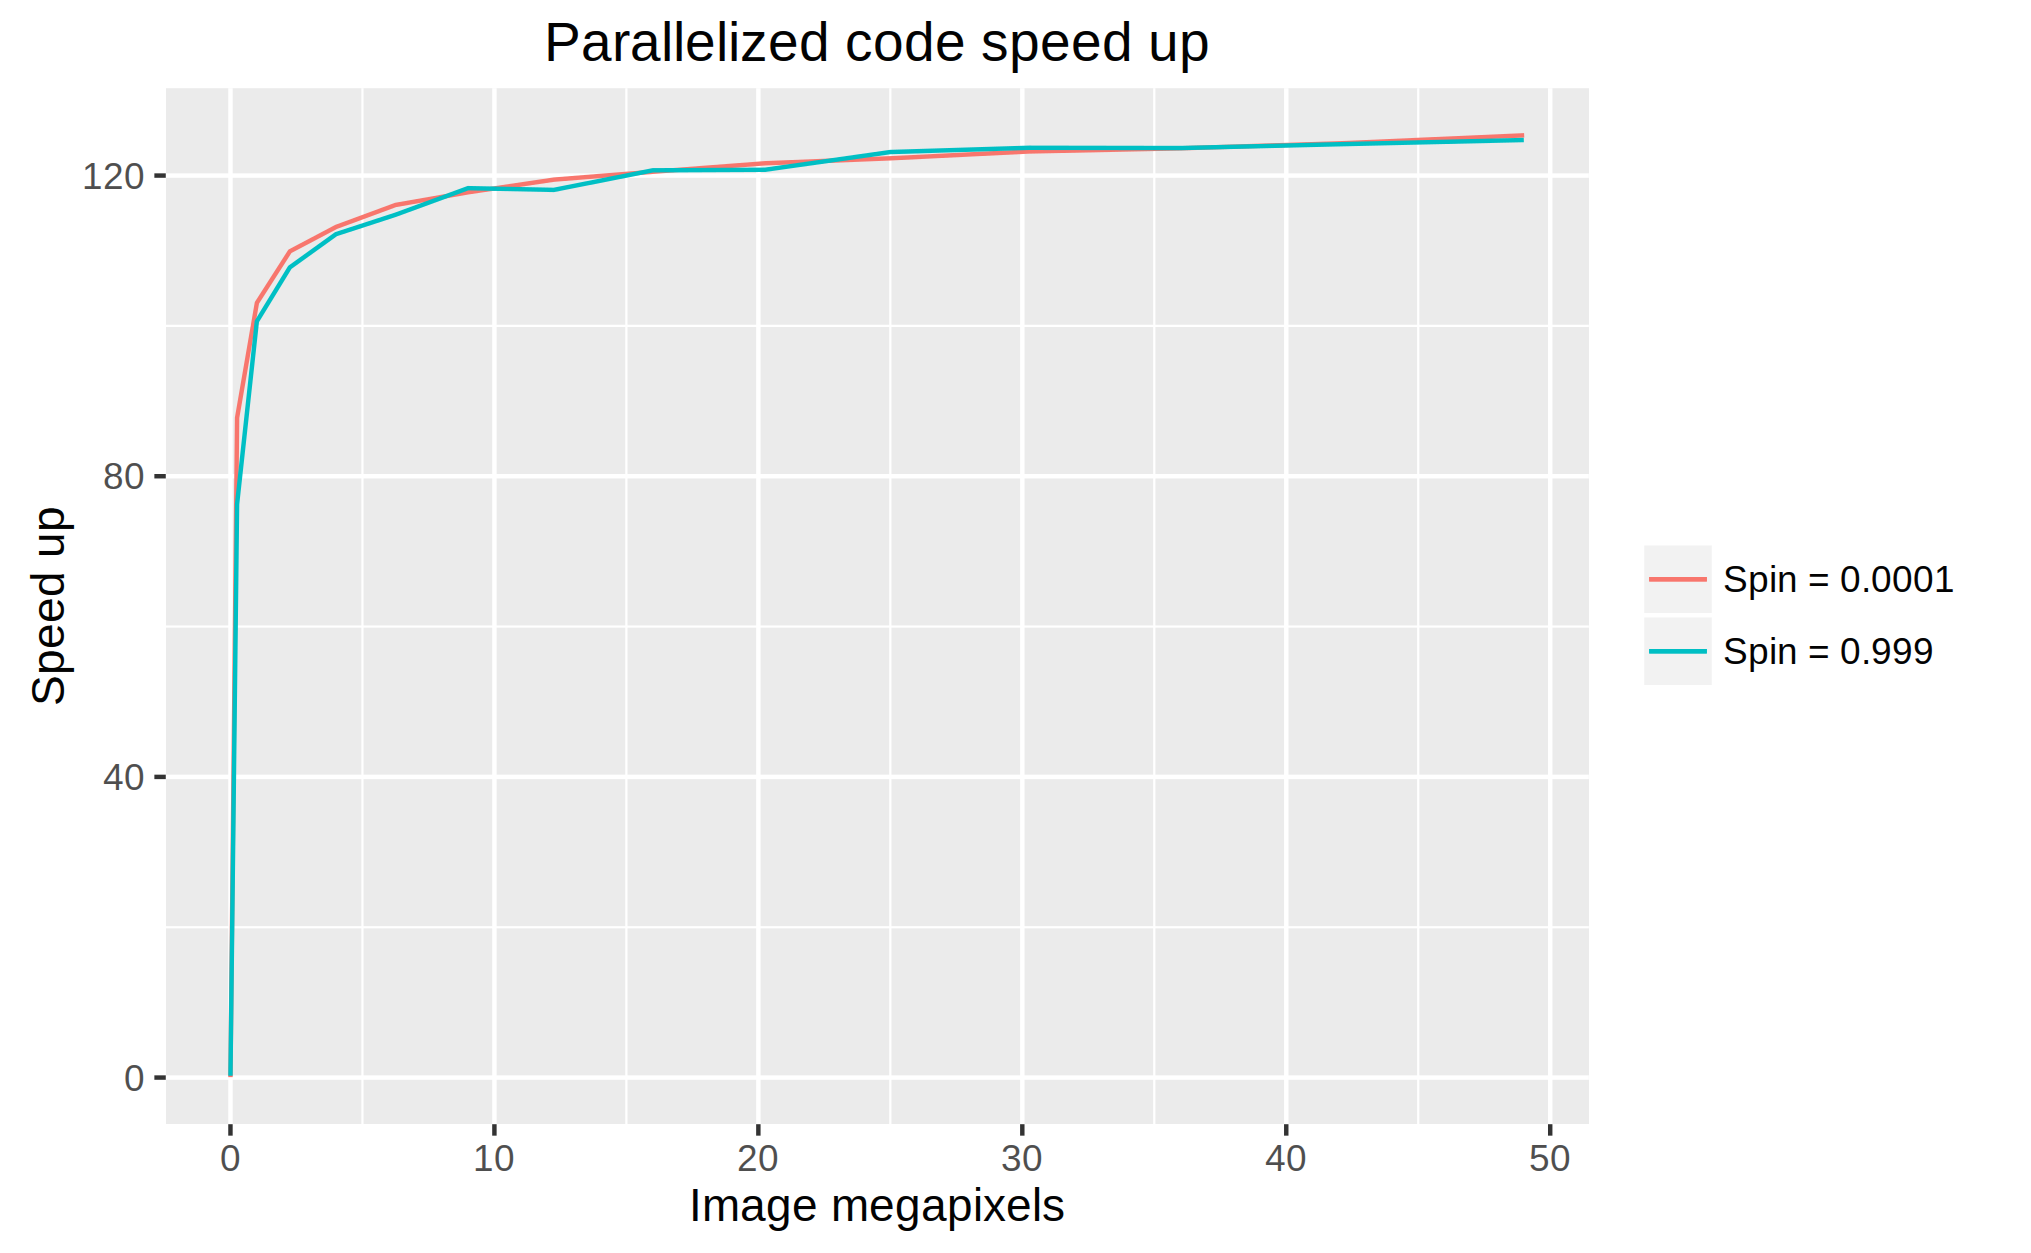
\includegraphics[width=1.2\linewidth]{gfx/speedup}
	\caption[Speed up with different spins]{Speed up with different spins}
	\label{fig:speedup}
\end{figure}

The speed up increases at a great speed when the number of pixels are augmented. It stabilizes around 20 megapixels with a speed up of about $125$. The mean speed up equals $108.5$ on the low spin case, whereas in the high spin case equals $107.2$. The maximum speedup obtained equals $125.3$ on the first case, with a maximum speed up of $124.7$ on the second.

As we can see, these numbers do not vary too much depending on the spin, so the speed up seems to be stable against these changes. This figure summarises the power of the \ac{GPGPU}, that can increase the performance of a piece of software by several orders of magnitude.


\subsection{Scientific Results}

The main objective of the ray tracer implementation was to serve as a tool for scientists to study properties of the Kerr spacetime. This section summarises some of these interesting features.

\subsubsection*{Spin}

The effect of the black hole spin on its surroundings has been studied in two ways.

First of all, we have generated images without any accretion disk and without textures for the celestial sphere. This gives us binaries images where the black pixels represent the shadow of the black hole and the white pixels the geodesics that came from the celestial sphere.

\autoref{fig:shadow} shows four images taken with the same camera, which is placed on the equatorial plane, with a null speed and focusing the black hole's centre. The only change between images is the black hole's spin.

The first one shows a perfect sphere. This is the edge case where the Kerr metric can be reduced to the more simple Schwarzschild metric.

\autoref{fig:shadow-b} and \autoref{fig:shadow-c} shows the same image with an increased spin. There is a slight change on the virtual position of the shadow and, although it is difficult to see, the shape is not circular.

The edge case, depicted on \autoref{fig:shadow-d}, makes clear the effect of a large spin on the shadow of the black hole. As it curves the geodesics rapidly, it is seen slightly moved to the right and with a flat side on the left: if the spin were of this same magnitude but negative, the image would be vertically mirrored.

\begin{figure}[bth]
	\myfloatalign
	\subfloat[Spin $\approx$ 0]
	{\frame{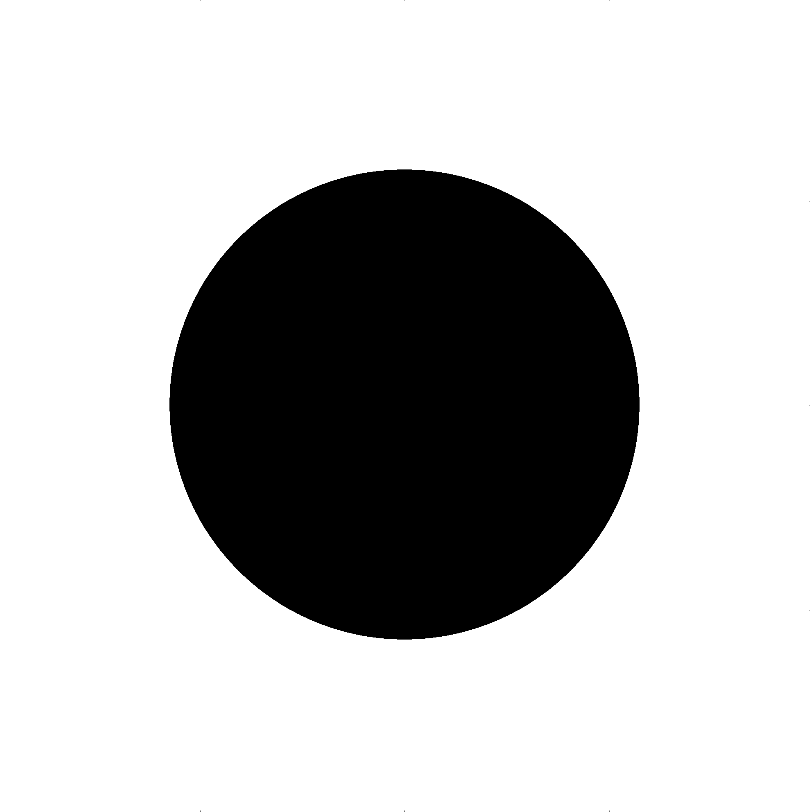
\includegraphics[width=.35\linewidth]{gfx/bh_shadow_spin0001}}} \quad
	\subfloat[Spin = 0.25]
	{\label{fig:shadow-b}%
		\frame{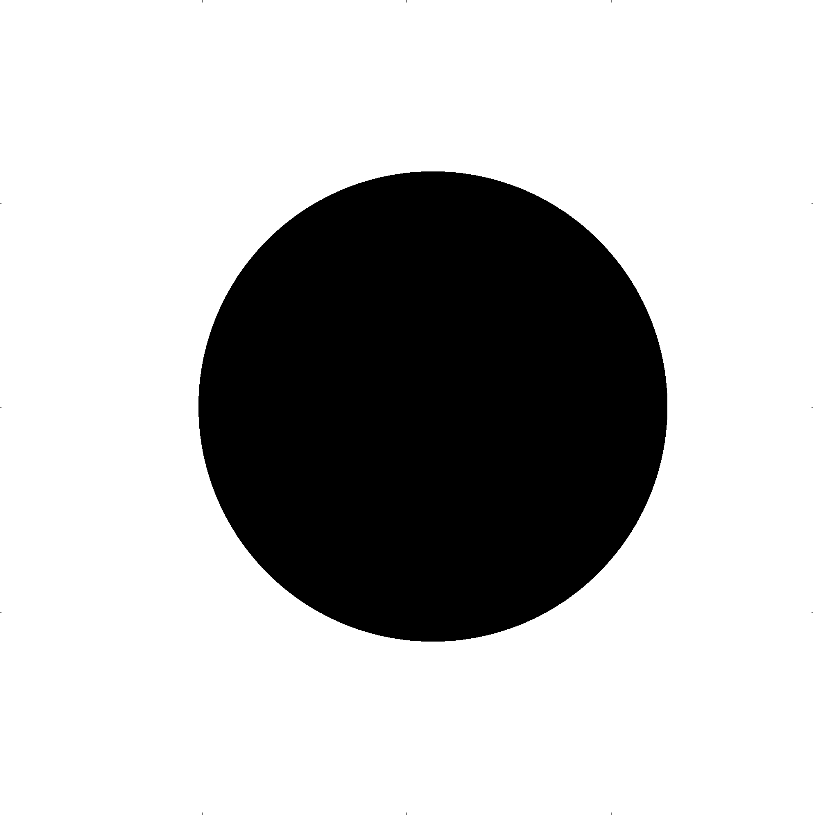
\includegraphics[width=.35\linewidth]{gfx/bh_shadow_spin25}}} \\
	\subfloat[Spin = 0.75]
	{\label{fig:shadow-c}%
		\frame{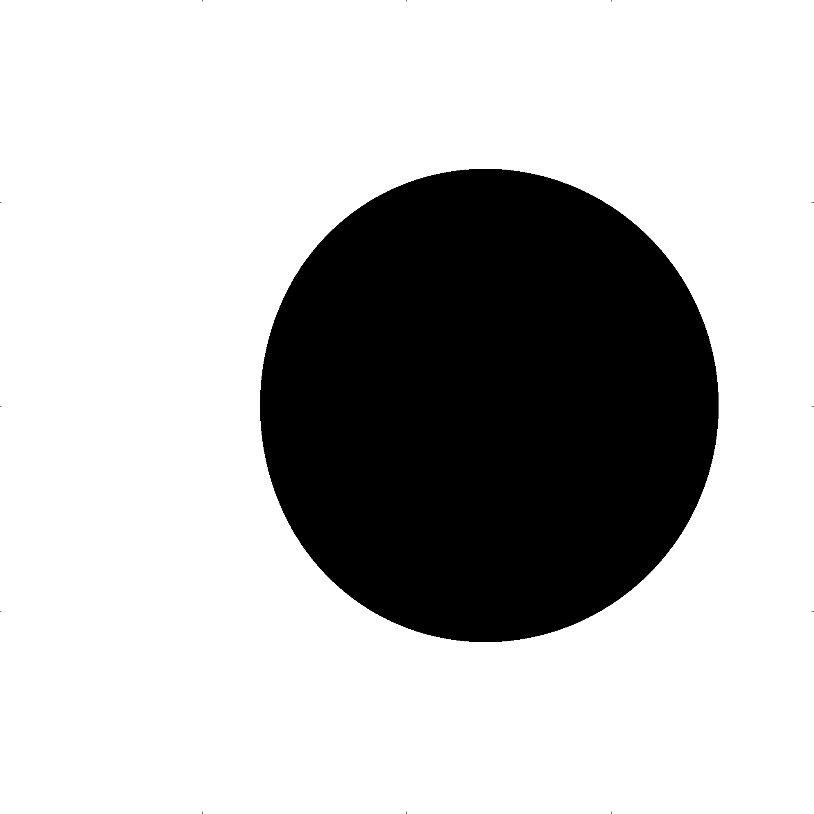
\includegraphics[width=.35\linewidth]{gfx/bh_shadow_spin75}}} \quad
	\subfloat[Spin $\approx$ 1]
	{\label{fig:shadow-d}%
		\frame{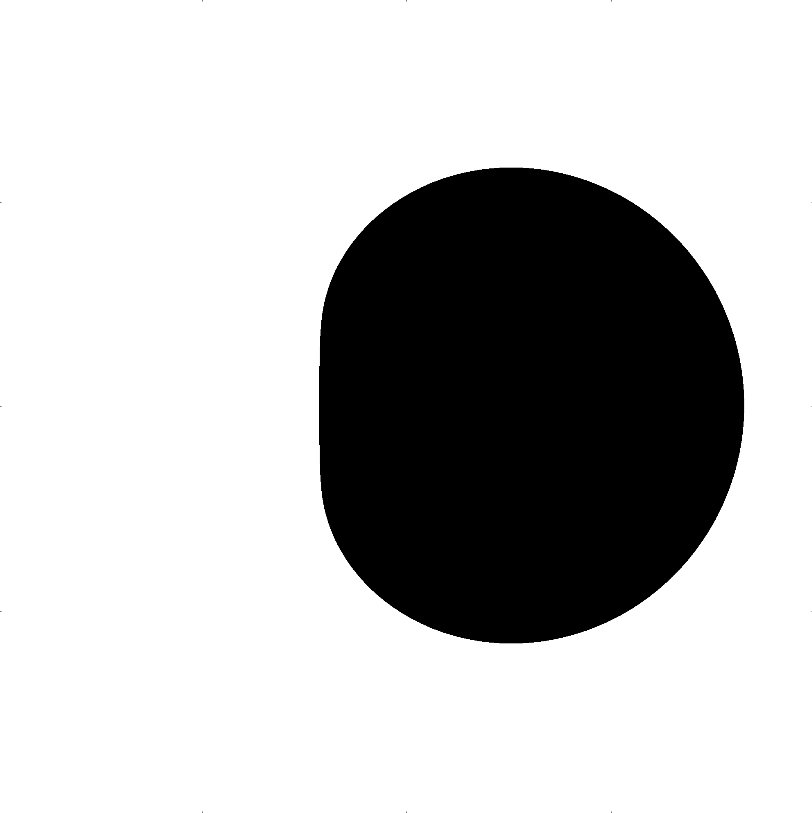
\includegraphics[width=.35\linewidth]{gfx/bh_shadow_spin999}}}
	\caption[Black hole shadow for different spins]{Black hole shadow for different spins}\label{fig:shadow}
\end{figure}

It is also interesting to see what happens with straight lines that fall inside the black hole.

Imagine an accretion disk around the black hole, with its inner radius minor than the horizon radius and an infinite outer radius. If we visualize this disk with a patched texture made by white and red squares, we can see the effect of the spin on its shape.

\autoref{fig:xmas-a} shows the most simple version of this scenario, where the black hole does not rotate: straight lines falling inside the black hole on the equatorial plane remain intact.

Taking this as the base case, we can see what happens when we increase the black hole's spin. \autoref{fig:xmas-b} and \autoref{fig:xmas-c} shows the scenario for spins of $0.25$ and $0.75$. The straight lines start to rotate accordingly with the black hole.

The most interesting image is depicted on \autoref{fig:xmas-d}, where we see an extreme spin of nearly 1. The lines curve greatly when they approach the shadow, and start rotating rapidly when they are close to the horizon.

\begin{figure}[bth]
	\myfloatalign
	\subfloat[Spin $\approx$ 0]
	{\label{fig:xmas-a}%
		\frame{
\includegraphics[width=.35\linewidth]{gfx/bh_xmas_spin0001}}} \quad
	\subfloat[Spin = 0.25]
	{\label{fig:xmas-b}%
		\frame{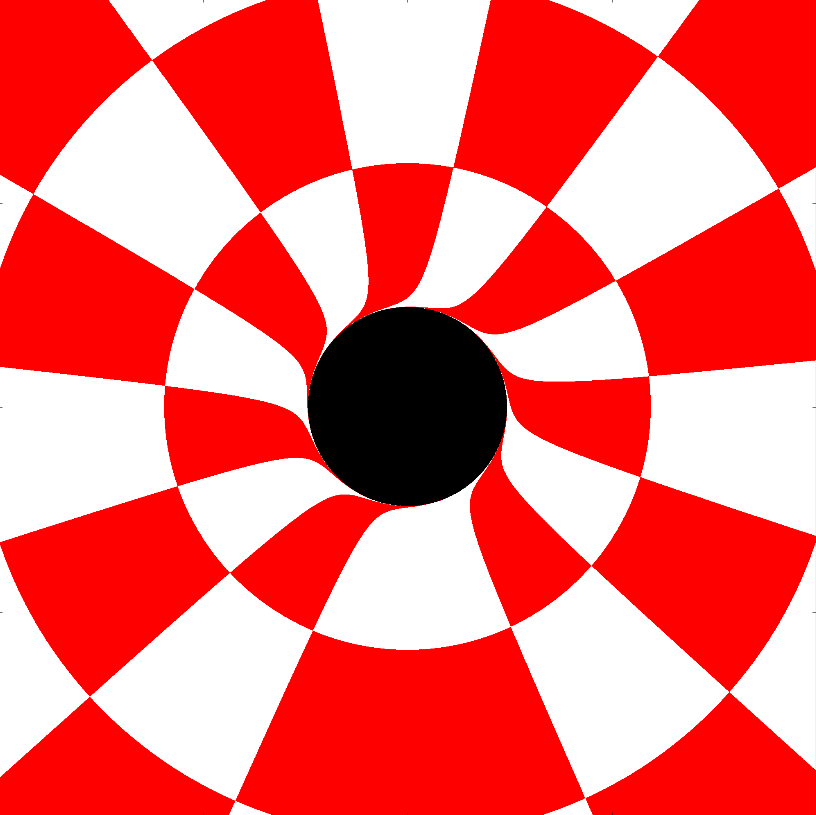
\includegraphics[width=.35\linewidth]{gfx/bh_xmas_spin25}}} \\
	\subfloat[Spin = 0.75]
	{\label{fig:xmas-c}%
		\frame{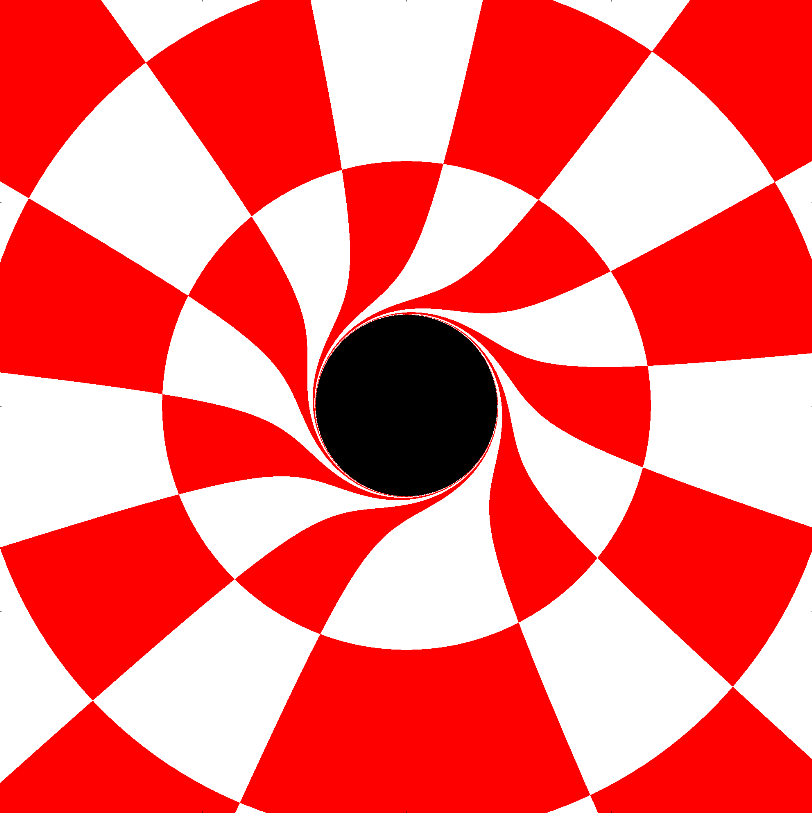
\includegraphics[width=.35\linewidth]{gfx/bh_xmas_spin75}}} \quad
	\subfloat[Spin $\approx$ 1]
	{\label{fig:xmas-d}%
		\frame{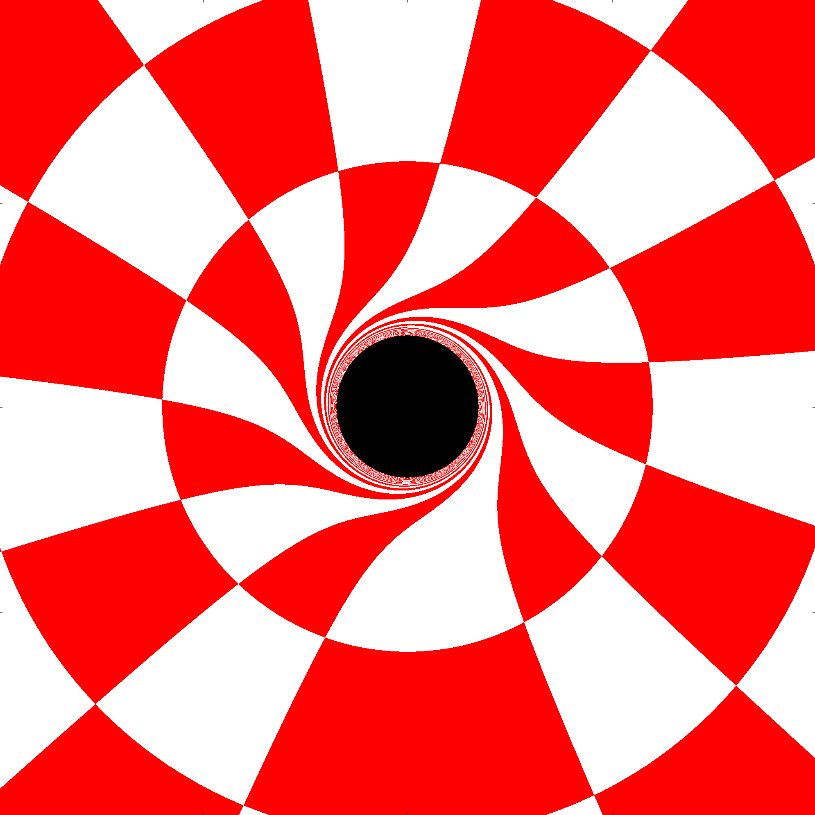
\includegraphics[width=.35\linewidth]{gfx/bh_xmas_spin999}}}
	\caption[Black hole shadow for different spins]{Black hole shadow for different spins}\label{fig:xmas}
\end{figure}

\subsubsection*{Shadow}

One can map a texture on the black hole's horizon to really know what we are seeing when looking at the shadow.

\autoref{fig:texhoriz} shows such an image, where a patched texture drawing the meridians and the parallels has been mapped onto the horizon's surface.

This image tells us that, when we are looking at the shadow of a Kerr black hole, we are seeing the whole surface of the horizon, not just the side facing to us.

\begin{figure}[bth]
	\myfloatalign
	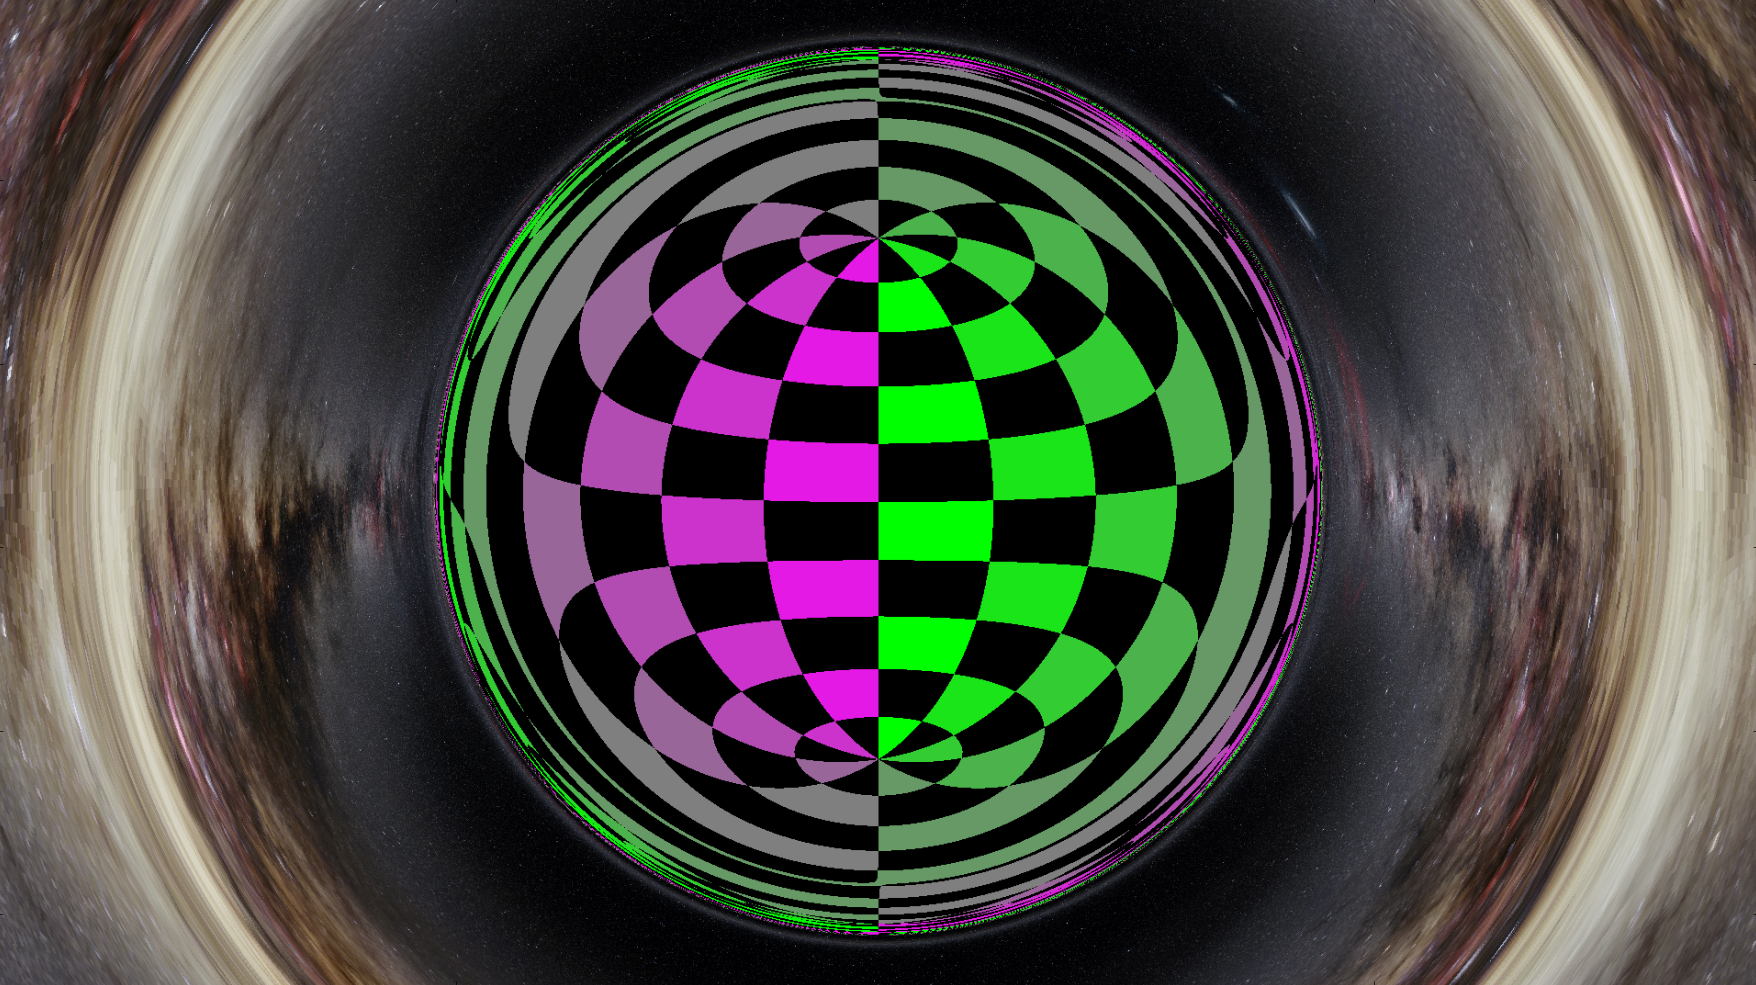
\includegraphics[width=.8\linewidth]{gfx/gridhorizon}
	\caption[Textured horizon]{Textured horizon.}
	\label{fig:texhoriz}
\end{figure}

\subsubsection*{Accretion Disk}

\begin{figure}[bth]
	\myfloatalign
	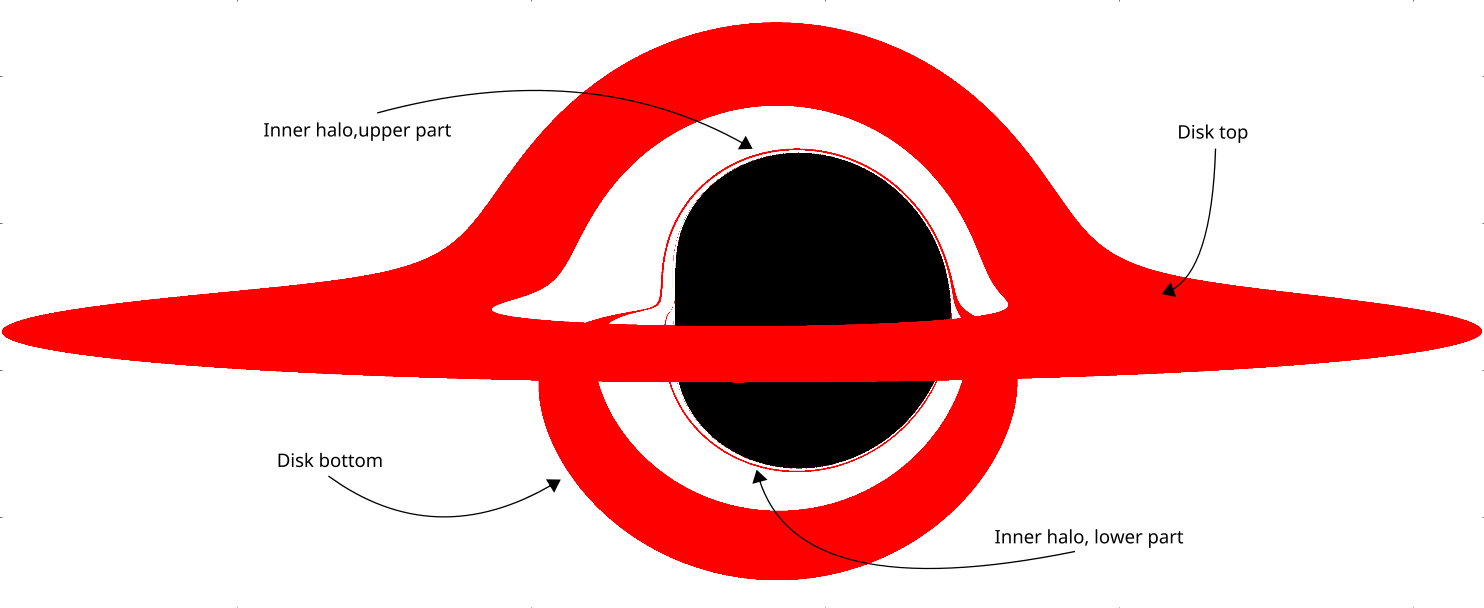
\includegraphics[width=\linewidth]{gfx/bh_simple}
	\caption[Accretion disk explained]{Accretion disk explained}
	\label{fig:explanation}
\end{figure}

The curvature of the disk around the black hole is really interesting. It let us understand the nature of the distortion produced by the spacetime.

Let us set up a simple image where the shadow is depicted with black pixels, the celestial sphere with white pixels and the disk with red ones.

\autoref{fig:explanation} shows this image, where we have noted the different parts of the disk we will talk about. The big stripe crossing the shadow that gets over it is the top of the disk. The lower stripe, that gets closer to the shadow and goes around on top of it is the disk bottom. We will denote the thin line just on top of the shadow as the upper part of the inner halo, where the thin line just below it will be called lower part of the inner halo.

It is interesting to visualize the geodesics that hit the disk in order to understand the processes that lead us to see the disk with such a great distortion.

First of all, we can describe the disk bottom: it is formed by lightlike particles that travel below the black hole and hit the disk just at the back of the shadow. A three dimensional projection of a set of these geodesics can be seen on \autoref{fig:under_disk}.

\begin{figure}[bth]
	\myfloatalign
	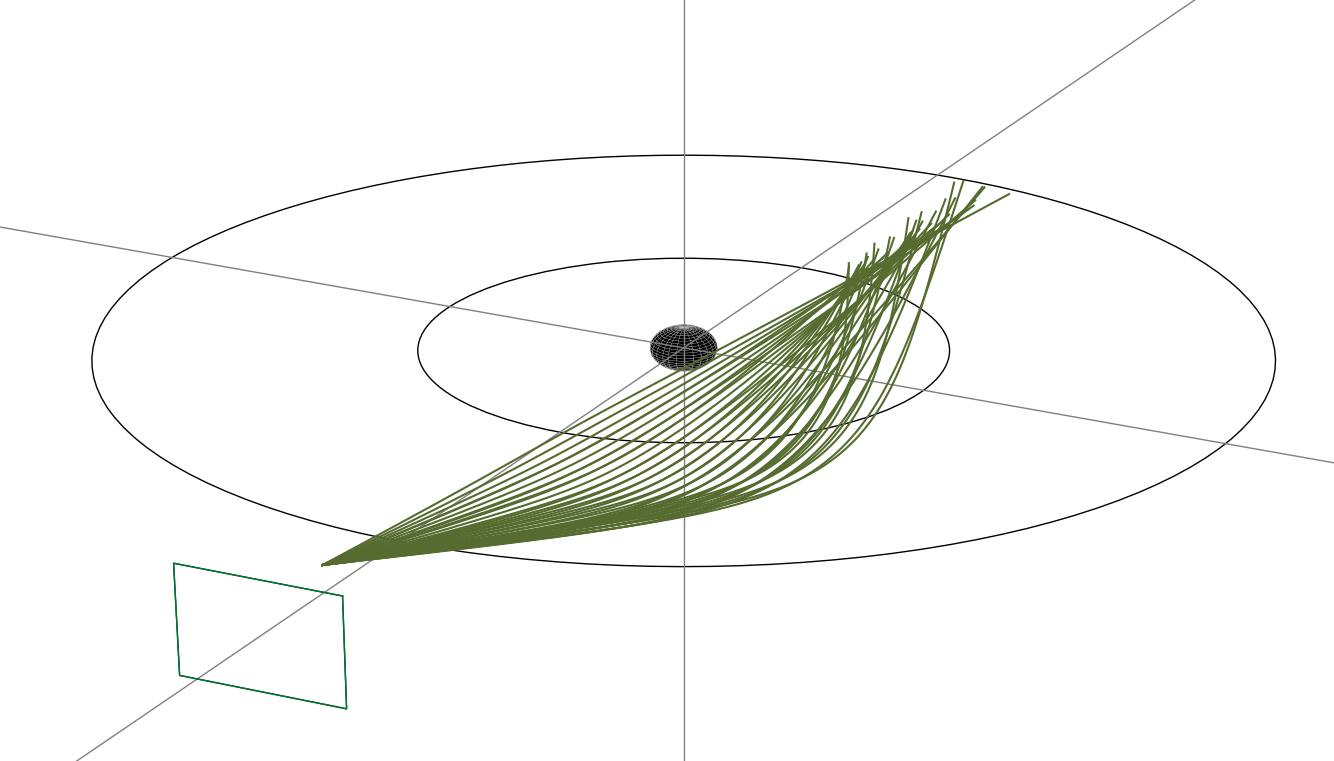
\includegraphics[width=.65\linewidth]{gfx/under_disk}
	\caption[Disk bottom]{Disk bottom.}
	\label{fig:under_disk}
\end{figure}

One of the most interesting parts of the disk distortion is the inner halo. \autoref{fig:insidehalo} shows a set of geodesics that formed its final image.

Furthermore, we can select the geodesics that form the upper part of the inner halo. \autoref{fig:upperhalo} shows the intricate paths followed by these geodesics, that twist around the black hole, get behind the disk and scatter to cover a great part of the bottom part of the disk.

\autoref{fig:wholehalo} summarises all this tour by plotting all geodesics that form the inner halo in just one image.

\begin{figure}[bth]
	\myfloatalign
	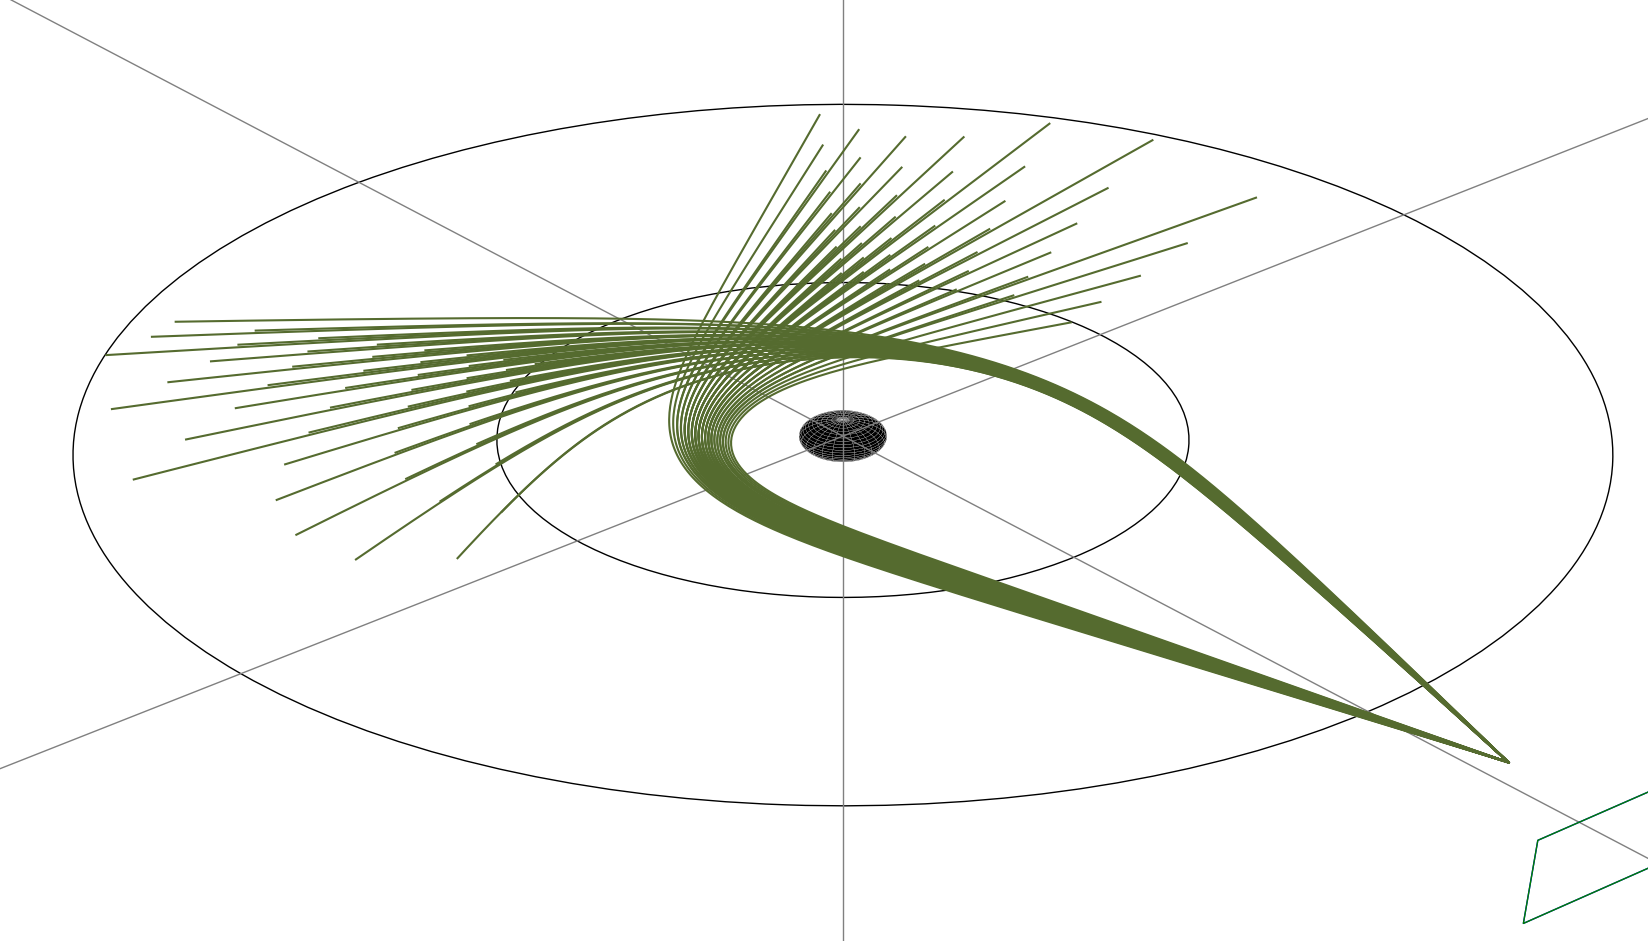
\includegraphics[width=.6\linewidth]{gfx/disk_inside_halo}
	\caption[Inner halo]{Inner halo.}
	\label{fig:insidehalo}
\end{figure}

\begin{figure}[bth]
	\myfloatalign
	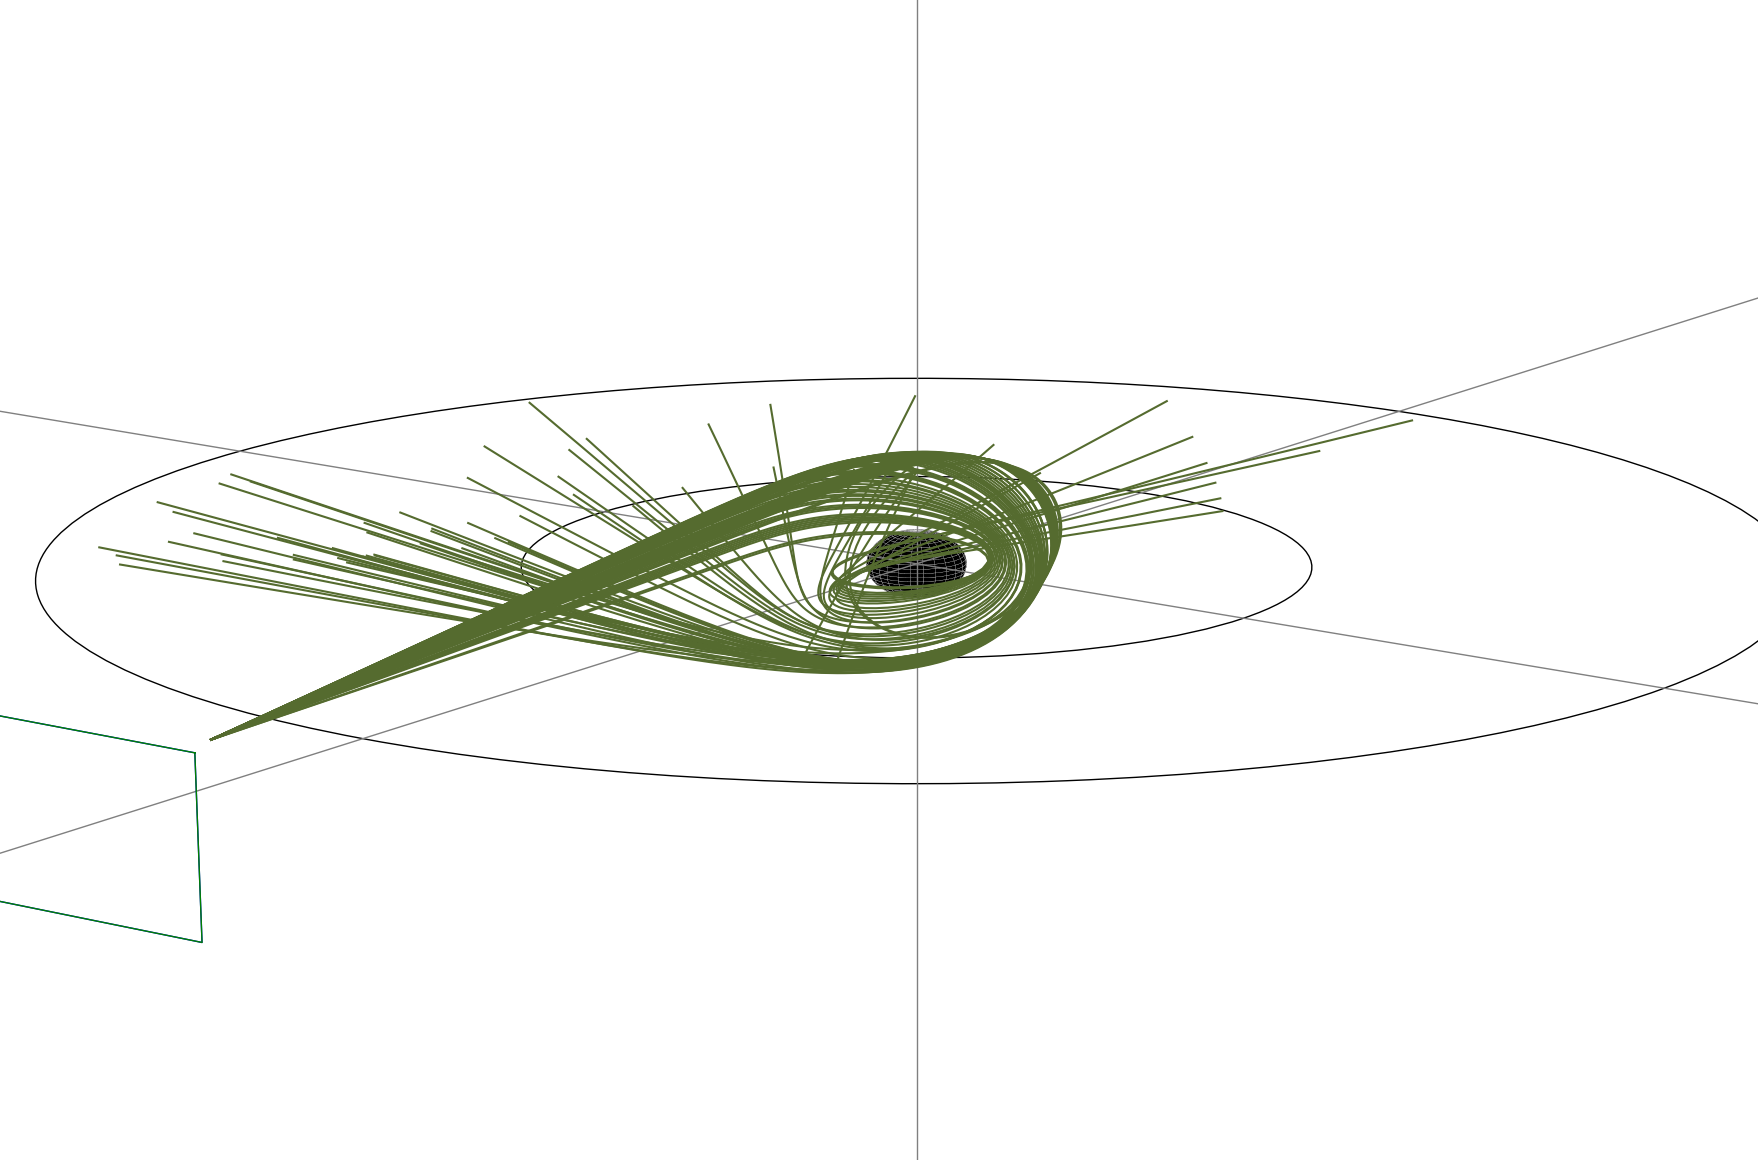
\includegraphics[width=.6\linewidth]{gfx/disk_inside_halo_superior}
	\caption[Upper part of the inner halo]{Upper part of the inner halo.}
	\label{fig:upperhalo}
\end{figure}

\begin{figure}[bth]
	\myfloatalign
	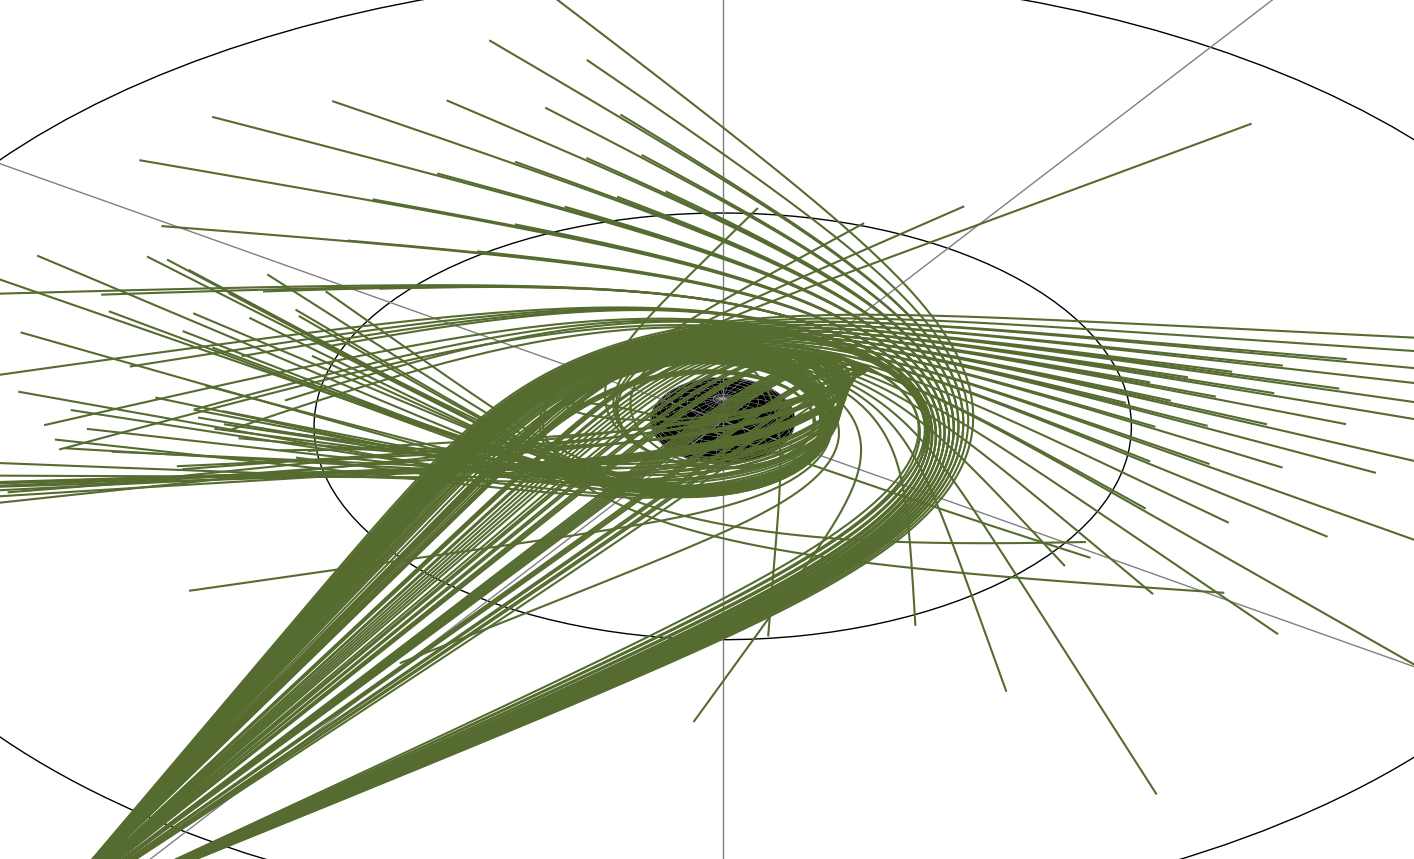
\includegraphics[width=.5\linewidth]{gfx/halo_entero}
	\caption[Geodesics forming the disk image]{Geodesics forming the disk image.}
	\label{fig:wholehalo}
\end{figure}

We can visualize, on the disk, the final point of the geodesic on the camera. In \autoref{fig:cathegories}, the black points represent the inner halo, the red points belong to the disk bottom, the green ones to the disk top and, finally, the blue points are the lower big stripe of the bottom disk.

\begin{figure}[bth]
	\myfloatalign
	{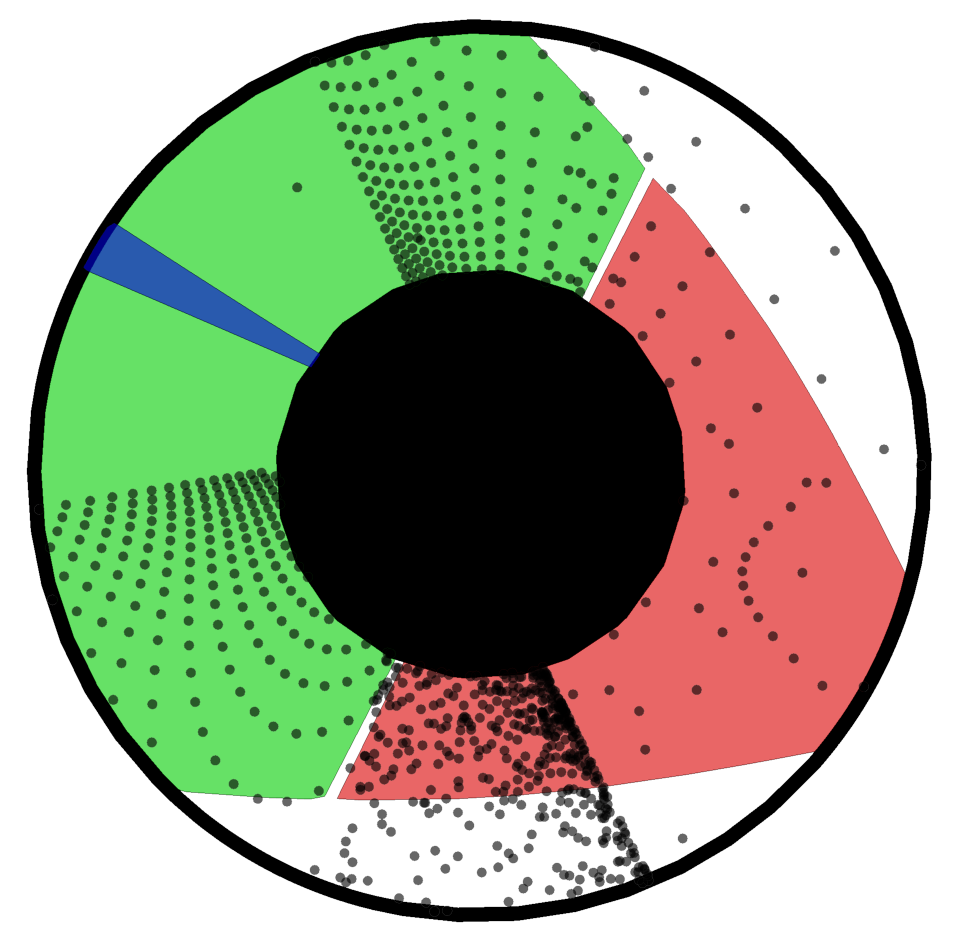
\includegraphics[width=.35\linewidth]{gfx/disk_cathegorization}} \quad
	{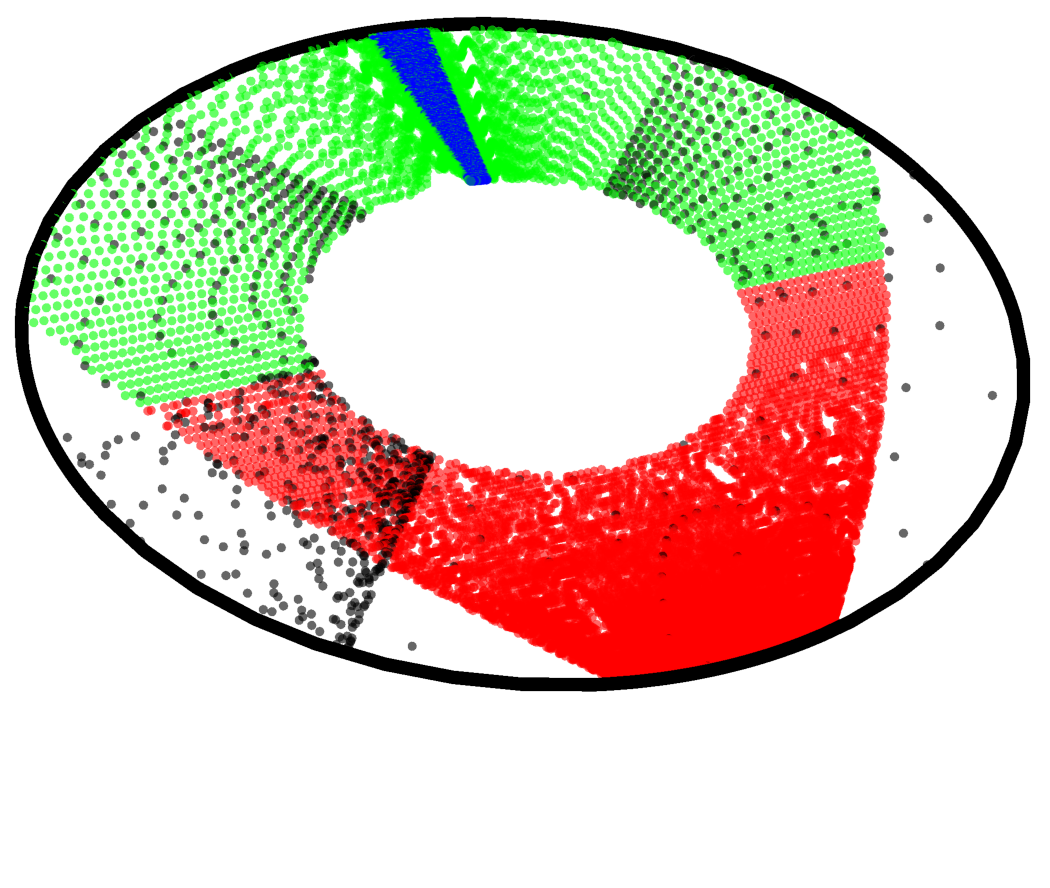
\includegraphics[width=.35\linewidth]{gfx/disk_cathegorization2}}
	\caption[Disk cathegorization]{Disk cathegorization.}
	\label{fig:cathegories}
\end{figure}

Finally, \autoref{fig:detail} shows a close up of the left side of the shadow where even more halos are appreciated. This time, for the sake of its beauty, a texture on the celestial sphere is added and the disk is drawn completely white.

\begin{figure}[bth]
	\myfloatalign
	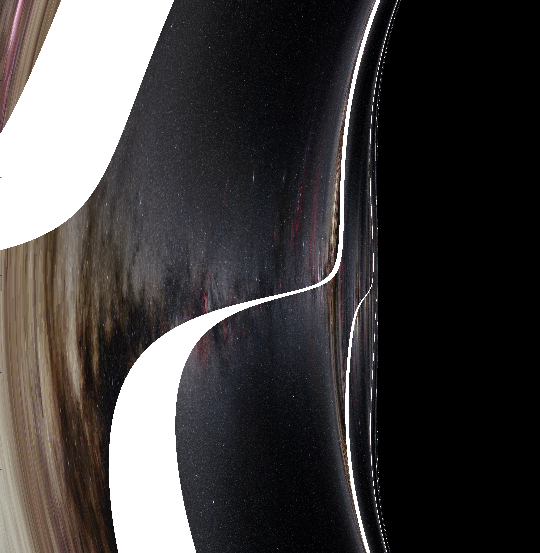
\includegraphics[width=.6\linewidth]{gfx/bh_detail_texture_disk-white}
	\caption[Close up of the shadow]{Close up of the shadow.}
	\label{fig:detail}
\end{figure}

\begin{figure}[bth]
	\myfloatalign
	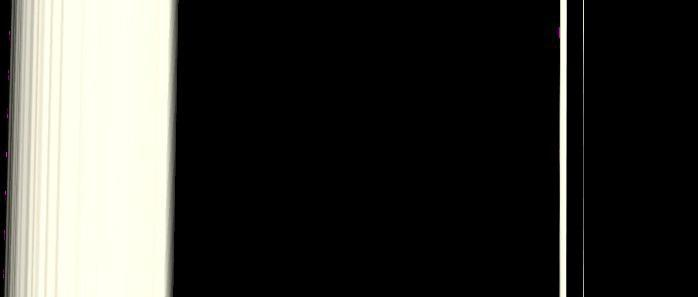
\includegraphics[width=.6\linewidth]{gfx/zoom}
	\caption[Zoom on the side of the shadow]{Zoom on the side of the shadow.}
	\label{fig:zoom}
\end{figure}

\subsubsection*{Infinite Images}

The previous study on the inner halo showed the first step to understand the infinite images of the disk we can see. Let us explain this with more detail: the shadow and the \ac{ISCO} are very close, so near the \ac{ISCO}, the particles turn around the black holes a great number of times. The previous study showed only the case where the particles make one full turn, but between that inner halo and the shadow there are an infinite number of halos.

Why an infinite number of images of the halo? For every turn completed by a geodesic, an image of the halo is generated near the black hole. That is, for every possible turn, a new image is generated.

This explains the infinite number of images, as the number of possible turns is, indeed, infinite. We can zoom even more to see more images of the same disk. 

\autoref{fig:zoom} shows two more halos between the studied halo and the shadow. The left big stripe on the left is what we called before inner halo. We see here that the term is not accurate, as there are more halos between it and the shadow. Greater zooms can be studied in order to see more images of the disk.

This property of the black holes deserves some more attention. A study on the shadow formation and geodesics near the \ac{ISCO} follows.

First of all, let us see \autoref{fig:virtualshadow}. This image depicts parallel geodesics that fall in the black hole. As we can see, the shadow seen on the right part of the image is much greater than the actual diameter of the black hole's horizon. This is due to the greatly curved spacetime, that forces even distant geodesics to curve and fall into the black hole. That way, the shadow is not the black hole's horizon, but the diameter for which the contained geodesics fall inside it.

We can study the \ac{ISCO} by studying geodesics that turn close to the horizon. \autoref{fig:isco} shows two examples of a set of geodesics on the equatorial plane that turn around the horizon once.

\begin{figure}[bth]
	\myfloatalign
	\subfloat[Horizon and shadow]
	{\label{fig:virtualshadow}
		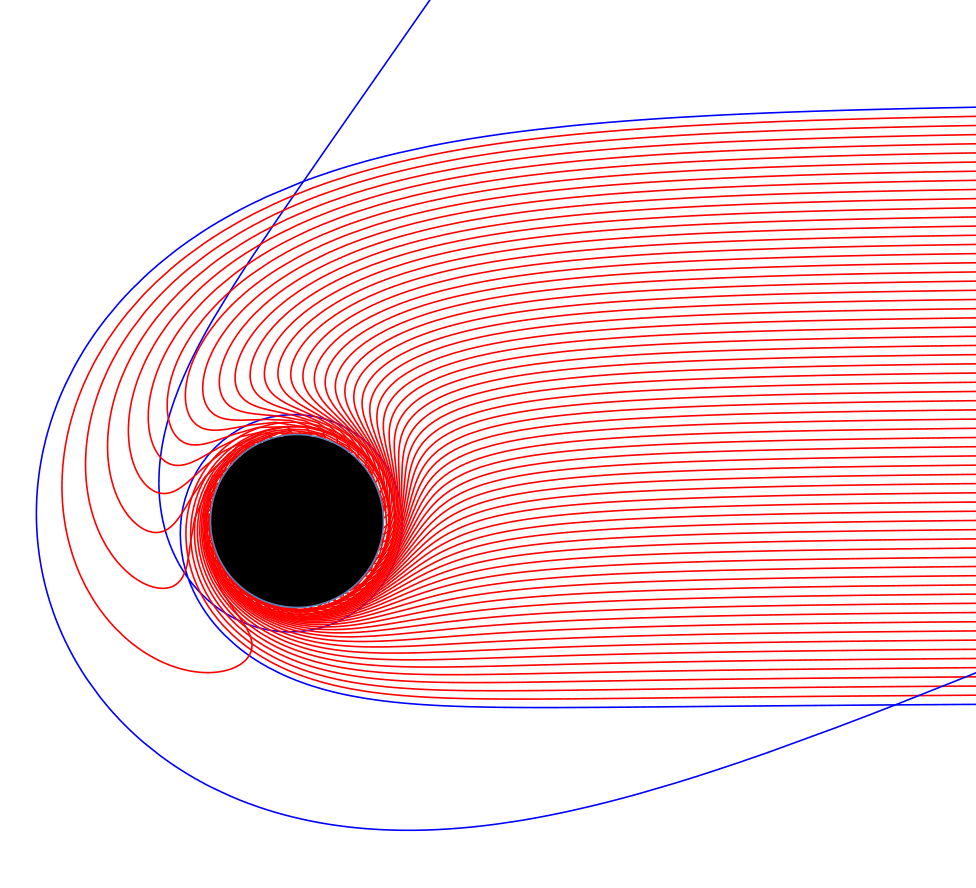
\includegraphics[width=.9\linewidth]{gfx/shadow}} \\
	{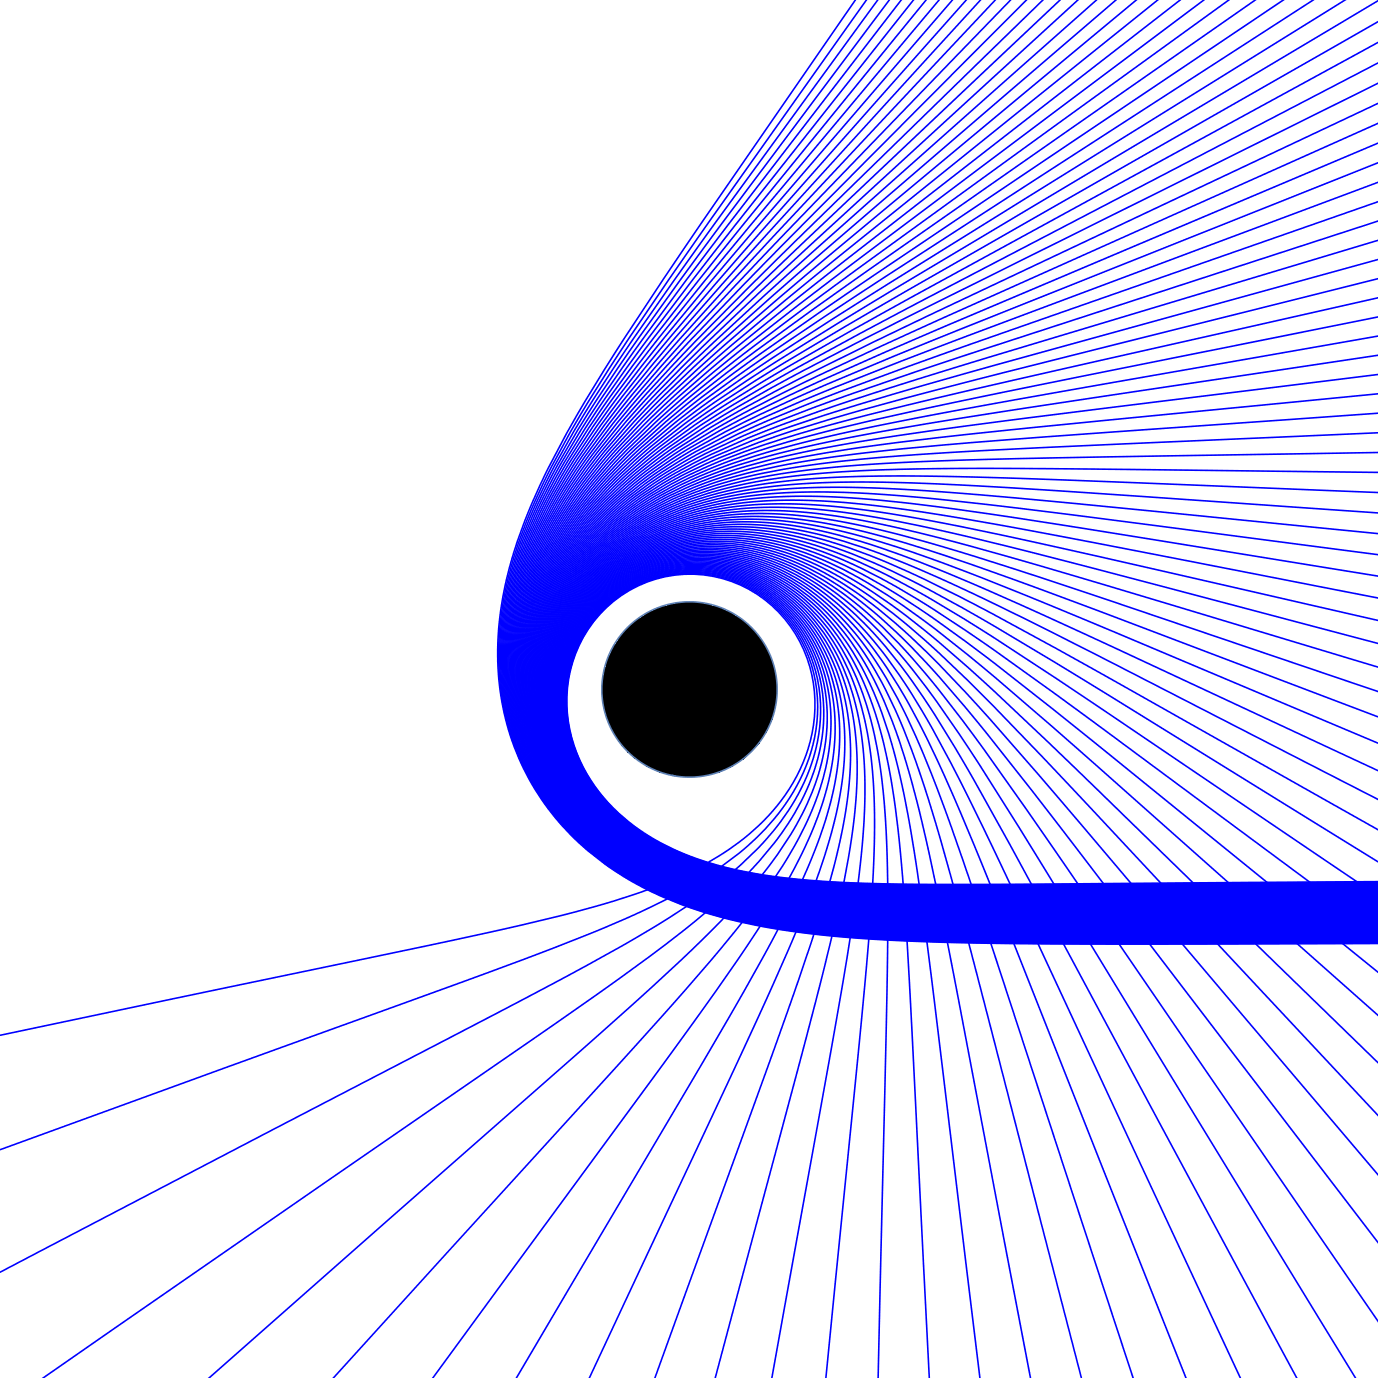
\includegraphics[width=.45\linewidth]{gfx/isco1}} \quad
	{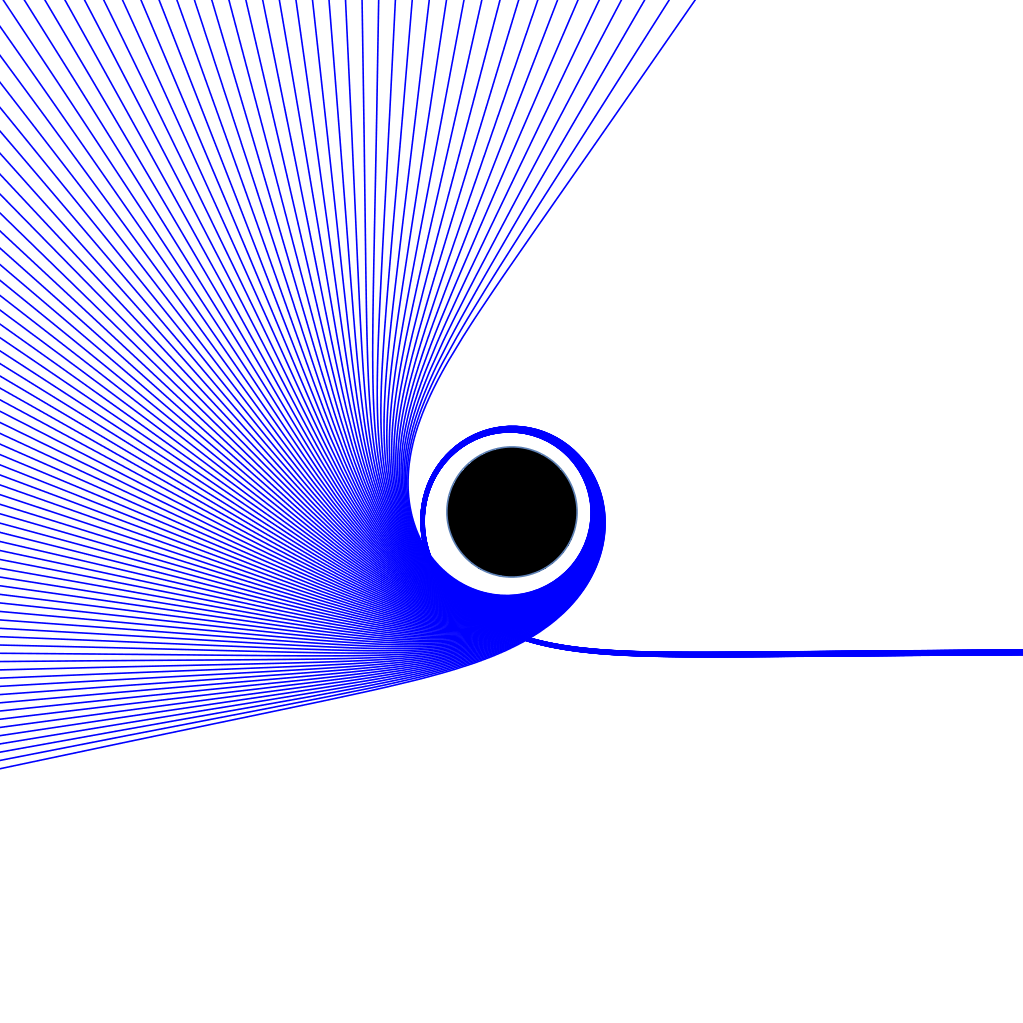
\includegraphics[width=.45\linewidth]{gfx/isco2}}
	\caption[Geodesics around the horizon]{Geodesics around the horizon.}
	\label{fig:isco}
\end{figure}

The number of turns a geodesic can make around the black hole, converging to the \ac{ISCO}, is arbitrary. \autoref{fig:isco4} shows a geodesic that turns up to four times around the black hole's horizon.

In fact, if the geodesic falls into the \ac{ISCO}, the number of turns is infinite, as shown on \autoref{fig:iscofinal}.

All this journey around the black hole explains why the number of images of the disk is infinite: as the geodesic can turn an arbitrary, and therefore infinite, number of times around the black hole, the disk will be infinitely repeated.

\begin{figure}[bth]
	\myfloatalign
	\subfloat[Geodesic turning four times]
	{\label{fig:isco4}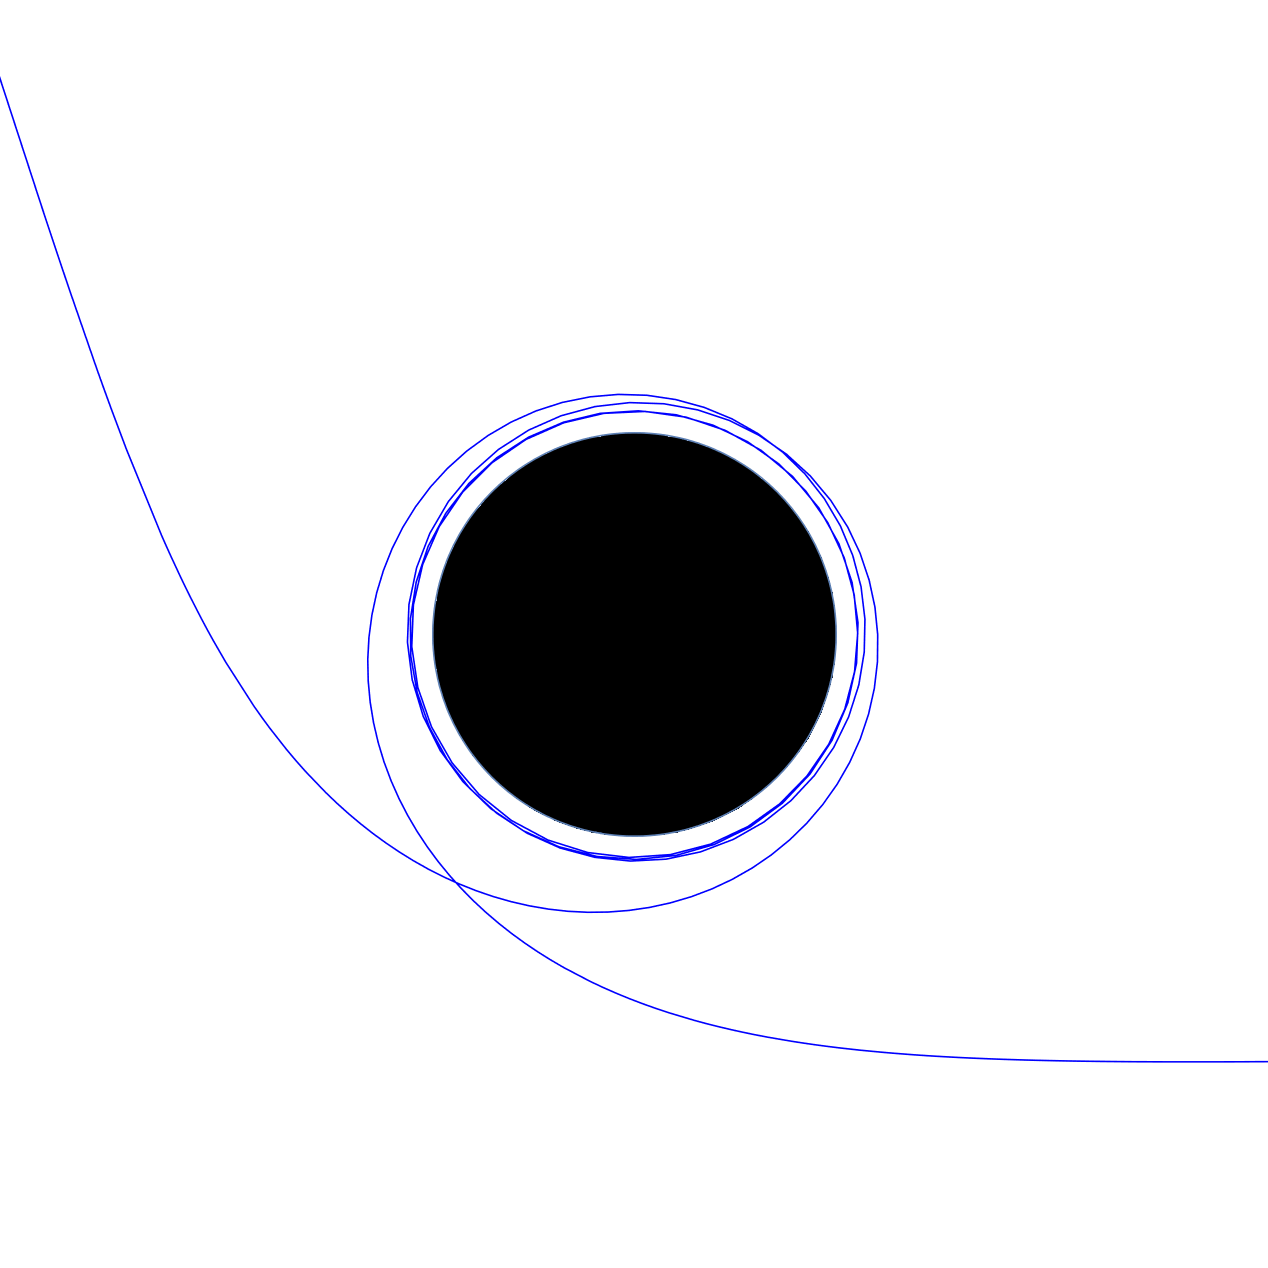
\includegraphics[width=.45\linewidth]{gfx/isco4}} \quad
	\subfloat[Geodesic falling into the ISCO]
	{\label{fig:iscofinal} 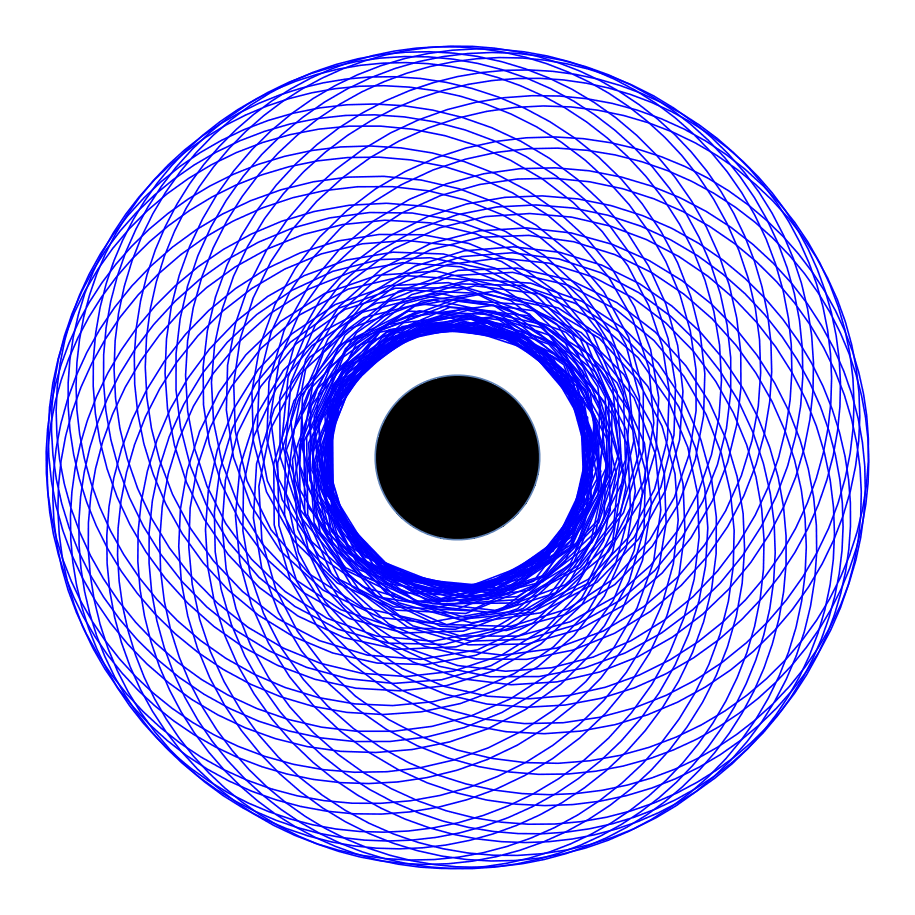
\includegraphics[width=.45\linewidth]{gfx/iscofinal}}
	\caption[Turning geodesics]{Turning geodesics.}
\end{figure}